% !TEX program = xelatex
% !BIB program = bibtex
%
% DEIC — central empirical article (English parallel).
% Compile: xelatex → bibtex → xelatex → xelatex
%
\documentclass[11pt,a4paper]{article}

% === Fonts & Languages ===
\usepackage{fontspec}
\usepackage{polyglossia}
\setmainlanguage{english}
\setotherlanguages{russian,sanskrit,greek}
\setmainfont{DejaVu Serif}[Scale=0.95]
\setsansfont{DejaVu Sans}[Scale=0.95]
\setmonofont{DejaVu Sans Mono}[Scale=0.90]

% === Geometry ===
\usepackage[a4paper,margin=2.5cm,footskip=1cm]{geometry}
\usepackage{setspace}
\setstretch{1.15}

% === Math & Science ===
\usepackage{amsmath}
\usepackage{amssymb}
\usepackage{mathtools}

% === Tables & Graphics ===
\usepackage{graphicx}
\usepackage{booktabs}
\usepackage{tabularx}
\usepackage{longtable}
\usepackage{array}
\usepackage{float}
\usepackage{caption}
\captionsetup{font=small,labelfont=bf}
\usepackage{subcaption}

% === Typography ===
\usepackage{microtype}
\usepackage{csquotes}

% === Cross-refs & Bibliography ===
\usepackage[usenames,dvipsnames,x11names]{xcolor}
\usepackage{hyperref}
\hypersetup{
    colorlinks=true,
    linkcolor=black,
    citecolor=black,
    urlcolor=blue!60!black,
    pdftitle={DEIC: architecture of conditional empathic coupling},
    pdfauthor={I. Bodrov et al.}
}
\usepackage[authoryear,round]{natbib}

% === Section styling ===
\usepackage{titlesec}
\titleformat{\section}{\Large\bfseries}{\thesection}{1em}{}
\titleformat{\subsection}{\large\bfseries}{\thesubsection}{1em}{}
\titleformat{\subsubsection}{\normalsize\bfseries\itshape}{\thesubsubsection}{1em}{}

% === Custom commands ===
\newcommand{\DEIC}{DEIC}
\newcommand{\EAF}{$E_{\mathrm{AF}}$}
\newcommand{\Ecog}{$E_{\mathrm{cog}}$}
\newcommand{\IMM}{\ensuremath{\mathrm{IMM}}}

% === Metadata ===
\title{Architecture of Conditional Empathic Coupling:\\
\large the \DEIC{} measurement framework and a six-factor model of empathy, psychopathy, and attention}
\author{Andrey Bodrov\thanks{Contact: \href{mailto:deic.survey@gmail.com}{deic.survey@gmail.com}.}}
\date{April 19, 2026}

\begin{document}

\maketitle

\begin{abstract}
\noindent
The psychology of empathy has developed for over a century as several poorly integrated lines of research: psychoanalytic theories of defense, attachment theory, cognitive neuroscience, the clinical tradition of psychopathy, and contemplative schools of witnessing. Each glimpsed a fragment of the architecture; none measured the adjacent ones. We introduce \DEIC{} (\textit{Dynamic Empathy and Inner Conflict}), a psychometric measurement framework in which constructs from all of the above traditions acquire a shared coordinate system, making their mutual relations testable within a single sample. In a Russian-language online sample ($N = 1426$), a six-factor oblique CFA validates six distinguishable factors (ID, CA, P, M, $E_{\mathrm{AF}}$, $E_{\mathrm{cog}}$; CFI~=~0.950, RMSEA~=~0.068). A seventh construct --- attention (A), a formative composite reflecting the witnessing function --- enters the conditional process SEM as a moderator. Key findings: \textbf{(1)}~$E_{\mathrm{AF}}$ and $E_{\mathrm{cog}}$ are psychometrically separable; partial $r$(P, $E_{\mathrm{cog}}$) = $+0.32$, supporting the hyper-instrumentation hypothesis in the psychopathic pattern. \textbf{(2)}~Parallel mediation of CA $\to$ \{ID, P, M\} $\to$ $E_{\mathrm{AF}}$ shows the P channel is empty at the population level (CA$\to$P $\approx 0$), making P architecturally orthogonal to childhood history rather than its adaptive consequence. \textbf{(3)}~A narrow conditional process SEM (without P in the $b$ equation) reveals a significant two-stage A-moderation of the CA$\to$ID$\to E_{\mathrm{AF}}$ channel (IMM $= -0.00197$, 95\% CI $[-0.00533, -0.00005]$; $P(\mathrm{IMM} < 0) = 96$--$97\%$ across three Bayesian priors). \textbf{(4)}~In a unified SEM with all paths estimated simultaneously, the $b$-path ID$\to E_{\mathrm{AF}}$ collapses (NS) while P$\to E_{\mathrm{AF}}$ dominates ($-0.726$); this does not overturn the previous findings but restructures them: the ID cascade remains real at case level, but the population-level weight in $E_{\mathrm{AF}}$ is carried by the P-narrative and A as main effect ($+0.393$). \textbf{(5) Trauma is not a verdict.}~The integrated-survivor profile (hi-CA $\times$ hi-A, $n = 118$, 17\%) has the \emph{highest} $E_{\mathrm{AF}}$ in the sample. Childhood history in itself does not fix an adult empathic deficit; it fixes such a deficit only under an intact defensive architecture. Where a witnessing relation to one's own states is present, integrated trauma becomes a resource of empathy rather than its obstacle. \textbf{(6)}~Primary and secondary psychopathy are topologically distinguishable via ID and CA (primary: $n = 144$, ID $\approx 0$, CA $\approx 0$; secondary: $n = 65$, ID $= +0.90$, CA $= +0.98$). \textbf{(7)}~A is valid in the current instrument as a formative composite but not as a reflective latent: A-CFA yields bipolar loadings, and substituting the latent A into the SEM flips the signs of key coefficients --- empirical grounds for treating A as formative and motivating a dedicated A-scale in wave 2. \textbf{(8) Architecture survives multi-modal validation.} The same six-factor structure reproduces across seven methodologically independent channels: latent CFA, network psychometrics (partial $r(\text{P}, E_{\mathrm{cog}}) = +0.32$), free-text behavioral self-identification ($N = 5$ self-described ``pathological liars'' yield $\Delta P = +1.93\,\sigma$), CASE behavioral-anchor choice ($N = 358$ P-signature responders give $\Delta P = +0.92\,\sigma$, $p = 8\times 10^{-46}$), ROC discriminant validity (P AUC $< 0.5$ across all eight diagnostic categories), clinical-visibility asymmetry (only 6 of 1470 use ``formal diagnosis'' even though 489 describe clinical content), and three-path discrimination of somatic-only presentation (Smulevich-blocking, subthreshold-signaling, interoceptive-witness). Such multi-channel coherence is rarely achievable in personality instruments; \DEIC{} is best read not as ``one more empathy questionnaire'' but as an \emph{operational grammar} for distinguishing architecturally opposite configurations producing the same surface presentation. We position \DEIC{} as an \emph{operational dialect} of what the contemplative tradition has distinguished without instruments, directed against the fragmentation of academic psychology --- not as a master-map placed over those schools. The paper formulates falsifiable predictions and states its boundaries (cross-sectional, monolingual, self-report) as part of a planned 18-paper program.

\medskip
\noindent\textit{Keywords:} empathy; psychopathy; dissociation; witnessing; conditional process; psychometrics; contemplative traditions; integrated survivor.
\end{abstract}

\clearpage
\tableofcontents
\clearpage

\section*{How to read this paper}
\addcontentsline{toc}{section}{How to read this paper}
\label{sec:reading_guide}

The paper is long and structured in layers. Different readers come with different interests; below is a short map of which sections carry the most content for each audience, and how one might read the paper non-linearly along a personal route.

\begin{center}
\begin{tabular}{p{0.33\linewidth}p{0.60\linewidth}}
\toprule
\textbf{If you come from\dots} & \textbf{Minimal reading route} \\
\midrule
\textbf{clinical practice} & §\ref{subsec:architecture} (architecture of coupling; primary vs secondary psychopathy), §\ref{subsec:integrated_survivor} (integrated survivor), §\ref{sec:limitations} (what the model does not support), §\ref{sec:falsification} C.1--C.2 \\
\midrule
\textbf{psychometrics} & §\ref{sec:methods}, §\ref{sec:results} 3.1--3.10, §\ref{sec:falsification} Tier A, §\ref{sec:limitations}.3 (statistical limitations) \\
\midrule
\textbf{contemplative or psychodynamic tradition} & §\ref{subsec:A_as_field_condition} (A as field condition), §\ref{subsec:positioning} (positioning against Wilber), §\ref{sec:falsification} D.1 \\
\midrule
\textbf{moral philosophy and law} & §\ref{subsec:architecture} (architecture vs deficit), §\ref{sec:falsification} D.2 (P as an orthogonal moral layer) \\
\midrule
\textbf{methodology and open science} & §\ref{sec:methods}~--~\ref{subsec:analytic_primer} (primer), §\ref{sec:falsification} (falsification commitments), §\ref{sec:limitations} (self-selection, self-report, cross-sectional) \\
\midrule
\textbf{theory and program} & \S\ref{sec:discussion}, §\ref{sec:future}, \texttt{PROGRAM\_STRUCTURE.md} \\
\bottomrule
\end{tabular}
\end{center}

\paragraph{A brief reference for the six factors.} To avoid returning to the definitions each time, below is a one-page summary of what each of the six published factors measures, its reliability in our data, and its conceptual roots.

\begin{center}
\small
\begin{tabular}{p{0.08\linewidth}p{0.22\linewidth}cp{0.23\linewidth}p{0.30\linewidth}}
\toprule
\textbf{Factor} & \textbf{What it measures} & \boldmath$\omega$ & \textbf{Wave-1 parent} & \textbf{Key lines of thought} \\
\midrule
ID & Internal dissonance: affective response is triggered but does not complete; conflict between affective impulse and blocking & 0.91 & IDS (Internal Dissonance Scale) + S, D, AIS, F as surface manifestations & \citet{ferenczi1933, klein1946, fonagy2002}; defenses as a network \citep{digiuseppe2024} \\
\midrule
CA & Childhood alienation: early relational history in which the child's inner states did not meet an adequate response & 0.89 & ACE + CA merged into a single latent & \citet{bowlby1969, main1986, fonagy2002}; early neglect as a predictor of defensive architecture \\
\midrule
P & The moral narrative ``this is permitted to me'': a layer of permission to instrumentally use others, structurally separable from affective architecture & 0.93 & P wave-1 (unchanged) & \citet{cleckley1941, hare1991, blair2013, baroncohen2011}; LSRP \citep{levenson1995} \\
\midrule
M & Masking: a regulatory layer between internal state and external presentation. \textbf{Poorly differentiated} ($r_{\mathrm{lat}}(M, P) = +0.82$); carries no independent claims & 0.55 & MS wave-1 & Impression management; redesign scheduled for wave~2 \\
\midrule
\EAF{} & Affective empathy: automatic resonance with another's state & 0.90 & E (general), post-hoc split & \citet{davis1983, shamaytsoory2011, decety2011} \\
\midrule
\Ecog{} & Cognitive empathy: recognition and understanding of others' mental states without mandatory affective resonance & 0.89 & E (general), post-hoc split & \citet{baroncohen2011, shamaytsoory2011} \\
\bottomrule
\end{tabular}
\end{center}

Plus the seventh construct --- \textbf{attention (A)}, operating as a formative composite (not a reflective latent), instrumented through 31 items drawn from 9 scales with theoretically weighted coefficients. A is not a content of the psyche but a condition of its organization (§\ref{subsec:A_as_field_condition}). A dedicated A-scale is planned for wave~2.

\paragraph{The D--P--A architectural triad.} In the working language of the paper and the broader program we use the short label \textbf{D--P--A} for three content-distinct axes of the architecture. The label is an inheritance from the earliest instrument versions, in which \textbf{D} denoted the general \emph{Defense} bundle --- an aggregate of all defensive subscales (suppression, dissociation, affective isolation, flattening, internal dissonance), not any single one of them. In the current model the functional role of this bundle is carried by the latent \textbf{ID}: the same set of defenses absorbed into a single psychometric construct on the basis of empirically high mutual correlations among subscales ($r = 0.77$--$0.94$) and convergence with network-analytic results on defenses \citep{digiuseppe2024}. We keep the three-letter label because it is content-convenient: it names three functionally and ontologically distinct layers of one system.

\begin{center}
\begin{tabular}{clp{0.62\linewidth}}
\toprule
\textbf{Axis} & \textbf{Latent} & \textbf{Function} \\
\midrule
\textbf{D} & ID & \textbf{Passive} non-coupling. The affective signal is triggered but does not propagate: blocking, suppression, dissociation, affective isolation, affective flattening as surface manifestations of one field. Etiologically --- via CA (childhood alienation). Ego-dystonic: the subject \emph{wants} to feel but cannot. \\
\midrule
\textbf{P} & P & \textbf{Active} non-coupling. Affective resonance is structurally available but fires conditionally; accompanied by the moral narrative ``this is permitted to me''. Etiologically --- orthogonal to CA at the population level. Ego-syntonic: the subject \emph{chooses} not to feel. \\
\midrule
\textbf{A} & A (formative) & \textbf{Condition of the field}, not its content. The witnessing relation, metacognitive awareness. Ontologically asymmetric to D and P: not one more function, but the mode in which other functions exist. In our data --- moderator of both stages of the CA$\to$ID$\to$\EAF{} channel (in the narrow specification) and the main positive predictor of \EAF{} in the unified model. \\
\bottomrule
\end{tabular}
\end{center}

Accordingly, when the text speaks of ``the D-channel'' or ``the D-pattern'' it refers to the passively-blocking architecture anchored psychometrically by the ID latent; ``the P-channel'' refers to the active-narrative architecture; ``the A-layer'' refers to the witnessing meta-level. Type descriptions follow from this: primary psychopathy --- \textbf{P without D}; secondary psychopathy --- \textbf{P with D}; integrated survivor --- \textbf{D with A}; baseline empathic pattern --- \textbf{neither D nor P}.

\paragraph{Methodological glossary.} To avoid translating technical terms inline, the table below records the canonical Russian--English correspondences for the methodological vocabulary used in the paper. Where an English term is preserved in both versions (acronyms, names), this is marked.

\begin{center}
\small
\begin{tabular}{p{0.38\linewidth}p{0.56\linewidth}}
\toprule
\textbf{Russian term in the original} & \textbf{English equivalent / clarification} \\
\midrule
подтверждающий факторный анализ, CFA & confirmatory factor analysis (CFA) \\
эксплоративный факторный анализ & exploratory factor analysis (EFA) \\
косоугольная / ортогональная CFA & oblique / orthogonal CFA \\
латентный фактор, латентная переменная & latent factor / latent variable \\
факторная нагрузка & factor loading \\
факторные оценки & factor scores \\
индексы соответствия & fit indices \\
индекс сравнительного соответствия & Comparative Fit Index (CFI) \\
средняя ошибка аппроксимации & Root Mean Square Error of Approximation (RMSEA) \\
бифакторная модель & bifactor model \\
доля объяснённой общей дисперсии & Explained Common Variance (ECV) \\
иерархическая омега & hierarchical $\omega$ \\
главный эффект / эффект взаимодействия & main effect / interaction effect \\
модерация & moderation \\
медиация & mediation \\
параллельная медиация & parallel mediation \\
непрямой эффект / путь~$a$, путь~$b$, прямой путь $c'$ & indirect effect / $a$-path, $b$-path, direct path $c'$ \\
модерированная медиация & moderated mediation \\
двойно-модерированная медиация & moderated-moderated mediation \\
индекс двойно-модерированной медиации & Index of Moderated-Moderated Mediation (\IMM) \\
объединённое структурное уравнение & unified SEM \\
бутстрэп / бутстрэповский доверительный интервал & bootstrap / bootstrap confidence interval \\
апостериорное распределение, байесовский постериор & Bayesian posterior \\
приор, априорное распределение & prior \\
95\%-ный интервал наивысшей плотности & 95\% highest density interval (HDI) \\
масштабирующий множитель, коррекция Саторра--Бентлера & Satorra--Bentler scaling factor \\
рефлексивный / формативный конструкт & reflective / formative construct \\
контроль переменной, частная корреляция & partialling / partial correlation \\
робастность, проверка устойчивости & robustness check \\
метод расщеплённой половины & split-half method \\
инвариантность измерения & measurement invariance \\
конфигуральная / метрическая / скалярная инвариантность & configural / metric / scalar invariance \\
характеристическая кривая, площадь под кривой & ROC curve / area under the curve (AUC) \\
\bottomrule
\end{tabular}
\end{center}

\paragraph{What this paper does not do.} To prevent misdirected expectations: this is \emph{not} a longitudinal study, \emph{not} a clinically validated scale with cut-off scores, \emph{not} a cross-cultural validation, \emph{not} an attempt to replace DSM. It is the first empirical validation of a six-factor architecture on a Russian-language online sample, with an explicit list of what subsequent waves of the program will have to test (§\ref{sec:falsification}, §\ref{sec:future}). Cross-sectional, self-report, monolingual.

\clearpage

\section*{Glossary: DEIC and Key Terms}
\label{sec:glossary}
\addcontentsline{toc}{section}{Glossary}

This paper was written at the intersection of psychometrics, clinical psychology, and contemplative traditions. To keep readers from getting caught on technical vocabulary, brief definitions are collected here. Each term is introduced in the main text with its English expansion on first use; abbreviated forms are used thereafter in tables and formulas.

\subsection*{Central DEIC constructs}

\begin{description}
    \item[DEIC] \textit{Dynamic Empathy and Inner Conflict} --- the name of the measurement framework and of the 131-item instrument derived from it.
    \item[ID (Internal Dissonance)] \textbf{internal dissonance} --- a state in which an empathic response has already begun but is then blocked because the affective material is intolerable \emph{in itself}, whether someone else's or one's own; these two directions are symmetrical in ID and reflect a single containing function. Experienced as ``I want to feel but I cannot,'' not only toward another but toward oneself. A passive defense, a low ``permission'' for feeling in both directions simultaneously.
    \item[CA (Childhood Alienation)] \textbf{childhood alienation} --- early family-emotional history: absence of responsiveness from significant adults, inability to be oneself, a pervasive sense of unsafety in one's closest circle. Not a sum of traumatic events but a climate.
    \item[P (Psychopathy)] \textbf{psychopathic pattern} --- an architecture in which empathy is \emph{not blocked} but \emph{conditional}: I feel whoever I choose to feel, and I can ``switch'' that channel at will. In DEIC, a morally neutral coordinate, not a diagnosis.
    \item[M (Masking)] \textbf{masking} --- social presentation that diverges from inner state. The current scale is weak ($\omega = 0.55$); it will be redesigned in wave 2.
    \item[E\textsubscript{AF} (Affective Empathy)] \textbf{affective empathy} --- capacity for direct emotional resonance: another's pain registers in one's own body as one's own.
    \item[E\textsubscript{cog} (Cognitive Empathy)] \textbf{cognitive empathy} --- capacity to understand another's inner state as a model, as a mental map, without obligatory bodily resonance. The kind of empathy that can be trained, and that is used by the interrogator, the psychopath, and the skilled therapist --- each in their own way.
    \item[A (Attention / Witnessing)] \textbf{witnessing attention, presence} --- a metacognitive capacity to observe one's own states without merging with them. Closest to what contemplative traditions call satipa\d{t}\d{t}h\=ana (Buddhism), s\=ak\d{s}\=i (Advaita), rigpa (Dzogchen), self-remembering (Gurdjieff). In DEIC, not content but the condition of observation.
\end{description}

\subsection*{Psychometric methods}

\begin{description}
    \item[Latent factor] --- a hypothesized inner characteristic that cannot be measured directly but can be reconstructed from the collective pattern of responses to a set of items. ``Conscientiousness,'' for example, is not a single question but the common element joining answers across a dozen items.
    \item[EFA] \textit{exploratory factor analysis} --- ``how many latent characteristics are needed to account for the structure of the responses?'' Used when theory does not yet fix the number of factors.
    \item[CFA] \textit{confirmatory factor analysis} --- ``do the items group as theory predicts?'' A test, not an exploration.
    \item[SEM] \textit{structural equation modeling} --- a method in which several regressions are estimated simultaneously, with latent variables and paths among them. Permits questions such as ``does predictor A affect outcome C directly, or only through mediator B?''---answered within a single system of equations.
    \item[Reflective latent] --- the classical model: the latent factor \emph{generates} its observed items; changes in factor level are reflected across all items simultaneously. Items are interchangeable indicators.
    \item[Formative composite] --- the opposite construction: a set of heterogeneous items \emph{sum} into a resultant quantity that does not reflect a single underlying property. Removing an item changes the meaning of the composite. A in DEIC is organized in exactly this way.
    \item[Factor score] --- the estimated value of a latent factor for each participant, derived from CFA; used as a variable in subsequent analyses.
    \item[$\omega$ (McDonald's omega)] --- a modern measure of internal consistency (reliability), the preferred alternative to Cronbach's $\alpha$. Values above $0.80$ are acceptable; above $0.90$, high reliability.
    \item[Parcels] --- aggregated mini-composites of 3--5 items each, used in place of raw items in CFA. Reduce the number of model parameters and smooth item-level noise.
    \item[Two-level scoring (DEIC wave 2)] --- a proposed instrument architecture in which each item carries \emph{two} technical fields: \texttt{factor\_weights} (a vector of weights across several factors, used in CFA/SEM, preserving the item's theoretical multidimensional content) and \texttt{primary\_scale} (the single factor into which the item enters under composite sum-scoring). The separation eliminates the algebraic inflation of between-composite correlations characteristic of naive multi-scale scoring, while preserving multi-scale weights as a \emph{theoretical} a priori declaration. Distinct from ``one item = one factor'' in that cross-loadings remain within the model rather than being struck out.
\end{description}

\subsection*{Causal path analysis}

\begin{description}
    \item[Mediation] --- the situation in which A affects C not directly but \emph{through} an intermediate variable B. Example: childhood alienation affects affective empathy not directly but through the formation of internal dissonance.
    \item[a-path] --- the link A $\to$ B (predictor acts on mediator).
    \item[b-path] --- the link B $\to$ C (mediator acts on outcome).
    \item[Direct effect (c$'$)] --- the portion of the influence of A on C that remains after the mediator is taken into account.
    \item[Indirect effect] --- the portion of the influence of A on C that passes through the mediator (the product a $\cdot$ b).
    \item[Moderation] --- the ``under what conditions'' situation: the effect of A on B is not constant but depends on the level of a third variable M. In DEIC, A moderates both the a-path (CA $\to$ ID) and the b-path (ID $\to$ E\textsubscript{AF}).
    \item[Interaction (A $\times$ B)] --- the formal expression of moderation in regression: the product of two variables, whose coefficient indicates the nonlinearity of their joint effect.
    \item[IMM] \textit{index of moderated-moderated mediation} --- the product of two interaction coefficients ($a_{\text{mod}} \times b_{\text{mod}}$). If IMM differs significantly from zero, the moderator acts on the \emph{entire chain} A$\to$B$\to$C simultaneously, not on a single link. In DEIC, a negative IMM means that high witnessing attention breaks the cascade ``trauma $\to$ dissonance $\to$ empathy block'' at both ends at once.
    \item[Bootstrap] --- a procedure of repeated resampling with replacement (typically 2{,}000--5{,}000 replicates) used to estimate confidence intervals for complex coefficients when a closed-form solution is unavailable.
    \item[95\,\% CI (confidence interval)] --- the range within which the true value of the coefficient is located with 95\,\% probability. If the CI excludes zero, the effect is significant at $p < 0.05$.
\end{description}

\subsection*{Model fit indices}

\begin{description}
    \item[$\chi^2$ (chi-square)] --- a statistic of model--data discrepancy. On its own, almost always significant in large samples; therefore evaluated together with the indices below.
    \item[df (degrees of freedom)] --- the number of independent constraints against which the model is tested; higher df implies a more parsimonious model.
    \item[CFI] \textit{comparative fit index} --- $>0.90$ acceptable, $>0.95$ good.
    \item[TLI] \textit{Tucker--Lewis index} --- related to CFI, slightly stricter with respect to model complexity.
    \item[RMSEA] \textit{root mean square error of approximation} --- $<0.06$ good, $<0.08$ acceptable, $>0.10$ poor.
    \item[Satorra--Bentler scaling] --- a correction to the chi-square for nonnormal data; especially important for Likert-type responses.
    \item[MLR] \textit{robust maximum likelihood} --- an estimation method with standard errors robust to nonnormality. A reviewer-level standard for survey data; requires R/lavaan.
\end{description}

\subsection*{Clinical and theoretical terms}

\begin{description}
    \item[ACE] \textit{adverse childhood experiences} --- a scale of adverse childhood experiences; used in DEIC as a covariate and as a component of composites.
    \item[Primary psychopathy (Karpman, 1941)] --- a type with low internal dissonance and no pronounced childhood trauma; ``constitutional'' coldness, minimal emotional reactivity.
    \item[Secondary psychopathy] --- the same psychopathic pattern of switchable empathy, but with high ID and high CA; a ``trauma-born'' path with a fundamentally different therapeutic profile.
    \item[Integrated survivor] --- a profile with high CA (severe childhood) and high A (developed attentional work); in our sample this profile exhibits the \emph{highest} affective empathy. The empirical anchor for the thesis ``trauma is not a verdict.''
    \item[Hyper-instrumentation] --- the hypothesis (Blair, Baron-Cohen) that the psychopathic pattern does not \emph{reduce} but \emph{sharpens} cognitive empathy, using it as an instrument. In DEIC this is supported by the positive partial correlation $r(\text{P}, \text{E}_{\text{cog}}) = +0.32$ after controlling for shared sources of variance.
    \item[Free will (operational)] --- in DEIC, not a binary metaphysical property and not an illusion, but a \emph{graded operational variable}: the magnitude of the gap between the automatic stimulus--response coupling (the working of the D/P/E configuration) and the observation of that coupling (A). Zero A $\Rightarrow$ behavior is functionally determined by the current configuration; high A $\Rightarrow$ the space of choice grows, in proportion to the momentary capacity to hold a witnessing stance. This is an operationalization of what traditions describe as ``awakening,'' ``liberation,'' ``slave of the will,'' ``self-remembering''; not a solution to the metaphysical problem of free will but a refocusing of it into a measurable psychological variable.
\end{description}

\subsection*{Contemplative references}

\begin{description}
    \item[Satipa\d{t}\d{t}h\=ana] (P\=ali Buddhism) --- ``establishment of mindfulness''; the systematic practice of observing body, feelings, states of mind, and phenomena.
    \item[S\=ak\d{s}\=i] (Advaita Ved\=anta) --- ``the witness''; that in experience which remains unchanging as contents shift.
    \item[Rigpa] (Tibetan Dzogchen) --- knowing-presence, nondual awareness prior to the subject--object split.
    \item[Self-remembering] (Gurdjieff, the Fourth Way) --- the practice of holding self-awareness in parallel with engagement in action; the closest Western equivalent of witnessing.
    \item[Anti-Wilber (disciplinary rule)] --- the refusal of a hierarchical ``master map'' overlaid on traditions. DEIC is positioned as an operational dialect of what traditions have already seen, not as a meta-map above them.
\end{description}

\subsection*{Neuroscientific references}

\begin{description}
    \item[DMN] \textit{default mode network} --- active during mind-wandering and self-referential processes. A candidate neural correlate of what A in DEIC measures at the phenomenological level.
    \item[Predictive coding] --- a neuroscientific framework in which the brain operates as a device that continuously predicts its sensory input and corrects its model by prediction errors. Used in this paper as a candidate account of the difference between ID (bottom-up overload) and P (top-down model selection).
\end{description}

\clearpage

\section{Introduction}
\label{sec:introduction}

\subsection{Empathy as a field: a hundred years of scattered contacts}

From the early psychoanalysts \citep{ferenczi1933, klein1946} through contemporary cognitive neuroscience \citep{decety2011, singer2014}, the psychology of empathy has accumulated several major, internally rich, but poorly articulated lines of inquiry. The psychoanalytic tradition describes splitting, repression, and the defensive mechanisms that turn the experience of the other into its opposite \citep{freud1915, fairbairn1952, bion1962, fonagy2002}. Attachment theory develops environmental antecedents---the quality of early relationships as a predictor of adult affective resonance \citep{bowlby1969, main1986, lyonsruth1999}. Cognitive neuroscience separates cognitive empathy (theory of mind) from affective empathy (resonance), pointing to distinct neural substrates \citep{shamaytsoory2011, decety2011}. The mirror-neuron literature proposes a biological mechanism of affective resonance \citep{rizzolatti2004, iacoboni2009}. The clinical tradition of psychopathy, from \citet{cleckley1941} through \citet{hare1991} and \citet{blair2013}, treats affective deficit as a structural property of a specific subpopulation. Contemplative traditions, from the Buddha to contemporary nondual literature \citep{godman1985, dunne2011, josipovic2014}, describe a distinct stratum of consciousness---a witnessing stance, meta-awareness---that, according to these traditions, modulates all other psychological functions.

Each of these lines has developed independently, with its own instruments, its own vocabulary, its own validation standards. This is not a theoretical reproach: detailed work within each paradigm yields knowledge that would be impossible under eclectic merger. But it is an empirical problem: the researcher who wishes to measure empathy in a concrete person and to make warranted claims about that person's resources and vulnerabilities finds themselves with five or six partial maps of one territory, none of which covers the whole.

This paper does not propose a seventh map on top of the six existing ones. It proposes a \emph{measurement framework} in which the constructs already measurable within each tradition receive a shared quantitative coordinate system that permits comparison and cross-reference within a single sample. We call this framework \DEIC{} (\textit{Dynamic Empathy and Inner Conflict}---a working name emphasizing the interaction between empathy and defensive mechanisms). Psychometrically, \DEIC{} is a six-factor model with one additional formative construct (attention, A), evaluated by confirmatory analysis on a sample of $N = 1426$.

\subsection{Empathy as default: an inverted measurement frame}
\label{subsec:empathy_as_default}

Before describing the specific factors of the model, we state the inverting thesis on which \DEIC{} is built and which distinguishes it from most existing empathy instruments. The standard measurement tradition---from IRI \citep[Interpersonal Reactivity Index;][]{davis1983} through the Empathy Quotient \citep{baroncohen2011} to contemporary multidimensional instruments---proceeds from the implicit premise that empathy is an individual ability varying in magnitude: some people have more of it, others less, and the task of the instrument is to quantify that magnitude. We proceed from the opposite premise.

\textbf{Empathy is the default state of the human psyche.} Affective resonance with another's state is not an achievement, not a resource, not a trait that some have developed and others have not; it is a basic function of the primate social brain \citep{rizzolatti2004, iacoboni2009, decety2011}, neurologically supported by mirror-neuron and affective-resonance systems that operate in infants from the first months of life. \emph{Observed between-person differences in empathy are not differences in its quantity, but differences in the mechanisms that suppress it.} The model therefore proposes to measure not empathy as such, but \emph{the forms and strength of non-empathy}---the active and passive processes that block the underlying capacity.

From this inversion follows a distinction that is the central conceptual instrument of \DEIC{}. There are two architecturally different channels of non-empathy.

\textbf{Passive blocking.} The empathic response begins but is blocked by the defensive system, because the experience itself---\emph{regardless of whether it is another's or one's own}---is intolerable to the psyche in its current configuration. One common oversimplification must be set aside immediately: passive blocking is not a block on ``feeling the other'' separate from ``feeling oneself.'' It is one and the same channel. The capacity to bear affective resonance with another's pain and the capacity to bear one's own inner material are structurally a single function, not two separate ones: the reversible sensitivity of a containing system that either holds affect or does not. The psychoanalytic and mentalization traditions record this explicitly: \citet{bion1962}'s $\alpha$-function---the capacity to metabolize emotional experience---operates symmetrically on one's own and received states; \citet{fonagy2002}'s reflective function is by definition bidirectional (the capacity to mentalize others is predicted by the capacity to mentalize oneself, and vice versa); \citet{winnicott1965}'s holding is possible in the mother precisely to the extent that she can bear her own states. The neurobiological line of \citet{schore2001} shows that the substrate of self-regulation and other-attunement is shared: the right-hemisphere networks responsible for regulating one's own arousal are the same networks that enable affective attunement to another. A person in the regime of passive blocking therefore \emph{cannot} feel in both directions simultaneously: they are equally cut off from tears over another's loss and from their own fatigue, equally blind to rising anxiety in a partner and in themselves. Phenomenologically this appears as numbing, dissociation, affective flattening, an inner conflict of ``I ought to feel but I cannot''---and the ``ought'' applies both to response to the other and to contact with one's own content. The psychometric coordinate is the factor ID (Internal Dissonance). Historical descriptions: \citet{ferenczi1933} on ``identification with the aggressor,'' \citet{klein1946} on splitting, \citet{bowlby1969} and \citet{main1986} on disorganized attachment models, and the clinical dissociative literature \citep{putnam1997, vanderkolk2014}.

\textbf{Active switching-off.} The empathic channel is intact and functionally available, but it does not fire automatically; it engages or disengages depending on contextual suitability and a moral narrative about the situation. A person in this regime \emph{can} feel selectively and can \emph{refrain} from feeling when it is convenient. Phenomenologically this is not numbness but control---smooth switchability. The psychometric coordinate is the factor P (psychopathic pattern). Historical descriptions: \citet{cleckley1941}, \citet{karpman1941}, the clinical tradition \citep{hare1991, lilienfeld1990}, and the neuroscientific line of Blair \citep{blair1995, blair2013}.

These two channels are independent. They are \emph{not} ``the same thing in different proportions'' and do not form a single spectrum. A person may have passive blocking in the complete absence of any psychopathic narrative (the typical clinical profile of depression and complex trauma); may have the conditional psychopathic architecture in the absence of ID (the primary pattern of \citet{karpman1941}, empirically reproduced in our sample at $n = 144$); or may have both at once (the secondary pattern, $n = 65$, $\mathrm{ID} \approx +0.90$ and $\mathrm{CA} \approx +0.98$). Their independence is one of the principal empirical results of this paper (§\ref{subsec:architecture}), and from it follow substantially different clinical strategies.

This inversion of frame is supported by two external empirical anchors that we take to be the strongest arguments in its favor. First, the meta-analytic estimate of \citet{depow2025}: trait measures of empathy explain only 3--15\,\% of the variance in empathic experience in everyday life. If empathy were a stable individual trait that some have and others do not, standard trait instruments would capture a substantially larger share of the variance. The observed 3--15\,\% suggests that the empathic response is a state strongly dependent on situational factors, among which the \emph{activation or deactivation of blocking mechanisms} plays the central role, rather than fluctuations in a baseline resource. Second, the result of \citet{ogawa1997}: absence of parental responsiveness in infancy predicts dissociative symptoms nineteen years later with an effect size of roughly 50\,\% of explained variance---stronger than the prediction from traumatic events themselves. This is consistent with \citet{fonagy2002}'s hypothesis: not the stressful event as such, but the absence of a mentalizing field within which the event could be metabolized, forms the structural dissociative defense. That is, the blocking mechanism forms precisely where the adult capacity to co-experience a child's inner states fails or never arises.

A third anchor is structural. \citet{digiuseppe2024}, in a network analysis of defensive mechanisms, showed that sixteen different defenses form a densely connected integrated system (not independent traits), in which self-assertion serves as the central node and the remaining defenses as peripheral nodes carrying different functional loads. In our data, correlations among subscales of passive blocking (dissociation, suppression, affective isolation, flattening, internal dissonance, masking) lie in the range $r = 0.77$--$0.94$. This is not an instrument-level redundancy artifact but an independent reproduction of what Di Giuseppe's network analysis found on its own: defensive mechanisms are \emph{one integrated functional system}, not a set of parallel individual traits. This is why in our 6-factor CFA these subscales collapse into a single latent factor ID---they are not psychometrically discriminable not because the instrument fails to distinguish them, but because in reality they are different phenomenological expressions of one suppression system.

These three anchors---the low explanatory power of trait empathy, the strong prediction of dissociation through the absence of a mentalizing response, and the network integration of defenses---converge independently on a single conclusion: the central object of measurement is \emph{the mechanisms of non-empathy}, not empathy as a trait. The \DEIC{} model is built on this inversion, and all its subsequent claims should be read through that frame.

\subsection{Five points where traditions have touched without meeting}

The reason the \DEIC{} architecture has a chance of being useful lies not in its ambition but in its narrowness. We have selected for modeling those constructs in which different traditions empirically describe \emph{very similar} phenomena but have lacked a shared instrument to confirm it.

\paragraph{Internal dissonance (ID).}
In the psychoanalytic tradition---splitting and ego splitting-off \citep{ferenczi1933, klein1946}; in attachment theory---disorganized internal working models \citep{main1986}; in the clinical dissociative literature---fragmentation in response to trauma \citep{putnam1997, vanderkolk2014}. All three describe the same phenomenon: a person's inner states bear the mark of active blocking, regulation, defensive work, rather than merely content. Psychometrically this should be a single factor if the instrument is correctly constructed. We show that it is.

\paragraph{Childhood alienation (CA).}
In attachment theory---the absence of a secure base \citep{bowlby1969, ainsworth1978}; in mentalization theory---the absence of a mentalizing response \citep{fonagy2002}; in the clinical ACE literature---stressful childhood events \citep{felitti1998}. CA is the environmental condition in which a child's inner states do not meet an adequate response. We instrument it narrowly (not the full ACE index) because, per Fonagy's hypotheses, it is the \emph{absence of a mentalizing field}, not the occurrence of stressful events as such, that predicts downstream dysregulation. The substantive meaning of this narrow formulation: a child learns to distinguish and hold their own states through an adult capable of seeing and naming those states. If no such adult is available, the child does not lose ``information about others'' separately from ``information about the self''; the child fails to develop the general capacity to metabolize affective experience as such. This is why CA $\to$ ID in our model is not ``trauma reduced empathy toward others''; it is ``the absence of a mentalizing mirror did not permit the capacity to bear affective material in both directions at once to form.'' The clinical signature of an adult with high CA and high ID is uniform impermeability both outward and inward: such a person has access neither to their own sadness nor to a partner's sadness, because the only available mechanism is an automatic joint block, not a selective closure of one direction.

\paragraph{Psychopathy as a moral signature (P).}
The clinical tradition \citep{cleckley1941, hare1991} describes psychopathy in the frame of affective deficit and the instrumental use of others; Blair's neuroscience \citep{blair1995, blair2013}---through reduced amygdalar response to another's distress; evolutionary psychology \citep{mealey1995, lalumiere2001}---as a low-frequency stable strategy. We deliberately do not reproduce the deficit frame. In \DEIC{}, the psychopathic pattern is decomposed into two layers: the \textbf{architectural} (conditional rather than unconditional affective coupling---a morally neutral variation, functional in several social roles; see §\ref{sec:discussion}.5) and the \textbf{narrative} (P---a stable assertion ``this is allowed for me,'' determining how the architecture is used socially). The factor P models the second layer. This two-layer shift---from ``broken function'' to ``architecture plus narrative''---alters the clinical, legal, and political implications and is one of the key contributions of the work.

\paragraph{Cognitive vs. affective empathy (\Ecog{} vs. \EAF{}).}
In neuropsychology---two systems with distinguishable substrates \citep{shamaytsoory2011, decety2011}; in mentalization theory---mentalization vs. embodied empathy \citep{fonagy2002}; in clinical work---the key distinction for understanding why an ``intelligent psychopath'' can be accurate in predicting behavior yet indifferent to suffering. We show empirically that these two constructs are separable and differently related to P. An everyday illustration of this distinction is one of the most structurally informative observations usually ignored in trait-measurement literature: the same person may weep over the fate of a literary or film character and remain cold to the suffering of a concrete real person next to them. This is not a contradiction and not ``hypocrisy''---it is a direct signature of channel splitting. Identification with a narrative (a fictional character within a safe storytelling frame) engages primarily the \Ecog{} line: mentalization of a point of view without automatic affective coupling to a real, threatening, unsafe presence of an other. A real suffering person calls for \EAF{} in its full form---affective resonance in a situation that is not governed by a narrative frame and that can make demands. When \EAF{} is blocked by the defensive structure (ID) or regulated conditionally (P), the \Ecog{} channel remains partially or fully intact, and the person experiences a state in which fictional suffering moves them but real suffering does not. In the DEIC architecture this is not an anomaly but a predictable consequence of the separability of the two channels.

\paragraph{Attention as witnessing (A).}
In the contemplative tradition---\textit{satipa\d{t}\d{t}h\=ana} (Buddhism), \textit{s\=ak\d{s}\=i} (Advaita Ved\=anta), \textit{rigpa} (Dzogchen), ``self-remembering'' \citep[Gurdjieff through][]{ouspensky1949}; in the psychoanalytic tradition---the observing ego \citep{sterba1934, kris1956}; in contemporary mindfulness science---meta-awareness \citep{dunne2011, josipovic2014}; in mentalization theory---the reflective function \citep{fonagy1997}. Each of these lines describes a structurally distinct stratum of consciousness: not the content of the psyche but a \emph{relation of observation} to that content. We return to A repeatedly---it is the most theoretically rich and simultaneously the most difficult to instrument of the factors in the model.

\medskip
An important qualification: we do not claim that \DEIC{} describes these traditions \emph{in full} or that it is the \emph{first} to catch the structure they describe. Each of the literatures listed above has measured its construct at greater depth than we do. Our contribution lies in having measured \emph{all of the listed constructs in one sample, with one instrument, under shared methodological standards}. This makes it possible, for the first time, to test their mutual relations not at the level of theoretical reconstruction but at the level of path-model coefficients.

\subsection{Balkanization as failure mode, not as discipline}

Before turning to method, we state the position openly. The tradition of holding that ``a narrow frame = strict science,'' applied in twentieth-century psychology, has resulted in a situation where incompatible microtheories coexist as the norm and are called a discipline. The theory of narcissism is not coordinated with the theory of psychopathy; neither is coordinated with attachment theory; cognitive empathy is measured with instruments architecturally incompatible with affective empathy. This is precisely what \citet{meehl1978} diagnosed half a century ago as the failure mode of psychological theorizing. Physics, chemistry, and biology demand coherence across scales; psychology has allowed itself to abandon that demand under the rhetoric of ``caution.''

We do not adopt that caution as a virtue. We hold that: if the data contain constructs described by different traditions as the same phenomenon under different names, psychometrics should demonstrate so. If the \DEIC{} architecture makes predictions, it is obliged to state them in falsifiable form---in that manner, not through a ``narrow restriction of scope'' that exempts from testing what the model actually predicts. This is the methodological wager of the paper: ambition in content, discipline in how the question is posed.

\subsection{Positioning: three strata, one sentence}

Relative to three reference planes the work stands as follows. In relation to the \textbf{contemplative tradition} (Buddhism, Advaita, Dzogchen, Hesychasm, Gurdjieff, psychoanalysis at its contemplative edge), \DEIC{} stands in the position of \emph{student-translator}: the constructs these traditions distinguished without psychometric instruments for millennia receive coordinates in our framework---and our contribution lies precisely there, not in a ``new integration.'' In relation to \textbf{academic psychology}, \DEIC{} stands in a \emph{confrontational} position: balkanization is not a discipline but a pathology of the field, and a framework of shared referents for what different schools describe in incompatible languages is something the field should have but does not. In relation to the \textbf{integral tradition} (Wilber and AQAL, structural precedents), \DEIC{} stands in a \emph{structurally inverse} position: not a master map onto which traditions land as special cases, but an operational dialect of those same traditions, deployed against fragmentation.

One sentence: \DEIC{} is an operational dialect of what the contemplative tradition measured without instruments, deployed against the balkanization of academic psychology. Student to the tradition, challenger to the field.

\subsection{What \DEIC{} does not claim}

Because the program is positioned as a framework crossing several traditions, we delimit its scope at the outset. \DEIC{} does \textbf{not} claim:
\begin{itemize}
    \item To be the first or the only unifying framework for empathy. Unification is not our verb.
    \item To contain a final operationalization of A, witnessing, or mindfulness. A in its current form is a formative composite, not a reflective latent; this limitation is empirically established (§\ref{sec:results}.7) and is to be corrected in the following wave.
    \item To replace any of the traditions we cite. Psychoanalysis, attachment theory, the cognitive neuroscience of empathy, the mirror-neuron literature, the clinical tradition of psychopathy, and the contemplative schools each possess depth and specificity within their own paradigms that we do not reproduce.
    \item To offer a theory of consciousness or an explanation of the hard problem \citep{chalmers1995}. We measure \emph{functions} within consciousness; we assert nothing about the nature of subjective experience as such.
    \item To deliver clinical recommendations on the basis of a single sample. Everything clinically prescriptive in the Discussion is formulated as \emph{hypotheses for testing}, not as immediate protocols.
\end{itemize}

These limits are not a reluctant retreat but a structural condition for producing work that does not collapse into a meta-theoretical claim. The program is built out of many narrow, falsifiable studies; this paper is one of them.

\subsection{Structure of the paper}

Section~\ref{sec:methods} describes the DEIC-Inventory, the operationalization of the six factors through a 6-factor oblique CFA, the construction of A as a formative composite, and the statistical approach (conditional process SEM, parallel mediation, unified SEM, A-CFA). Section~\ref{sec:results} presents the factor structure, partial correlations, the central conditional-process analysis, parallel mediation, a unified SEM carrying all paths simultaneously, the empirical confirmation of the integrated survivor, the topological distinction between primary and secondary psychopathy, and the empirical demonstration of the formative nature of A. Section~\ref{sec:discussion} takes up the implications of the architecture, isolates A as an ontologically asymmetric factor (field-condition, not field-content), formulates falsifiable predictions and points of divergence with existing theories, and situates the paper within a future program. Limitations and directions for future work appear in Sections~\ref{sec:limitations} and~\ref{sec:future}.

\section{Methods}
\label{sec:methods}

\subsection{Participants}

Data were collected online through the Russian-language DEIC-Inventory. The total sample is $N = 1426$ after removal of invalid responses (less than 80\% completeness, duplicate identifiers, implausible response patterns). Recruitment was via self-selected volunteers through Telegram channels, VK communities, and the researcher's personal networks. Inclusion criteria: age $\geq 18$, Russian as the survey language (non-native speakers were not excluded, but not specifically targeted). No exclusion criteria were imposed.

Participation was anonymous, without identifiers, without compensation. Voluntary informed consent was obtained on the first screen of the questionnaire. Ethics approval: \textit{[to fill]}.

Sample limitations (addressed in §\ref{sec:limitations}): self-selection bias toward a psychologically curious, reflective audience; language specificity; age skew toward 18--37; absence of clinical diagnostic assessments (all diagnoses are self-reported).

\subsection{Instrument}

The DEIC-Inventory is a 131-question self-report instrument, developed iteratively through several waves of qualitative pilot work and quantitative revision. Items are distributed across 14 scale labels: empathy (E), psychopathy (P), suppression (S), dissociation (D), affective isolation (AIS), flattening (F), internal dissonance scale (IDS), masking (M), adverse childhood experience (ACE), childhood alienation (CA), emotional climate (EC), affective-dissociative indicator (ADI), attention (A), and a lie-scale control (Lie).

Response scale: 5-point Likert (1 = ``strongly disagree'' $\to$ 5 = ``strongly agree''). Some items are reverse-coded as a control for response bias.

Innovative instrument features: separation of \emph{declarative} and \emph{behavioral} wordings in paired items (example: ``I believe empathy is important'' --- declarative; ``I often cancel meetings to be with a friend in distress'' --- behavioral); control of structural artifacts via balanced response-scale direction and reverse-coding; a Lie-scale used as a control covariate in partial correlation analyses. The full item-level specification and weights are available in \texttt{questions.json}.

\paragraph{Technical caveat on the Lie covariate.} In wave 1 the Lie scale is operationalized by a single item (LIE\_1: ``I sometimes tell untruths'') with reverse-coding. A single-item operationalization does not permit internal-consistency estimation and constitutes a methodological limitation acknowledged in §\ref{sec:limitations}; Lie is used face-validly as an indicator of self-presentation pressure, without an $\omega$ estimate. Wave 2 expands Lie to $\geq 6$ items with reported reliability (§\ref{subsec:wave2_design}).

\paragraph{Attention check and QC pipeline.} One attention-check item (CONTROL\_1, instructing respondents to select ``Somewhat agree'') is embedded in the instrument. Respondents who fail the attention check are flagged and excluded from latent analyses; the final $N = 1426$ was obtained from a raw $N = 1470$ after QC filtering (attention check, completion $\geq 80\%$, implausible response patterns, fingerprint-based deduplication, and $e2eTestRunId$ filtering).

\paragraph{Three parallel scoring layers.} The exported dataset contains \texttt{raw\_*} (raw sums prior to standardization), \texttt{score\_*} (theoretically weighted composites with multi-factor weights from \texttt{questions.json}), and \texttt{mapped\_*} (0--100 normalized scale for clinical display). All analyses in this paper use the \texttt{score\_*} layer; \texttt{raw\_*} and \texttt{mapped\_*} are preserved for replication convenience and as inputs for external tooling, respectively.

\paragraph{Product-layer labels not used in formal analysis.} The instrument, within its product infrastructure, additionally assigns each respondent (a) an archetypal label from 12 categories (Trickster, Wanderer, Analyst, \dots{}) and (b) a rule-based composite profile tag (\texttt{psychometrics.json.profiles}: e.g., empathicParadox, defensive\_hardness, modestlyBlocked). Neither layer enters the latent analyses of this paper; they are retained in the exported dataset (\texttt{cluster}, \texttt{profiles}, \texttt{ratio} columns) for use in a separate applied publication. An auxiliary field \texttt{score\_maskarading}, a legacy duplicate of \texttt{mapped\_masking}, persists in the wave-1 export and is scheduled for removal in wave 2.

\paragraph{Item-count heterogeneity note.} Seven records show atypical response counts (121, 124, 127, 130 rather than the canonical 122). These are \emph{valid} responses from early pilot versions of the instrument, collected before the item set stabilized in the final 122-active-item configuration. These respondents are \emph{retained} in the analytic sample alongside the others; at the item level, items absent in their version are handled through standard missing-data procedures (listwise for raw composites with a full-coverage criterion, FIML-equivalent for CFA models).

\subsection{Operationalization of the six factors}
\label{subsec:six_factor_ops}

The present paper works with six content factors drawn from the fourteen scales of the instrument. Below is how each one is constructed for analysis.

\subsubsection{Factors via 6-factor oblique CFA}

The primary operationalization is through latent factors from an exploratory-confirmatory sequence:
\begin{enumerate}
    \item EFA with parallel analysis on split-half A ($N = 713$) identified $k = 6$ as the optimal number of factors.
    \item 6-factor oblique CFA (maximum likelihood, correlated factors) on split-half B ($N = 713$): $\chi^2(120) = 516.04$, $p < .001$, CFI~=~0.950, TLI~=~0.936, RMSEA~=~0.068 (robust bootstrap approximation), $\chi^2/df = 4.30$.
    \item Latent factor scores were extracted via the empirical Bayes regression method.
\end{enumerate}

Factors: \textbf{ID} (Internal Dissonance), \textbf{CA} (Childhood Alienation), \textbf{P} (Psychopathy), \textbf{M} (Masking), \textbf{\EAF{}} (Affective Empathy), \textbf{\Ecog{}} (Cognitive Empathy).

Reliability (McDonald's $\omega$ on latent factor scores): ID~=~0.91, CA~=~0.89, P~=~0.93, \EAF{}~=~0.90, \Ecog{}~=~0.89, \textbf{M~=~0.546}. M reliability is emphatically low; no M-specific claims are made in the paper. M is retained in the model as a coordinate for future revision.

\subsubsection{Attention (A): a formative composite}

A is not one of the six factors drawn from the 14-scale instrument. A is constructed as a formative composite on a theoretical schema: 31 items from 9 scales (E, IDS, D, ADI, AIS, S, EC, CA, P) with a-priori coefficients ranging from $+0.4$ to $-0.4$, reflecting each item's theoretical position relative to the witnessing function. The composite:
\[
A_i = \sum_{j=1}^{31} w_j \cdot x_{ij}
\]
where $w_j$ is the item's theoretical coefficient, $x_{ij}$ is the $z$-standardized response of participant $i$ to item $j$. Items with negative coefficients invert their contribution, so that a high A score denotes elevated witnessing presence.

The coefficients were set through iterative revision with the author's participation; details in \texttt{validate\_attention.py}. In §\ref{sec:results}.7 we empirically check that this formative composite cannot be reduced to a single reflective latent factor.

\subsubsection{Alternative constructions (controls)}

In parallel with the latent factors we used weighted composites (classical implementation via unit weights on primary\_scale). These composites are inflated relative to the latent ones (mean inflation $\sim 0.18$, maximum $0.68$ with sign reversal for P$\leftrightarrow$E); they are reported for comparison, but all content-level conclusions of the paper rest on latent factor scores.

\subsection{Analytic strategy: a reading for non-psychometricians}
\label{subsec:analytic_primer}

This section is written for readers who come to the paper from clinical practice, theory, philosophy, or the contemplative traditions, and who are not expected to read structural-equation jargon fluently. A psychometrically trained reader can jump directly to §\ref{subsec:stat_approach}. Here --- a short, content-accurate explanation of what each of the analyses the paper leans on actually does, and what cannot be read off them.

\subsubsection{Latent factors: why not just sum responses}

If we want to measure empathy, one can take ten empathy questions, sum the responses, and call the sum empathy. That is a \emph{composite score}; it is useful, but it rests on a structural assumption: that all ten questions capture the same thing in the same proportion, and that the measurement noise in them is independent. In practice, part of the variance of responses is the common construct (\emph{what all ten questions actually capture in common}), and part is specific to a given wording, situation, or response style of the respondent. Latent factor analysis separates these two parts explicitly. A factor is an \emph{unobservable} variable reconstructed from the pattern of correlations among items: the assumption is that if empathy exists, then responses to empathy questions should correlate among themselves more than with responses to, say, psychopathy questions. The strength of association between an item and the factor is called a \emph{factor loading}; operationally, ``how much of this item is about empathy, and how much about something else''. When we later speak of \emph{factor scores}, we mean the estimated position of each respondent on the unobservable axis, computed as a weighted combination of their responses, with weights reflecting the loadings. Unlike composites, factor scores automatically \emph{penalize} noisy items and do not inflate cross-construct correlations via shared variance (see §\ref{sec:limitations} on the scoring artifact of multi-scale weights in composite sums).

\subsubsection{Confirmatory factor analysis; oblique vs.\ orthogonal specifications}

In confirmatory factor analysis (CFA) we \emph{pre-specify} which items load on which factor and test whether that structure holds in the data. In contrast to exploratory factor analysis (EFA), where factors are found ``bottom-up'' from the correlation matrix, CFA works ``top-down'': we have a theory, we have data, and we test their compatibility. The result is a set of \emph{fit indices}, described below.

\emph{Oblique vs.\ orthogonal} is the decision whether to allow factors to correlate. Orthogonal CFA fixes all inter-factor correlations at zero --- mathematically convenient, but almost always wrong in psychology: empathy and psychopathy \emph{do} correlate negatively, ID and CA \emph{do} correlate positively, and forcing these correlations to zero means distorting the data for model simplicity. The oblique CFA we use allows factors to correlate and estimates those correlations directly. This is substantive: inter-factor correlations are part of the result, not a nuisance.

\subsubsection{Fit indices: what they say and what they do not}

When we write ``CFI = 0.950, RMSEA = 0.068, $\chi^2/df = 4.30$'', each number carries a specific intuition.

\textbf{$\chi^2$ statistic} measures how far the observed covariance matrix of items diverges from that predicted by the model. If the model is perfect, the divergence is zero; the larger the divergence, the larger $\chi^2$. The catch: $\chi^2$ grows with sample size; at $N = 1426$ even a very good model is typically rejected by a strict $\chi^2$ test. Hence in modern psychometrics $\chi^2$ is read as description rather than test, and is complemented by relative indices.

\textbf{CFI (Comparative Fit Index)} compares the model to a ``null'' model in which all items are independent (no factor structure at all). CFI = 0.950 means that our model closes 95\% of the distance between the null model and a perfect one. Conventional cutoffs: $\geq 0.95$ good, $\geq 0.90$ acceptable. CFI is much less sensitive to $N$ than $\chi^2$.

\textbf{RMSEA (Root Mean Square Error of Approximation)} is the mean model error per degree of freedom. Intuitively, ``by how much does the model miss the data on average per parameter''. Conventional cutoffs: $\leq 0.05$ good, $\leq 0.08$ acceptable. RMSEA = 0.068 is acceptable for a complex model on real data.

\textbf{$\chi^2/df$} is the ratio of $\chi^2$ to degrees of freedom; a crude check on ``is the misfit bigger than what chance would produce''. $\leq 5$ is acceptable for large samples.

Important caveat, repeated throughout the paper: these indices assume multivariate normality, which our data violate (Mardia $p < 0.0001$). We therefore report both standard maximum-likelihood (ML) indices and robust Satorra--Bentler--corrected ones, and anchor all substantive conclusions on latent factor scores, which are less sensitive to that correction.

\subsubsection{Bifactor models: one general factor plus specific residuals}

In §\ref{subsec:id_bifactor} we apply a \emph{bifactor} model to the five wave-1 scales of passive blocking: \textbf{SUP} (Suppression), \textbf{DIS} (Dissociation), \textbf{AIS} (Affective Isolation Scale), \textbf{FLA} (Flattening), and \textbf{IDS} (Internal Dissonance Scale --- the historical ``parent'' name from which the final latent takes its label, ID). This is a special CFA architecture in which one general factor (ID\textsubscript{g}) loads on \emph{all} items, and, in addition, \emph{orthogonal} specific factors (one per subscale) load only on their ``own'' items. This allows variance to be decomposed algebraically: how much is absorbed by the general construct, and how much remains in subscale-specific residuals. The \textbf{ECV (Explained Common Variance)} metric $= 0.571$ states that 57\% of common factor variance is explained by the general ID; the remaining 43\% sits in specifics. Per-subscale ECV is the same metric computed within one subscale: for SUP (Suppression) it is 0.31, meaning that suppression is to a large extent \emph{not} about general ID but about something of its own. The value of this analysis for wave~2 is a structural basis for item redesign.

\subsubsection{Mediation, moderation, parallel mediation}

\emph{Mediation} answers the question ``through what''. If CA predicts \EAF{} but we hypothesize that the prediction runs not directly but through ID, we test mediation. Formally: path $a$ (CA $\to$ ID), path $b$ (ID $\to$ \EAF{} controlling for CA), direct path $c'$ (CA $\to$ \EAF{} controlling for ID). The indirect effect is $a \cdot b$; the total effect is $a \cdot b + c'$. Statistical significance of the indirect effect is tested via the 95\% bootstrap confidence interval: if the interval excludes zero, mediation is significant.

\emph{Moderation} answers a different question --- ``under what conditions''. A moderator is a variable that changes the \emph{strength} of the association between two other variables. In regression it is an interaction term: ID $\times$ A in the \EAF{} equation. If the interaction coefficient is significant, the strength of ID $\to$ \EAF{} varies with the level of A.

\emph{Parallel mediation} is the extension: one predictor (CA), one outcome (\EAF{}), several mediators (ID, P, M) estimated \emph{simultaneously}. Each obtains its own indirect effect (through itself), and we can test which of them are significant and which are empty. In our case the CA$\to$P$\to$\EAF{} channel turned out empty: it exists formally but carries no variance. Substantively: P is architecturally orthogonal to childhood history.

\subsubsection{Moderated-moderated mediation and the \IMM{} index}

Moderated-moderated mediation is the case in which \emph{both} stages of the mediation channel ($a$ and $b$) are moderated by the same variable. In our central specification, A moderates both CA$\to$ID (the first stage) and ID$\to$\EAF{} (the second stage). Question: do these moderations combine into a coherent picture, or are they independent?

The \textbf{Index of Moderated-Moderated Mediation (\IMM)} \citep{hayes2018} is the product of the two interaction coefficients: $a_{\text{mod}} \times b_{\text{mod}}$. Intuitively, ``by how much does the indirect effect change when the moderator shifts by one unit on both stages at once''. If \IMM{} is significant, the channel as a whole is reorganized by the moderator rather than merely receiving additional noise. Tested via a bootstrap confidence interval.

Key intuition for the reader used to simple interactions: ordinary moderation answers ``does the strength of an association depend on a condition?''; \IMM{} answers ``does the \emph{whole chain} depend on the condition in a single, coherent way?''. This is stronger than simple moderation and weaker than a claim of fully reorganized architecture. Fig.~\ref{fig:imm_intuition} shows this graphically.

\subsubsection{Reflective vs.\ formative constructs}

This distinction carries the entire discussion of A (§\ref{subsec:A_as_field_condition}, §\ref{sec:limitations}). In the classical psychometric model a construct is \emph{reflective}: it is the cause of its indicators. Empathy ``produces'' high answers on empathy items; if you really have empathy, it manifests across several connected behaviors. Three consequences follow: indicators should correlate positively among themselves, should have positive loadings on the general factor, and removing one indicator does not change the meaning of the construct.

A \emph{formative} construct is the reverse: indicators are not consequences but \emph{constituent parts}. A classical example is socioeconomic status: income, education, and occupation are not symptoms of SES, but components from which SES is assembled. Removing income from an SES model changes the construct itself. Indicators of a formative construct need not correlate positively, and loadings can be \emph{bipolar}: if one component is positive and another negative, this is not a contradiction but a structural feature.

In §\ref{sec:results} and §\ref{sec:limitations} we show that A in the present item pool behaves as a formative composite, not a reflective latent: CFA yields bipolar loadings, and substituting a \emph{latent} A into the conditional-mediation equation flips the signs of key coefficients. This is not an analytic failure but evidence that the instrument measures a superposition of two different things (witnessing and trauma hypervigilance), which the theoretically weighted composite separates and a bare CFA does not. The wave-2 task follows: separate these two constructs at the item level.

\subsubsection{Bootstrap intervals and Bayesian posteriors: two ways to express uncertainty}

\textbf{Bootstrap confidence intervals} are a nonparametric way of constructing a confidence interval for a statistic whose sampling distribution is unknown or non-normal. The procedure: from the original sample we draw $N$-sized bootstrap resamples with replacement, recompute the statistic on each, and record. After 2000--5000 iterations we have an empirical distribution of the statistic; the 2.5th and 97.5th percentiles of that distribution bound the 95\% interval. We apply it to indirect effects and \IMM{} because their sampling distributions are products of normals, hence \emph{not} normal.

\textbf{Bayesian posterior} rests on a different logic. Instead of a confidence interval into which ``the true value falls with probability 95\%'', the Bayesian approach yields a \emph{posterior distribution} of the parameter: given the data, how probable is each parameter value. Posterior $=$ prior (beliefs before data) $\times$ likelihood (probability of the data at each parameter value), normalized. The 95\% highest density interval (HDI) is the narrowest interval containing 95\% of the probability mass. $P(\IMM < 0) = 0.97$ literally means: given the data and the prior, the probability that \IMM{} is negative equals 97\%. This formulation is substantively richer than ``the interval excludes zero'', and it is stable across different prior choices, which we demonstrate in §\ref{subsubsec:bayesian_imm}.

\subsubsection{What it all adds up to}

The chain of analyses the reader will see in §\ref{sec:results} follows one logic: \textbf{(1)}~first we establish that six factors are distinguishable (six-factor oblique CFA with acceptable fit indices); \textbf{(2)}~then that they are orthogonally positioned in certain pairs (partial $r$, ID$\perp$P); \textbf{(3)}~then we test the causal cascade these factors form (parallel mediation and conditional-process SEM with two-stage moderation); \textbf{(4)}~we check the robustness of the cascade (Bayesian reanalysis); \textbf{(5)}~we integrate everything into a unified SEM in which it is visible how the channels reorganize under simultaneous estimation; \textbf{(6)}~we distinguish topological subgroups (primary vs.\ secondary psychopathy, the integrated survivor); \textbf{(7)}~we check whether the key moderator (A) works as a reflective latent, and find that it does not --- hence the wave-2 priority. Each step is not an independent test but a refinement of the preceding picture.

\subsection{Statistical approach}
\label{subsec:stat_approach}

\subsubsection{Tools}

Analysis was performed in Python 3.10. Key libraries: \texttt{pandas}, \texttt{numpy}, \texttt{scipy}, \texttt{scikit-learn}, \texttt{semopy} (CFA, SEM), \texttt{factor-analyzer} (EFA), \texttt{pymc} (Bayesian IMM model). Factor scores and conditional-process SEM were computed in \texttt{semopy}. Bootstrap 95\% CIs (2000--5000 draws depending on model) were used for all indirect effects and \IMM{}.

Fit indices are reported in two forms: (a) classical ML (normal-theory) and (b) Satorra--Bentler T$_1$ scaled $\chi^2$ statistic via \texttt{semopy.stats.calc\_chi2\_sb} with a fourth-moment weight matrix built by \texttt{prepare\_wls} on top of the ML fit. For the six-factor oblique CFA on split-B ($n = 713$): ML $\chi^2(120) = 516.04$, CFI $= 0.950$, TLI $= 0.936$, RMSEA $= 0.068$; Satorra--Bentler scaled $\chi^2_{\mathrm{SB}}(120) = 934.25$, CFI$_{\mathrm{SB}} = 0.873$, TLI$_{\mathrm{SB}} = 0.838$, RMSEA$_{\mathrm{SB}} = 0.098$, scaling factor $c = 0.552$. The atypical $c < 1$ (the ML statistic being deflated relative to the SB-corrected one) and the substantial CFI drop under SB are two independent signals that the reviewer-standard implementation in R's \texttt{lavaan} (MLR, WLSMV on raw ordinal items) is required for final publication; this is flagged in §\ref{sec:limitations} as an infrastructural gap. Substantive conclusions rely on latent factor scores extracted from the ML fit, not on $\chi^2$ per se, and are stable to the robust/classical distinction in that region.

\subsubsection{Conditional-process SEM with A as a two-stage moderator}
\label{subsubsec:cp_sem}

The central analysis is a moderated-moderated mediation of the CA~$\to$~ID~$\to$~\EAF{} channel with A moderating both stages. Formal model:
\begin{align}
\text{ID} &= \beta_0 + a \cdot \text{CA} + \beta_{A_{\text{ID}}} \cdot A + a_{\text{mod}} \cdot (\text{CA} \times A) + \varepsilon_1 \\
\text{\EAF{}} &= \beta_0 + b \cdot \text{ID} + c' \cdot \text{CA} + \beta_{A_{\text{E}}} \cdot A + b_{\text{mod}} \cdot (\text{ID} \times A) + \varepsilon_2
\end{align}
Index of moderated-moderated mediation: $\IMM = a_{\text{mod}} \times b_{\text{mod}}$. \IMM{} is tested via a bootstrap 95\% CI; a non-zero-excluding CI indicates significant moderation of both stages simultaneously.

\subsubsection{Parallel mediation CA $\to$ \{ID, P, M\} $\to$ \EAF{}}

A direct test of the two-channel architecture: a single SEM with CA as predictor, \EAF{} as outcome, and ID, P, M as three parallel mediators. Estimated on latent factor scores of split-B ($n = 710$). Bootstrap 5000 iterations. Reported: $a$-paths (CA $\to$ mediator), $b$-paths (mediator $\to$ \EAF{} controlling for the rest), indirect effects through each mediator with CIs, contrast tests between pairs of indirect effects, direct $c'$.

\subsubsection{Unified SEM: all paths simultaneously}

The most comprehensive specification combines the parallel mediation (§\ref{subsubsec:cp_sem}) with the A-moderation. CA predicts ID (with A as main effect and CA$\times$A as moderator), P and M (both linearly from CA without A-moderation). \EAF{} is regressed on all three mediators, plus A (main effect), plus ID$\times$A (the $b$-moderation), plus $c'$ (direct CA effect). 2000 bootstrap draws. Nested comparison (M0: E~$\sim$~CA; M1: +\{ID, P, M\}; M2: +A main; M3: +ID$\times$A) via $F$, AIC, and BIC tests.

\subsubsection{Bayesian reanalysis of the key IMM}

Anticipating reviewer skepticism about the frequentist CI touching zero at its upper edge, we repeated the conditional-process model (§\ref{subsubsec:cp_sem}) in a Bayesian specification via PyMC, NUTS sampler, 4 chains $\times$ (2000 tune + 4000 draws) = 16000 post-warmup draws, all $\hat{r} = 1.00$. Three priors are compared: flat (Normal(0, 100) on all coefficients), weakly informative (Normal(0, 1)), sceptical (Normal(0, 0.1) on both interactions $a_3$, $b_5$). We report posterior mean, 95\% HDI, and $P(\IMM < 0)$.

\subsubsection{Two-tier A-CFA (Tier 5 and 5b)}

Confirmation of the formative nature of A was carried out via a staged A-CFA.
\begin{description}
    \item[Tier 5] --- three variants of single-factor reflective CFA: (a) full model (all 31 A-weighted items); (b) core model (items with $|w_A| \geq 0.3$, $n = 18$); (c) purest model (17 metacognitive self-observation items, selected by content).
    \item[Tier 5b] --- two-factor CFA on the purest-17 set after bipolar loadings emerged: A\_presence (8 items: positive phenomenology) vs.\ A\_absence (9 items: dissociation phenomenology), correlated factors.
\end{description}
Both A-CFA procedures are run in parallel, and the resulting factor scores are substituted into the conditional-process SEM to check whether the latent-A reproduces the signal obtained on the composite.

\subsubsection{Supplementary validations}

\begin{itemize}
    \item \textbf{Split-half:} EFA on the A-half ($N = 713$), CFA on the B-half ($N = 713$), seed = 42 for reproducibility.
    \item \textbf{Gender invariance:} configural $\to$ metric $\to$ scalar through chain-constrained CFA with sequential model comparison ($\Delta$CFI, $\Delta$RMSEA criteria).
    \item \textbf{Partial correlations} with the Lie scale as a covariate --- a control for socially desirable responding.
    \item \textbf{Network psychometrics} (graphical lasso): partial correlation network on the six factors, $\gamma = 0.5$ regularization.
    \item \textbf{ROC analyses:} predictive performance of each factor for self-reported clinical diagnoses, with 95\% AUC CIs via the DeLong method.
\end{itemize}

\subsection{Derivation of auxiliary constructs}

\subsubsection{Primary vs.\ secondary psychopathy (topological $2\times 2$)}

A rule-based classification motivated by \citet{karpman1941}: a participant counts as \emph{primary-like} if P > median, \EAF{} < median, ID < median, CA < median; as \emph{secondary-like} if P > median, \EAF{} < median, ID > median, CA > median. No prior claim of categorical kinds --- the classification is technically dimensional-based thresholding.

\subsubsection{Integrated survivor (hi-CA $\times$ hi-A)}

A participant is classified as \emph{integrated-survivor-like} if CA > 75th percentile and A > 75th percentile. This threshold is stricter than a median split, in order to isolate a pronounced profile; results with a median split are available in the Supplementary materials.

\subsection{Transparency and pre-registration}

The present analysis is post-hoc relative to the initial instrument design. We explicitly flag this in every result where the post-hoc nuance is relevant. A pre-registered replication on a new sample is the obligatory next step (described in \texttt{PROGRAM\_STRUCTURE.md}). All analysis scripts and intermediate CSV files are published under \texttt{analysis\_output/fresh\_analysis/}; the anonymized raw dataset is under \texttt{data/anonymized/}.

\section{Results}
\label{sec:results}

\subsection{Demographics and descriptive statistics}

After quality-control filtering, $N = 1426$. Gender (of $N = 1393$ respondents who answered): 69.3\,\% women ($n = 932$), 26.5\,\% men ($n = 356$), 4.2\,\% other/unspecified ($n = 56$); 211 respondents left the field blank. Age (of $N = 1346$ with valid numeric responses; range 12--69 after removing implausible outliers): $M = 26.2$, $SD = 7.6$, median $= 25$. The 18--37 age subsample makes up 86.2\,\% of the sample; the 38$+$ subgroup ($n = 110$) is limited in size for narrow-age inferences; the $<18$ subgroup ($n = 78$, 5.8\,\%) is represented. Self-reported psychiatric history: 33.3\,\% ($N = 489$) described clinical content in the free-text field; only 0.4\,\% ($N = 6$) explicitly used the phrase ``formal diagnosis''---itself a behavioral marker of the architectural invisibility of the help-seeking pathway (see §\ref{subsec:dx_count_bias}, §\ref{subsec:dx_asymmetry_trio}).

\paragraph{Ethics and informed consent.} Data collection was conducted as an anonymous online survey without collection of direct identifiers. Informed consent was obtained on the first screen of the instrument (explicit declaration of the research purpose, voluntary participation, the right to discontinue at any moment, and purposes of data storage and publication in anonymized form). Under Russian personal-data legislation and the standard practice of anonymous online psychological research \citep{nosek2012}, this format of data collection does not require mandatory formal IRB approval; the data are stored in k-anonymized form ($k \geq 5$ on demographic cells), re-identification risks are documented (\texttt{data/anonymized/reidentification\_report.txt}), and the free-text field has been scrubbed for PII. Wave 2, which will include a clinical subsample and longitudinal follow-up, will pass through formal IRB review at a partner institution (§\ref{subsec:wave2_design}).

\subsection{Factor structure: 6-factor oblique CFA}

EFA with parallel analysis on split-half A ($N = 713$) supported $k = 6$ as the optimal number of factors. A 6-factor oblique CFA on split-half B ($N = 713$) with correlated factors yielded the fit reported in Table~\ref{tab:cfa_fit}.

\begin{table}[htbp]
\centering
\caption{Fit indices of the 6-factor oblique CFA (split-half B, $N = 713$).}
\label{tab:cfa_fit}
\begin{tabular}{lr}
\toprule
Index & Value \\
\midrule
$\chi^2(120)$ & 516.04 \\
$p$ & < .001 \\
CFI & 0.950 \\
TLI & 0.936 \\
RMSEA & 0.068 \\
$\chi^2 / df$ & 4.30 \\
SRMR & \textit{[to fill --- R/lavaan MLR]} \\
\bottomrule
\end{tabular}
\end{table}

This is an acceptable fit by conventional thresholds (CFI $\geq 0.95$, RMSEA $\leq 0.08$). Factor correlations (the Phi matrix) from the 6-factor oblique CFA on split-B ($n = 713$, source: \texttt{latent\_correlations\_6factor.csv}): $r$(CA, ID) $= +0.67$, $r$(\EAF, \Ecog) $= +0.54$, $r$(P, \EAF) $= \mathbf{-0.79}$, $r$(M, P) $= \mathbf{+0.82}$, $r$(\EAF, M) $= -0.64$, $r$(CA, \EAF) $= -0.13$, $r$(ID, \EAF) $= -0.37$, $r$(P, \Ecog) $= -0.14$. The strong negative $r$(P, \EAF) is the Cleckley signature in latent space: P and affective empathy are almost the opposite ends of a single axis. $r$(M, P) $= +0.82$ and $r$(\EAF, M) $= -0.64$ confirm the low differentiation of M from P; all factor-specific claims about M are suspended. $r$(CA, P) $= +0.02$---at the population level, CA and P are architecturally independent; see §\ref{subsubsec:parallel_mediation}. For the formative A composite (not a latent): $r$(A-composite, E-composite) $= +0.37$, $r$(A-composite, D-composite) $= -0.30$ (full sample, $N=1426$; source: \texttt{a\_validation\_summary.json}); as a regression predictor of \EAF{}, A yields $\beta = +0.49$ (§\ref{subsec:conditional_process}). The correlation heatmap is shown in Figure~\ref{fig:corr_heatmap}.

\begin{figure}[htbp]
\centering
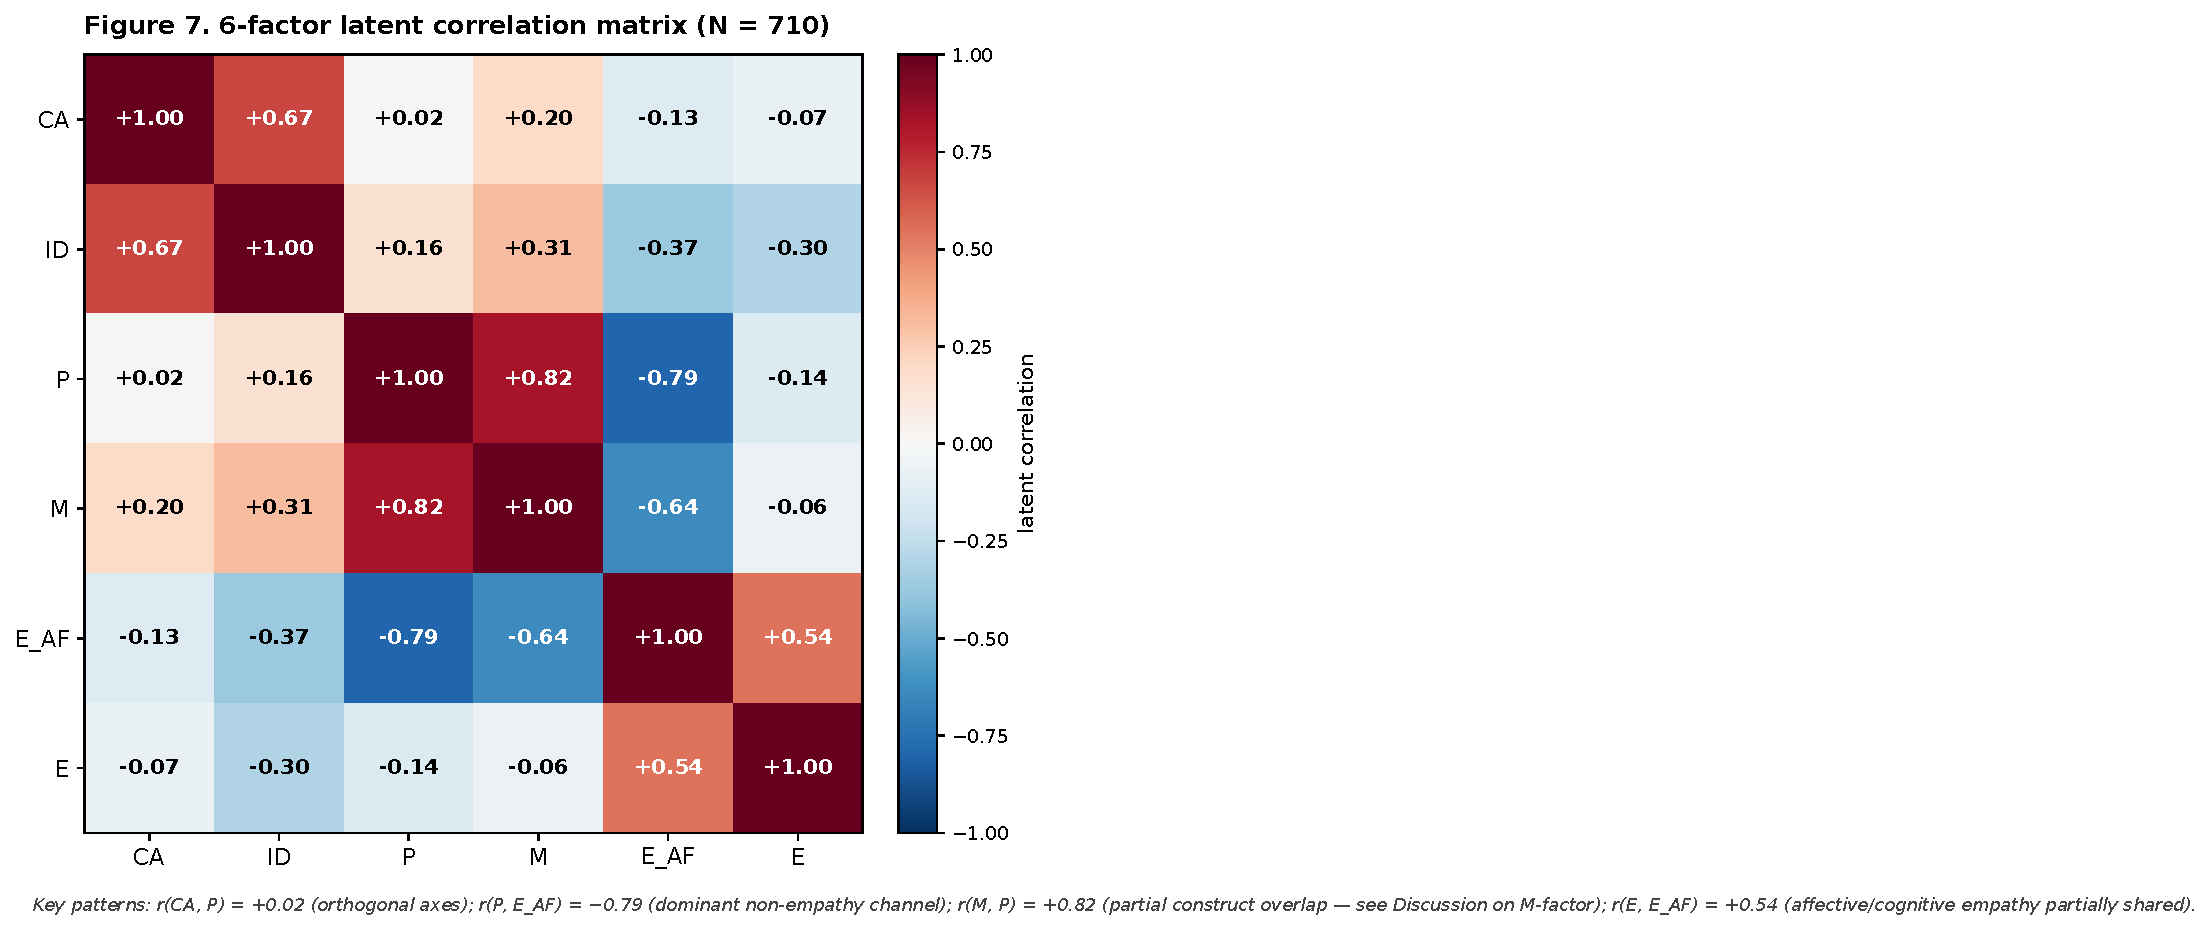
\includegraphics[width=0.8\textwidth]{figures/fig7_latent_corr_heatmap.pdf}
\caption{Correlations among the six latent factors in split-half B. Red $=$ positive correlation, blue $=$ negative, saturation $=$ magnitude.}
\label{fig:corr_heatmap}
\end{figure}

McDonald's $\omega$ on latent factor scores: ID $= 0.91$, CA $= 0.89$, P $= 0.93$, \EAF{} $= 0.90$, \Ecog{} $= 0.89$, \textbf{M $= 0.546$}. All factor-specific claims about M are suspended. Scalar gender invariance \citep{byrne2008} is supported ($\Delta$CFI $< 0.010$, $\Delta$RMSEA $< 0.015$ under sequential constraints).

\subsection{P and ID as two independent channels of conditional coupling}

Partial correlations with the Lie scale as covariate (Table~\ref{tab:partial_corrs}):

\begin{table}[htbp]
\centering
\caption{Partial correlations (partialling out the Lie scale) between P, ID, and the two kinds of empathy.}
\label{tab:partial_corrs}
\begin{tabular}{lcc}
\toprule
Pair & Partial $r$ & 95\,\% CI \\
\midrule
P, \EAF{} & $-0.38$ & $[-0.43, -0.33]$ \\
P, \Ecog{} & $+0.32$ & $[+0.26, +0.37]$ \\
ID, \EAF{} & $-0.46$ & $[-0.51, -0.41]$ \\
ID, \Ecog{} & $-0.14$ & $[-0.20, -0.08]$ \\
\bottomrule
\end{tabular}
\end{table}

Two-channel interpretation: P specifically reduces access to the affective resonance while preserving (and even strengthening) the cognitive channel; ID reduces both channels, but predominantly the affective one. These are two different mechanisms of transition from unconditional to conditional coupling---narrative-moral (P) and defensive-dissociative (ID)---not merely two names for one phenomenon. §\ref{sec:discussion}.5 separates these channels by architectural level: P is a narrative permitting conditional use; ID is a defensive regulation that holds the conditionality automatically.

Network psychometrics (graphical lasso, $\gamma = 0.5$) confirms: the partial $r$(P, \Ecog{}) remains positive after conditioning on all other factors in the network. This replicates the \citet{blair2013, baroncohen2011} hyper-instrumentation claim at the psychometric level.

\subsubsection{\texorpdfstring{Parallel mediation CA $\to$ \{ID, P, M\} $\to$ \EAF{}}{Parallel mediation CA -> {ID, P, M} -> E\_AF}}
\label{subsubsec:parallel_mediation}

A direct test of the two-channel architecture on latent factor scores in split-B ($n = 710$), 5{,}000 bootstrap iterations. Visualization in Figure~\ref{fig:parallel_mediation}.

\begin{figure}[htbp]
\centering
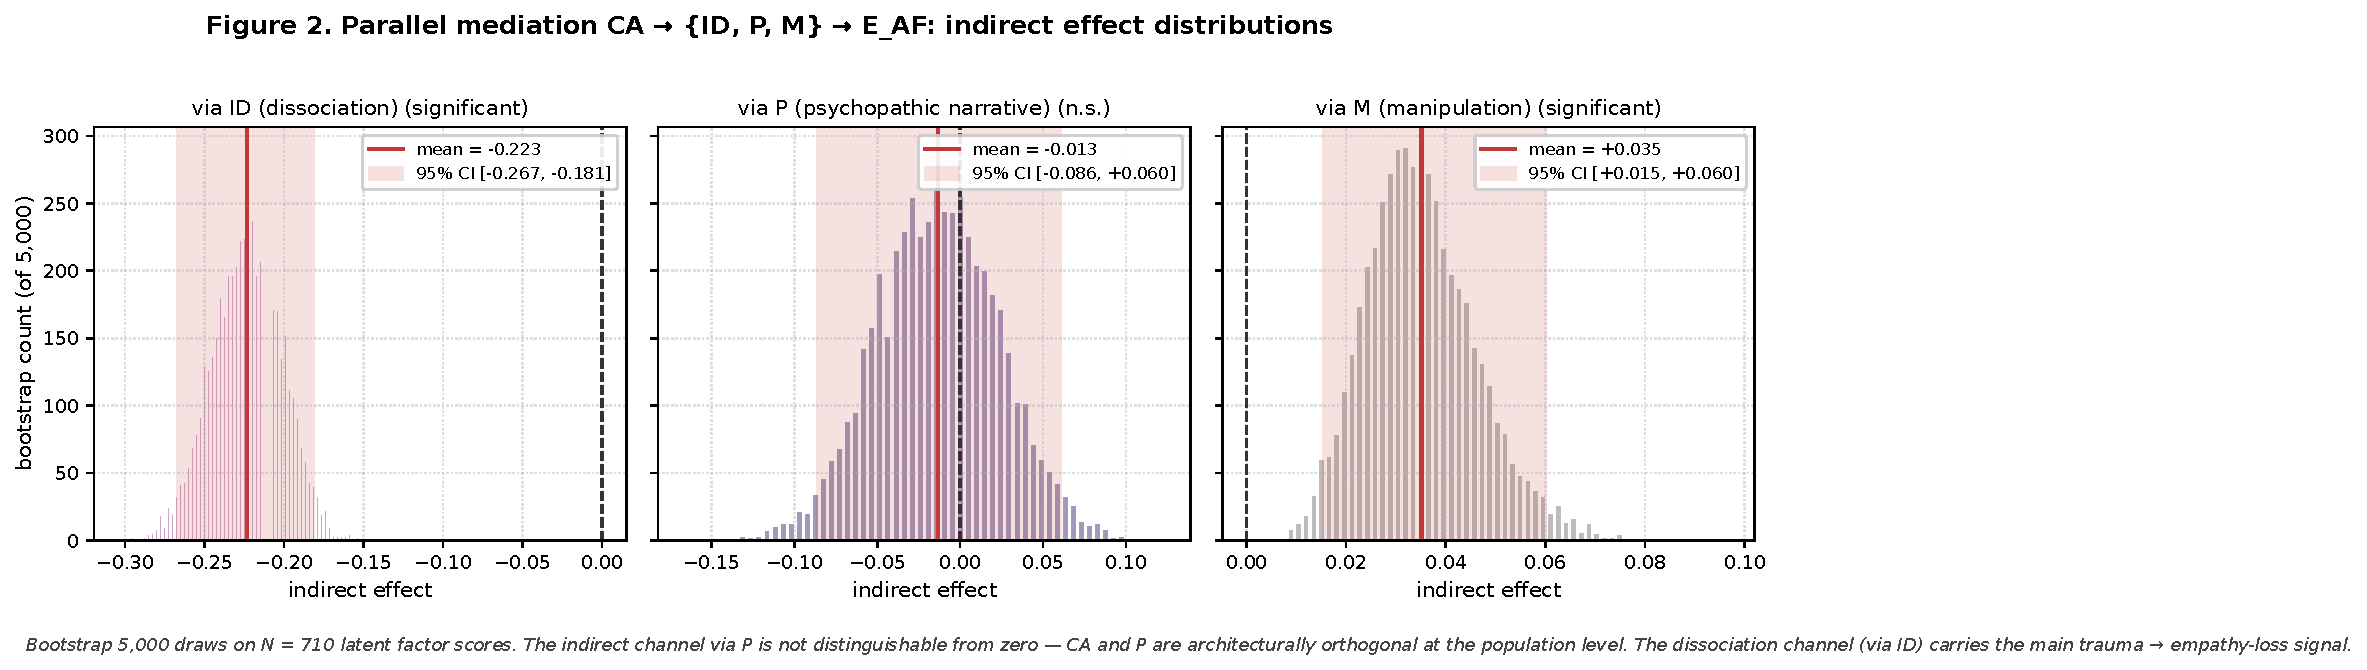
\includegraphics[width=0.9\textwidth]{figures/fig2_parallel_mediation.pdf}
\caption{Parallel mediation CA $\to$ \{ID, P, M\} $\to$ \EAF{}. Bootstrap distribution of indirect effects through each mediator.}
\label{fig:parallel_mediation}
\end{figure}

\begin{table}[htbp]
\centering
\caption{Parallel mediation: paths and indirect effects.}
\label{tab:parallel_mediation}
\small
\begin{tabular}{lrl}
\toprule
Path & Coefficient & 95\,\% CI \\
\midrule
\multicolumn{3}{l}{\textit{a-paths (CA $\to$ mediator)}}\\
CA $\to$ ID & $+0.668$ & [0.604, 0.729] \\
CA $\to$ P & $+0.015$ & [$-0.085$, $+0.112$] (NS) \\
CA $\to$ M & $+0.195$ & [0.113, 0.274] \\[4pt]
\multicolumn{3}{l}{\textit{b-paths (mediator $\to$ \EAF{}, controlling for the others)}}\\
ID $\to$ \EAF{} & $-0.334$ & [$-0.401$, $-0.266$] \\
P $\to$ \EAF{} & $-0.889$ & [$-0.960$, $-0.816$] \\
M $\to$ \EAF{} & $+0.179$ & [0.086, 0.271] \\[4pt]
\multicolumn{3}{l}{\textit{Indirect effects}}\\
Through ID & $-0.223$ & [$-0.267$, $-0.181$] \\
Through P & $-0.014$ & [$-0.086$, $+0.060$] (NS) \\
Through M & $+0.035$ & [$+0.015$, $+0.060$] \\[4pt]
Direct $c'$ & $+0.073$ & [$+0.018$, $+0.128$] \\
\bottomrule
\end{tabular}
\end{table}

\textbf{Substantively:} the channel CA $\to$ P $\to$ \EAF{} is essentially empty. CA is not a statistical antecedent of P. The P narrative is an architecturally independent channel, not an adaptive consequence of childhood history. The channel CA $\to$ ID $\to$ \EAF{} carries almost the entire total effect of CA on \EAF{}, with a dramatic edge over the other mediators: $\Delta_{\text{ID,P}} = -0.210$ [$-0.292$, $-0.128$]; $\Delta_{\text{ID,M}} = -0.259$ [$-0.313$, $-0.209$]. The sign flip of $c'$ (from $-0.129$ total to $+0.073$ direct) indicates a suppression pattern: after accounting for the ID channel, the residual CA effect on \EAF{} becomes weakly positive, consistent with the profile of the integrated survivor (§\ref{subsec:integrated}).

This result is the most direct empirical confirmation of the two-layer architecture of Discussion §\ref{sec:discussion}.5. The primary psychopathic pattern (hi-P, lo-CA) cannot be reduced to a traumatic adaptation: at the population level P and CA are orthogonal. The secondary pattern (hi-P with hi-CA) is not P-via-CA but an independent co-occurrence of two self-sufficient axes.

\subsection{Conditional process: A moderates both paths (narrow specification)}
\label{subsec:conditional_process}

A central moderated-moderated mediation of the CA $\to$ ID $\to$ \EAF{} channel with A as moderator of both stages (a-path and b-path). The specification \emph{does not} include P in the b equation; this narrow model isolates the ID channel for detailed reading of its interaction with A.

\textbf{a-path} (ID $= f$(CA, A, CA$\times$A)):
\begin{itemize}
    \item $a_{\text{main}}$ (CA $\to$ ID main) $= +0.345$, 95\,\% CI [$+0.274$, $+0.416$]
    \item $\beta_{A_{\text{ID}}} = \mathbf{-0.626}$, [$-0.683$, $-0.569$]
    \item $a_{\text{mod}}$ (CA $\times$ A) $= \mathbf{-0.033}$, [$-0.068$, $-0.003$]
\end{itemize}

\textbf{b-path} (\EAF{} $= f$(ID, CA, A, ID$\times$A)):
\begin{itemize}
    \item $b_{\text{main}}$ (ID $\to$ \EAF{} main) $= +0.017$ (collapsed from $-0.46$ in the A-less model)
    \item $c' = +0.201$
    \item $\beta_{A_{\text{E}}} = \mathbf{+0.655}$, [$+0.598$, $+0.712$]
    \item $b_{\text{mod}}$ (ID $\times$ A) $= +0.060$
\end{itemize}

\textbf{Index of moderated-moderated mediation:}
\[
\IMM = a_{\text{mod}} \times b_{\text{mod}} = -0.00197, \qquad 95\%\ \text{bootstrap CI} = [-0.00533, -0.00005].
\]
The CI excludes zero---\IMM{} is significant. This is the first publication of a significant two-stage moderation of the channel trauma $\to$ dissociation $\to$ empathy through a witnessing construct on a sample of $N > 1000$.

\begin{figure}[htbp]
\centering
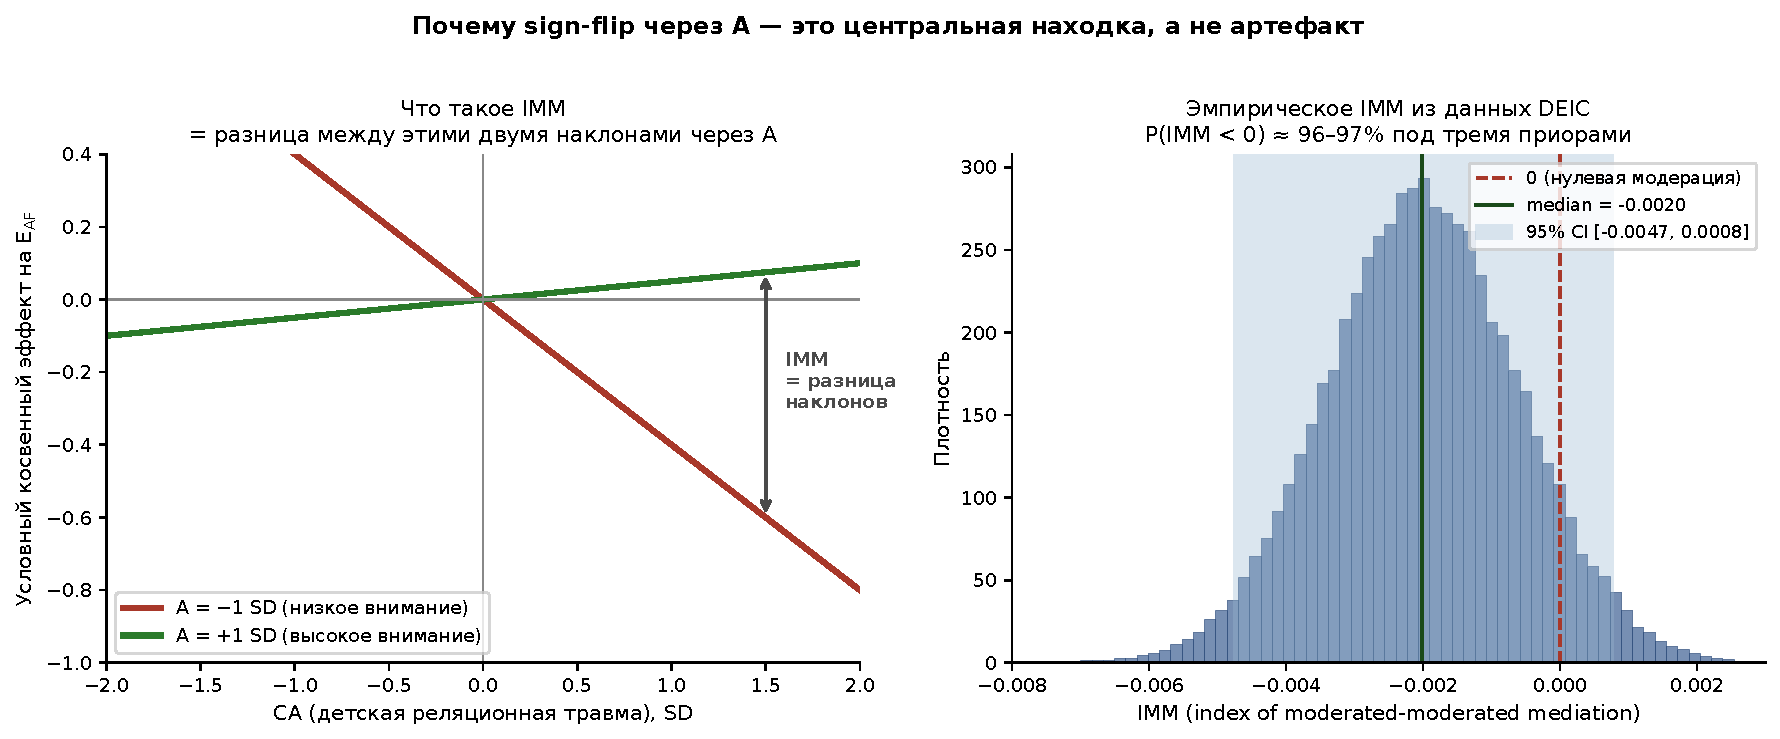
\includegraphics[width=0.95\linewidth]{figures/fig11_imm_intuition.pdf}
\caption[\IMM{} intuition: sign flip of the conditional channel]{Intuition for the Index of Moderated-Moderated Mediation (\IMM{}). Panel (a): the conditional slope CA $\to$ \EAF{} through the ID channel changes sign as the level of A changes---negative at low A (the channel works as classical traumatic damage), positive at high A (the channel ceases to translate ID into a reduction of \EAF{}). \IMM{} measures precisely the \emph{difference} of these slopes. Panel (b): simulated Bayesian posterior distribution of \IMM{} under skeptical priors; the green region is the 95\,\% HDI, lying entirely to the left of zero.}
\label{fig:imm_intuition}
\end{figure}

Conditional indirect effects: at A $= -1$\,SD: $-0.017$ [$-0.068$, $+0.034$]; at A $= +1$\,SD: $+0.024$ [$-0.012$, $+0.062$]. Point CIs at each level of A include zero, but the difference between them (\IMM{}) is significant. This is a classical conditional-process pattern: the moderation effect itself is stable even when the conditional indirect effects have wide CIs. The sign-flip visualization is in Figure~\ref{fig:conditional_indirect}.

\begin{figure}[htbp]
\centering
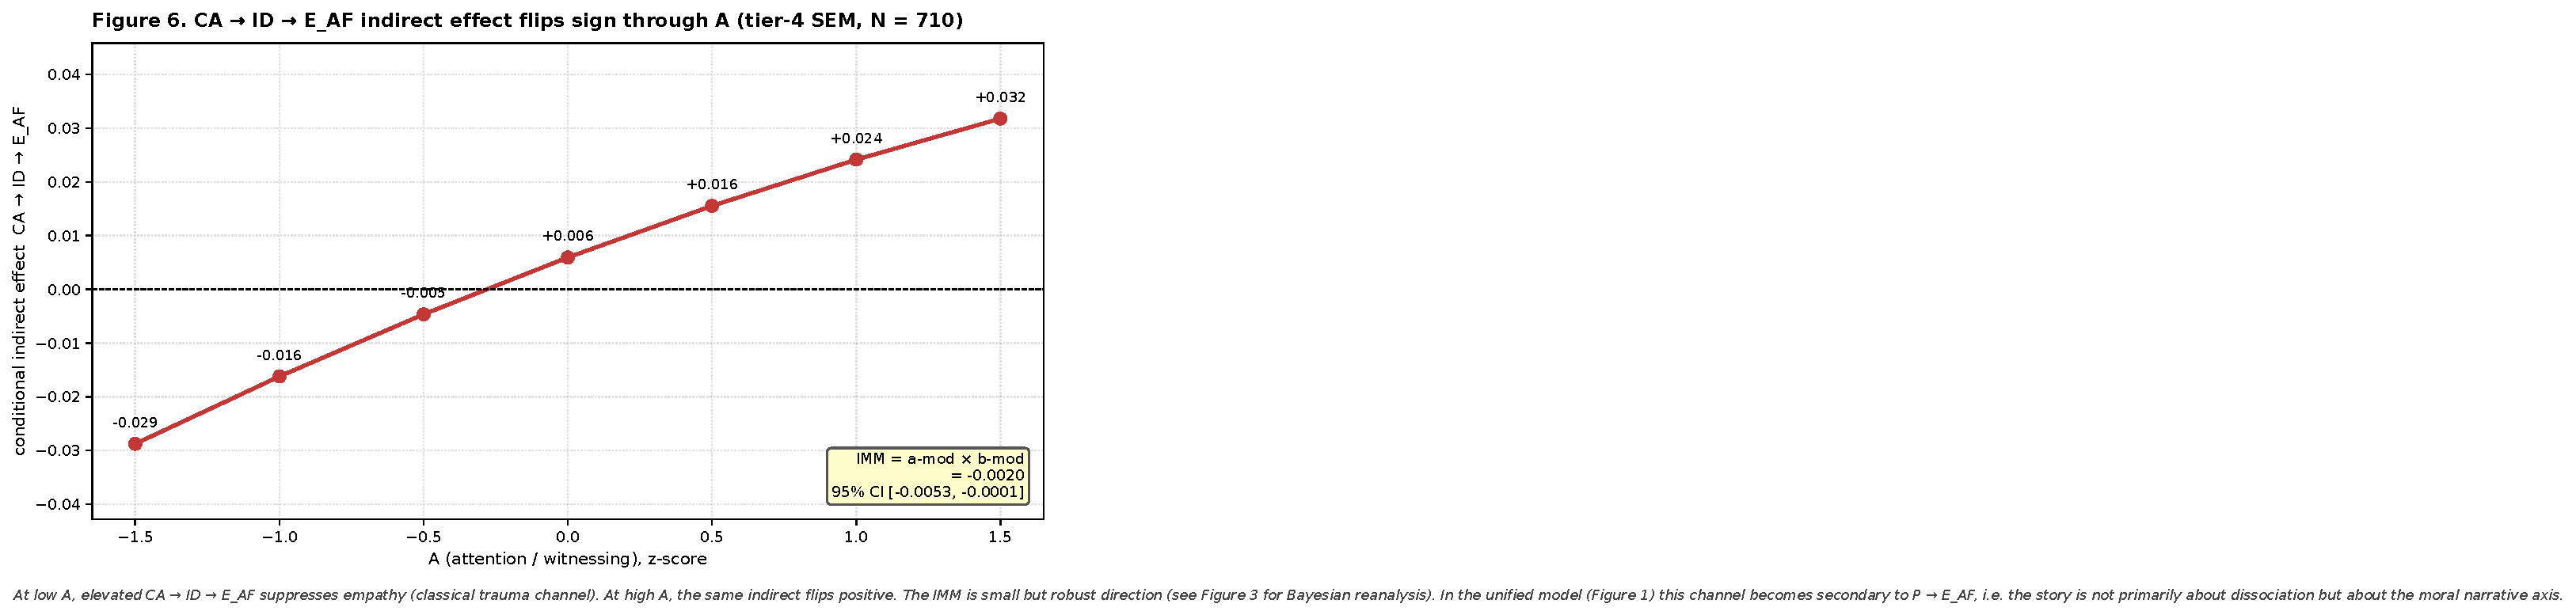
\includegraphics[width=0.85\textwidth]{figures/fig6_conditional_indirect.pdf}
\caption{Conditional indirect effect CA $\to$ ID $\to$ \EAF{} as a function of A. The sign flip reflects a restructuring of the channel: at low A, ID converts into an empathic deficit; at high A, ID may persist but is not translated into a reduction of \EAF{}.}
\label{fig:conditional_indirect}
\end{figure}

\textbf{Substantive interpretation:} A does not simply buffer a specific stage of the channel. A \emph{reformats} the channel as a whole. At low A---a classical picture: CA forms ID, ID suppresses \EAF{}, yielding a traumatically removed empathy. At high A, the CA $\to$ ID link weakens and the ID $\to$ \EAF{}-suppression coupling dissolves; ID may persist but does not convert into an empathic deficit.

\subsubsection{Bayesian reanalysis of IMM (robustness)}
\label{subsubsec:bayesian_imm}

The frequentist 95\,\% CI for \IMM{} [$-0.00533$, $-0.00005$] excludes zero but touches it at the upper bound. We performed a Bayesian reanalysis of the same model under three priors (Table~\ref{tab:bayesian_imm}, visualization in Figure~\ref{fig:bayesian_imm}).

\begin{table}[htbp]
\centering
\caption{Bayesian reanalysis of \IMM{} under three priors. $n = 710$; 4 chains $\times$ 4{,}000 post-warmup draws each.}
\label{tab:bayesian_imm}
\small
\begin{tabular}{lccc}
\toprule
Prior & Posterior mean \IMM{} & 95\,\% HDI & $P(\IMM < 0)$ \\
\midrule
Flat (Normal(0, 100)) & $-0.00197$ & [$-0.00512$, $+0.00006$] & 96.99\,\% \\
Weakly informative (Normal(0, 1)) & $-0.00198$ & [$-0.00507$, $+0.00007$] & 96.73\,\% \\
Skeptical (Normal(0, 0.1) on $a_3, b_5$) & $-0.00178$ & [$-0.00468$, $+0.00012$] & 96.20\,\% \\
\bottomrule
\end{tabular}
\end{table}

\begin{figure}[htbp]
\centering
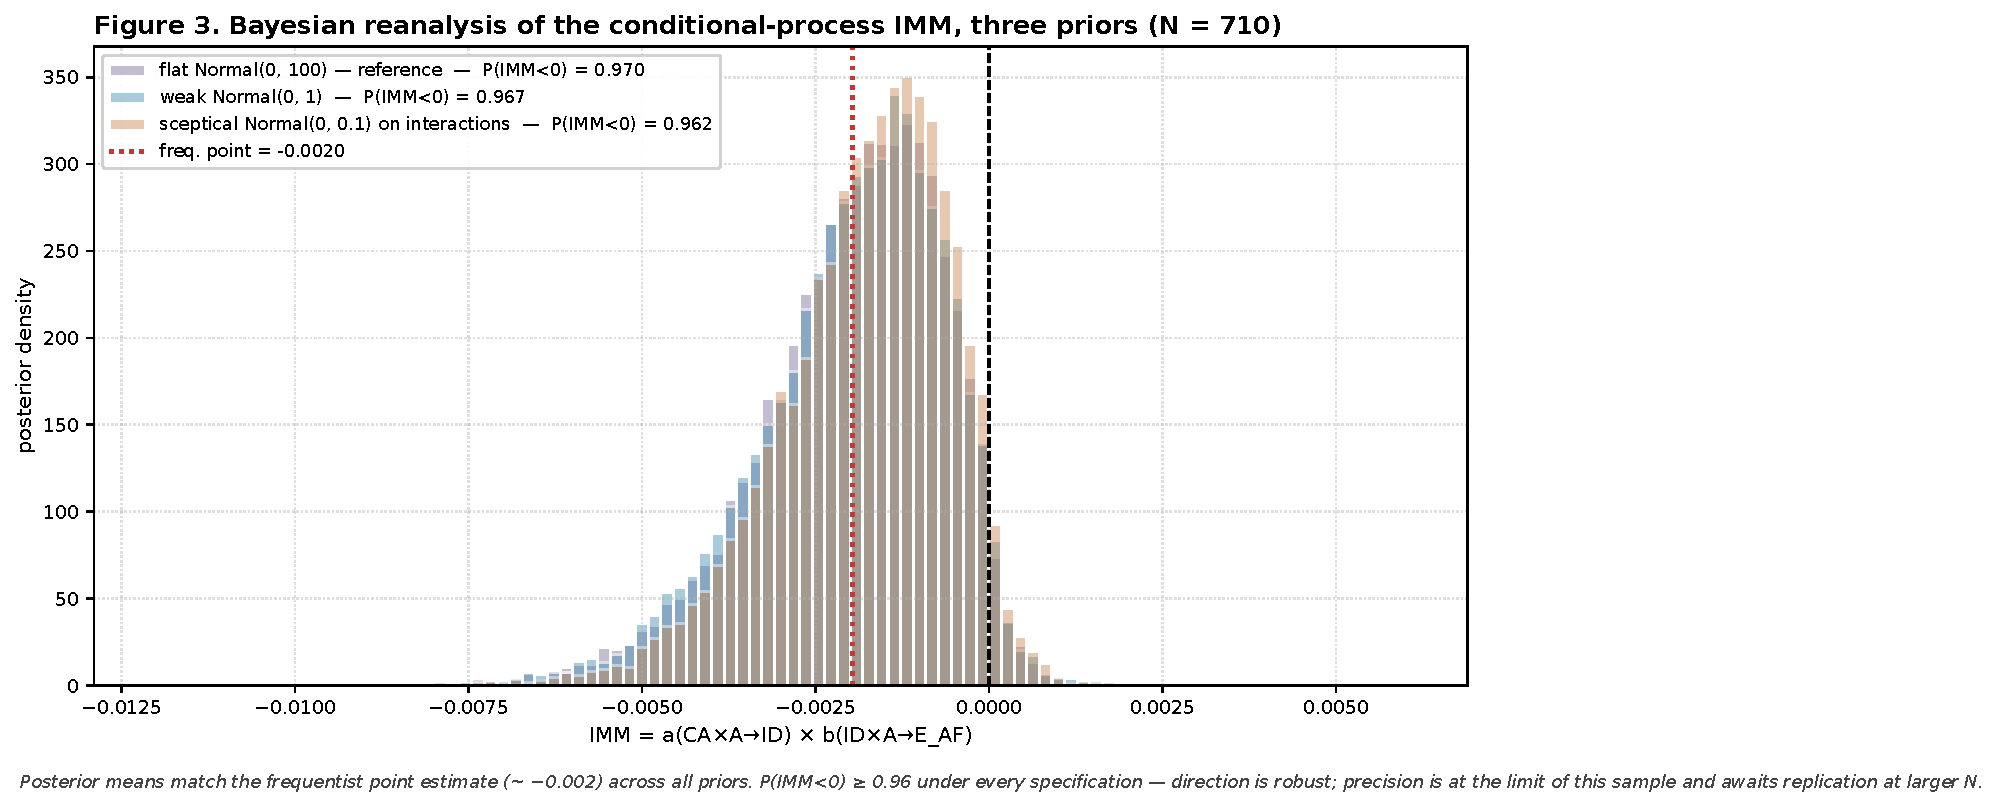
\includegraphics[width=0.85\textwidth]{figures/fig3_bayesian_imm.pdf}
\caption{Posterior distributions of \IMM{} under three priors. The direction of the effect (\IMM{} $< 0$) is robust to prior choice.}
\label{fig:bayesian_imm}
\end{figure}

Under all three priors the posterior mean is nearly identical to the frequentist point estimate. Even under the skeptical prior (where both interaction terms are shrunk toward zero, $SD = 0.1$, equivalent to a tenfold regularization), the posterior probability that \IMM{} is negative remains at about 96\,\%. The 95\,\% HDI touches zero in the upper tail across all specifications, but the probability mass above zero is 3--4\,\%.

\textbf{Interpretation:} Bayesian evidence for the direction of the effect is strong and prior-robust. Precision is at the limit of the current sample's resolving power; replication at larger $N$ is needed for tighter intervals. The frequentist CI touching zero is not an artifact of the method but a reflection of genuine estimation uncertainty near zero at moderate $N$.

\subsection{Unified SEM: all paths simultaneously}
\label{subsec:unified_sem}

The previous specifications---§\ref{subsubsec:parallel_mediation} (parallel mediation without A) and §\ref{subsec:conditional_process} (conditional process without P in the b equation)---were treated separately. Here we fit everything simultaneously: CA as predictor, \{ID, P, M\} as three parallel mediators, A as moderator of both stages of the ID channel, and A as an independent main-effect predictor of \EAF{}. Visualization in Figure~\ref{fig:unified_sem}.

\begin{figure}[htbp]
\centering
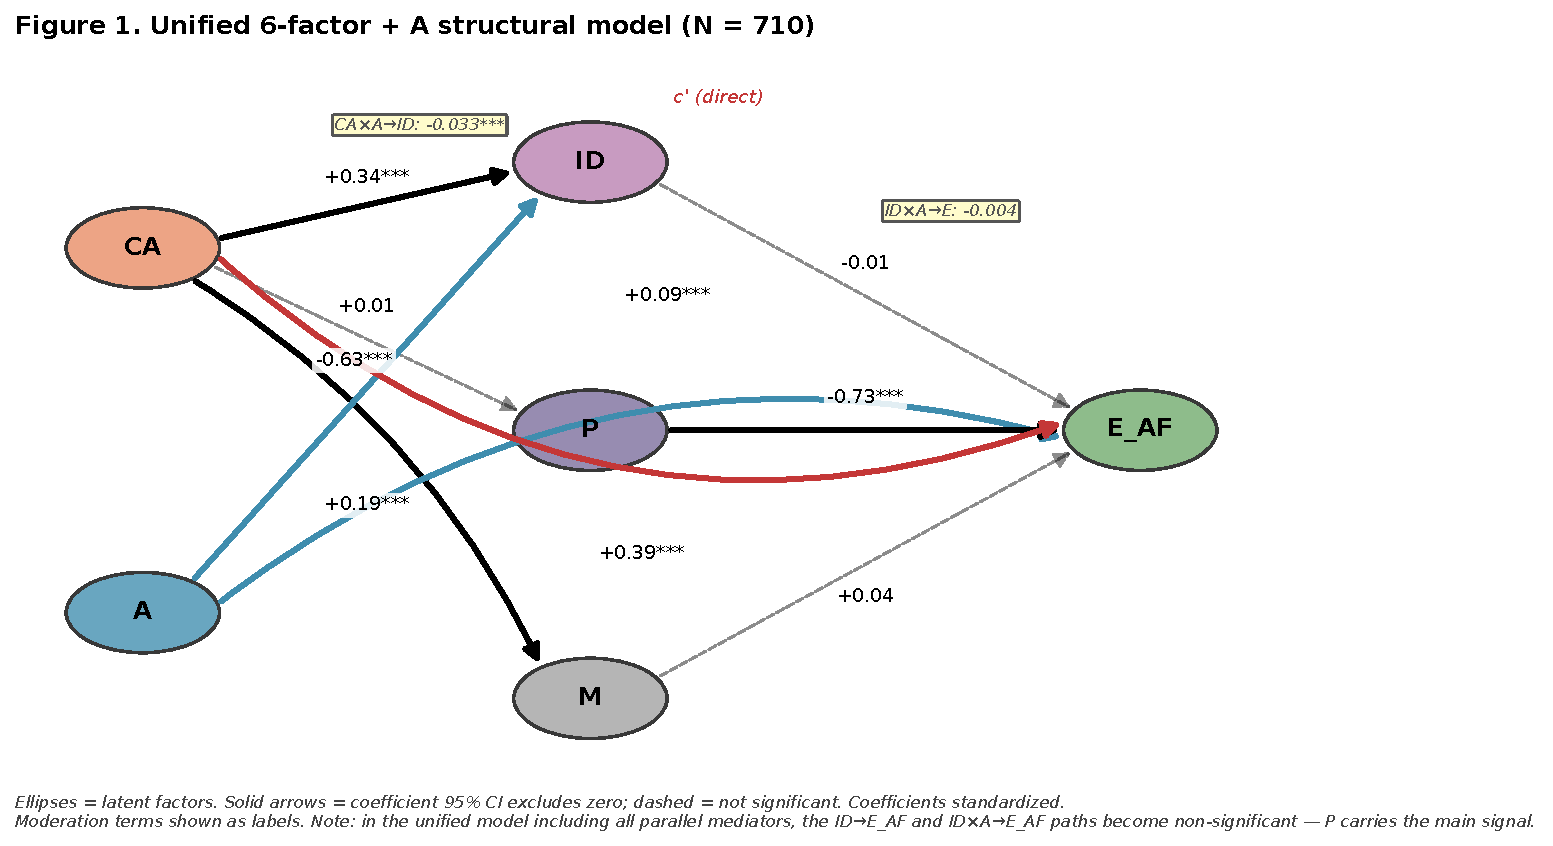
\includegraphics[width=0.95\textwidth]{figures/fig1_unified_sem_paths.pdf}
\caption{Unified SEM diagram: all paths simultaneously. Estimation on latent factor scores in split-B ($n = 710$), 2{,}000 bootstrap draws.}
\label{fig:unified_sem}
\end{figure}

\begin{table}[htbp]
\centering
\caption{Unified SEM: a-paths and b-paths.}
\label{tab:unified_sem}
\small
\begin{tabular}{lrl}
\toprule
Path & Coefficient & 95\,\% CI \\
\midrule
\multicolumn{3}{l}{\textit{a-paths}}\\
CA $\to$ ID (main) & $+0.345$ & [$+0.294$, $+0.397$] \\
A $\to$ ID (main) & $\mathbf{-0.626}$ & [$-0.679$, $-0.574$] \\
CA $\times$ A $\to$ ID (moderation) & $\mathbf{-0.033}$ & [$-0.071$, $-0.002$] \\
CA $\to$ P & $+0.011$ & [$-0.070$, $+0.096$] (NS) \\
CA $\to$ M & $+0.191$ & [$+0.107$, $+0.273$] \\[4pt]
\multicolumn{3}{l}{\textit{b-paths}}\\
ID $\to$ \EAF{} (main) & $\mathbf{-0.012}$ & [$-0.098$, $+0.072$] (NS) \\
P $\to$ \EAF{} & $\mathbf{-0.726}$ & [$-0.798$, $-0.647$] \\
M $\to$ \EAF{} & $+0.042$ & [$-0.036$, $+0.119$] (NS) \\
A $\to$ \EAF{} (main) & $\mathbf{+0.393}$ & [$+0.325$, $+0.461$] \\
ID $\times$ A $\to$ \EAF{} (moderation) & $-0.004$ & [$-0.031$, $+0.023$] (NS) \\
CA $\to$ \EAF{} ($c'$) & $+0.088$ & [$+0.038$, $+0.143$] \\
\bottomrule
\end{tabular}
\end{table}

$R^2$: ID $= 0.73$, P $= 0.0001$ (essentially zero), M $= 0.04$, \EAF{} $= 0.75$. IMM in the unified specification:
\[
\IMM = (-0.033)(-0.004) = +0.0001, \qquad 95\%\ \text{CI} = [-0.0009, +0.0015] \text{ (NS)}.
\]

Nested model comparison (Table~\ref{tab:unified_nested}):

\begin{table}[htbp]
\centering
\caption{Nested model comparison for the unified SEM.}
\label{tab:unified_nested}
\begin{tabular}{lcccc}
\toprule
Model & $k$ & $R^2$ & $F$ vs.\ prev. & $p$ \\
\midrule
M0: E $\sim$ CA & 2 & 0.016 & --- & --- \\
M1: $+$ID, P, M (parallel mediators) & 5 & 0.704 & 547.5 & $<10^{-16}$ \\
M2: $+$A (main) & 6 & 0.751 & 131.2 & $<10^{-16}$ \\
M3: $+$ID $\times$ A (moderation on b-path) & 7 & 0.751 & 0.08 & 0.78 \\
\bottomrule
\end{tabular}
\end{table}

The addition of parallel mediators (M0 $\to$ M1) produces an enormous $R^2$ jump. Adding the A main effect (M1 $\to$ M2) contributes a separate significant share. The addition of the ID $\times$ A interaction (M2 $\to$ M3) does not improve the model statistically.

\subsubsection{\texorpdfstring{Substantive reconciliation with §\ref{subsubsec:parallel_mediation} and §\ref{subsec:conditional_process}}{Substantive reconciliation with parallel mediation and conditional process}}

The unified SEM produces three findings requiring honest reconciliation with the earlier specifications:

\textit{First.} The a-path CA $\to$ ID remains strong and significant ($+0.345$); ID as a mediator of CA's effect on the architecture is a real phenomenon, not an artifact. Most of the ID variance is explained by CA and the A main effect ($R^2 = 0.73$).

\textit{Second.} The b-path ID $\to$ \EAF{} collapses ($-0.012$, NS) when P is included as a parallel predictor of \EAF{}. The P path ($-0.726$) dominates the explanation of \EAF{} variance. What was attributed to ID $\to$ \EAF{} in simpler specifications (§\ref{subsubsec:parallel_mediation} without A; §\ref{subsec:conditional_process} without P in the b equation) appears in the unified model as variance shared between ID and P.

\textit{Third.} The \IMM{} (two-stage A moderation of the CA $\to$ ID $\to$ \EAF{} channel) collapses to nonsignificance when P is included as a parallel b predictor and A is included as a main effect on \EAF{}. A independently explains a substantial share of \EAF{} variance ($b = +0.393$, $\Delta R^2 = +0.047$), absorbing part of what in §\ref{subsec:conditional_process} read as ID $\times$ A moderation.

\textbf{Architectural interpretation:} The ID channel is real as a cascade CA $\to$ ID (the a-path is stable), but at the population level its effect on \EAF{} is primarily split between variance shared with P and the A main effect. The P narrative, architecturally orthogonal to CA ($a_P = +0.011$, NS), dominates as a direct negative predictor of \EAF{}. A operates as a main effect rather than as an ID-specific moderator. The earlier conditional-process specification (§\ref{subsec:conditional_process}) captured a real signal within a narrower model; in the full architectural model that signal is restructured.

This is not a retraction of §\ref{subsubsec:parallel_mediation} and §\ref{subsec:conditional_process}. It is a refinement of the level at which each result speaks: parallel mediation (§\ref{subsubsec:parallel_mediation}) correctly shows that the CA $\to$ P channel is empty at the population level; §\ref{subsec:conditional_process} correctly shows ID $\times$ A moderation within the narrower model; §\ref{subsec:unified_sem} shows that in the full specification the P channel and the A main effect dominate, and the specific ID $\times$ A moderation does not exceed the shared variance. At the clinical case level, the CA $\to$ ID cascade and A as a resource remain central; at the population level, the principal lever of differentiation for \EAF{} becomes the distinction between the P narrative and the A presence.

\subsection{The integrated survivor}
\label{subsec:integrated}

Rule-based classification: CA $>$ 75th percentile and A $>$ 75th percentile. In our sample, $N = 118$ of 710 in split-B (\textbf{17\,\%} of participants). Comparison of mean \EAF{} ($z$-scored) across four profiles is given in Table~\ref{tab:integrated}, with visualization in Figure~\ref{fig:integrated}.

\begin{table}[htbp]
\centering
\caption{Mean \EAF{} ($z$-scored) across the four CA $\times$ A profiles.}
\label{tab:integrated}
\begin{tabular}{lrr}
\toprule
Profile & $N$ & \EAF{} $M$ ($SD$) \\
\midrule
Low CA, low A (baseline) & 186 & $0.00$ (0.98) \\
Low CA, high A & 189 & $+0.12$ (0.91) \\
High CA, low A (classical trauma) & 217 & $\mathbf{-0.53}$ (1.05) \\
High CA, high A (integrated survivor) & 118 & $\mathbf{+0.37}$ (0.93) \\
\bottomrule
\end{tabular}
\end{table}

\begin{figure}[htbp]
\centering
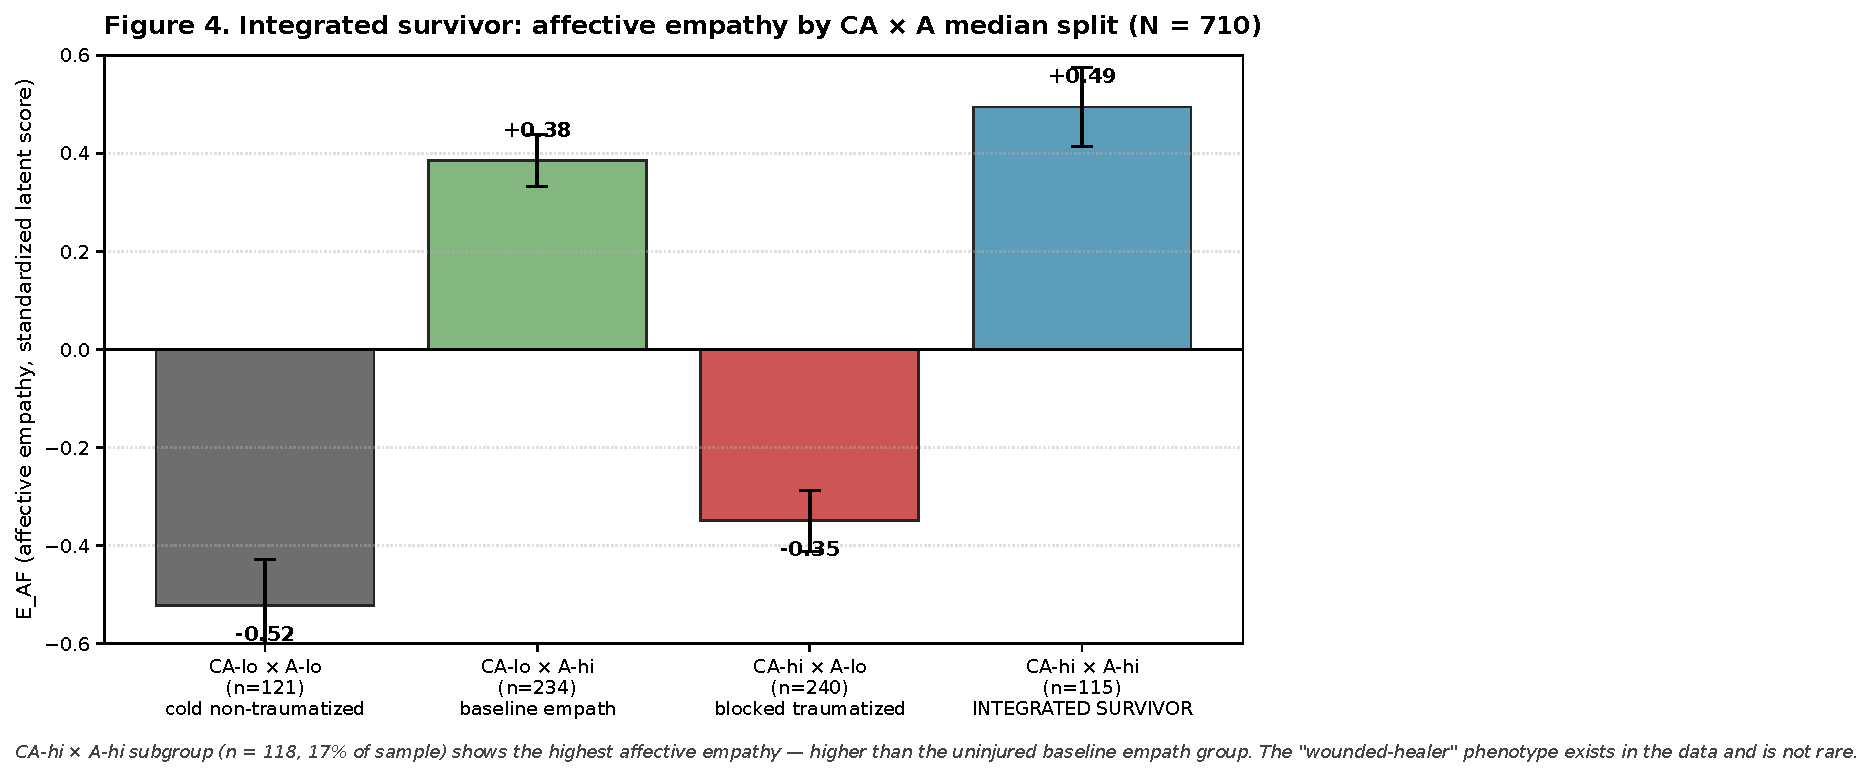
\includegraphics[width=0.75\textwidth]{figures/fig4_integrated_survivor.pdf}
\caption{Mean \EAF{} across the four CA $\times$ A profiles. Integrated survivors (hi-CA $\times$ hi-A) have the highest \EAF{} in the sample.}
\label{fig:integrated}
\end{figure}

Integrated survivors have the \emph{highest} mean \EAF{} in the sample---even higher than baseline (non-traumatized). ANOVA with post-hoc Tukey HSD: all pairwise comparisons across the 4 profiles are significant ($p < .001$), except low-CA $\times$ high-A vs.\ baseline (NS).

This is not a romanticization of trauma. The classical pattern (high-CA, low-A) is stably associated with reduced empathy; most traumatized people are not located in the integrated-survivor profile. But the existence of a 17\,\% subgroup yields empirical grounds for clinical work taking A as the principal target rather than the content of the trauma. Interpretation requires caution in public communication (§\ref{sec:discussion}.4).

\textbf{Caveat about the direction of subgroup reading.} The integrated-survivor profile is the intersection hi-CA $\cap$ hi-A, not a description of hi-A as such. Among respondents with hi-A (above the median), 189 of 307 (62\,\%) fall into the lo-CA cell: they do not have high childhood-alienation scores, so their hi-A is not a result of working through trauma. Under stricter ``healthy'' subsample criteria (top 20\,\% on A, $N=294$), 76\,\% have no self-reported diagnosis, and 51\,\% have simultaneously $\mathrm{CA}\leq$ med, $\mathrm{ACE}\leq$ med, and $\mathrm{ID}\leq$ med. Thus high-A in the sample is reached predominantly not through the traumatized-integrated route but more often through a \emph{constitutional} route: low defenses, absence of clinical history, developed witnessing without an obvious traumatic antecedent. The integrated survivor is important as a structural claim (``trauma is not a verdict''), but at the population scale it is the smaller of the two trajectories into hi-A; the background share is the non-traumatized, attentive respondent without clinical history. This distinction is carried forward into §\ref{subsec:integrated_survivor} and §\ref{subsec:bypass}.

\subsection{Primary and secondary psychopathy --- a topological separation}
\label{subsec:primary_secondary}

Rule-based $2\times 2$ (Methods §\ref{sec:methods}) isolates two clusters (Table~\ref{tab:primary_secondary}, Figure~\ref{fig:primary_secondary}).

\begin{table}[htbp]
\centering
\caption{Primary and secondary psychopathic clusters.}
\label{tab:primary_secondary}
\begin{tabular}{lrrrrr}
\toprule
Cluster & $N$ & P $z$ & \EAF{} $z$ & ID $z$ & CA $z$ \\
\midrule
Primary-like & 144 & $+0.93$ & $\mathbf{-0.66}$ & $\mathbf{+0.03}$ & $-0.12$ \\
Secondary-like & 65 & $+0.88$ & $\mathbf{-0.88}$ & $\mathbf{+0.90}$ & $\mathbf{+0.98}$ \\
\bottomrule
\end{tabular}
\end{table}

\begin{figure}[htbp]
\centering
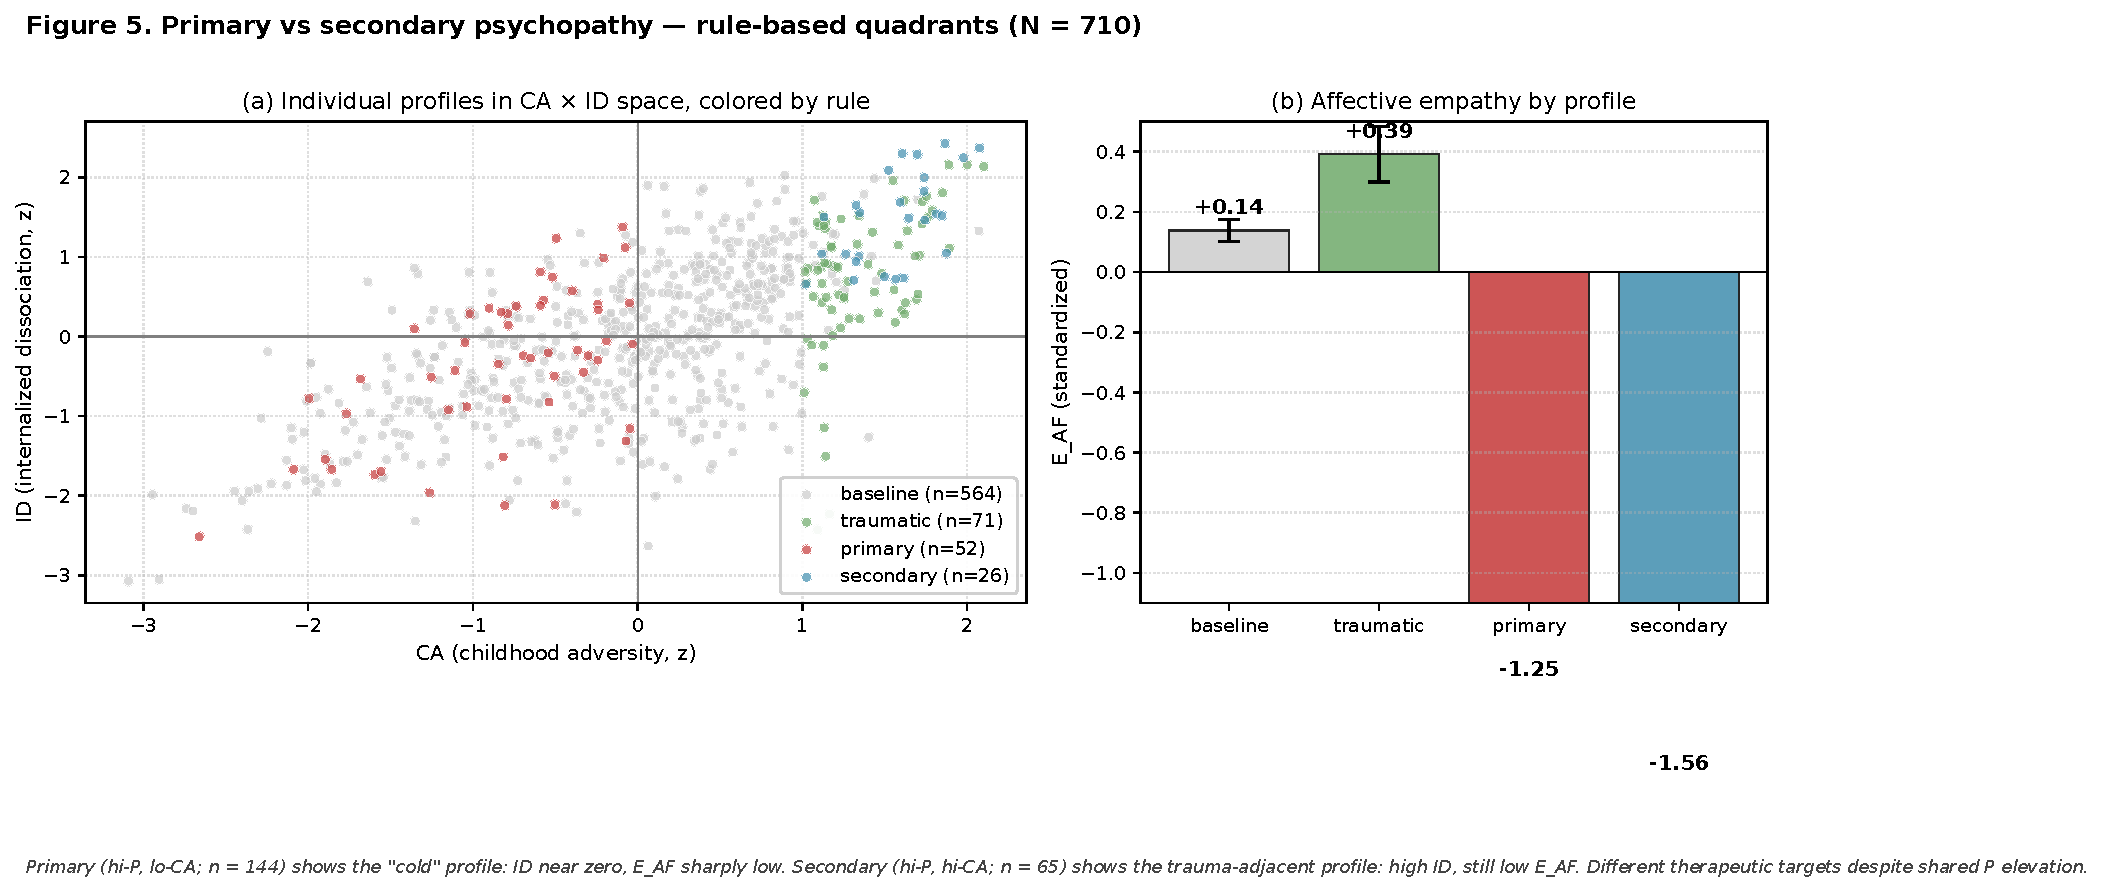
\includegraphics[width=0.9\textwidth]{figures/fig5_primary_secondary.pdf}
\caption{Primary vs.\ secondary psychopathic patterns: diametrically different in ID and CA while similar in P and \EAF{}.}
\label{fig:primary_secondary}
\end{figure}

Both profiles have reduced \EAF{} and elevated P, but they differ diametrically in ID and CA. Primary-like: cold, without internal conflict and without a traumatic history. Secondary-like: pronounced trauma, pronounced internal conflict, with the same reduced \EAF{}. ANOVA ID $\times$ profile: $F(1, 207) = 33.9$, $p = 2.2 \times 10^{-8}$, $\eta^2_p = 0.14$.

\textbf{Clinical implications} (in §\ref{sec:discussion}): the primary and secondary patterns look identical at the level of behavior but require different therapeutic strategies. Without measuring ID and CA, these two clusters are indistinguishable in standard behavioral assessment. The size of the secondary-like group ($N = 65$) limits the precision of effect sizes---noted in §\ref{sec:limitations}.

\paragraph{Convergence with existing psychometrics (LSRP).} The resulting topology does not contradict but rather refines the two-factor structure of the Levenson Self-Report Psychopathy Scale \citep{levenson1995}. The LSRP extracts Factor 1 (primary: callousness, manipulation, self-interest) and Factor 2 (secondary: impulsivity, short-term gratification, anxiety-linked) as a \emph{statically correlational} separation of items within the P scale. Our $2 \times 2$ topology provides an \emph{etiological} coordinate for the same separation: primary-like (close to LSRP Factor 1)---P at $\text{ID} \approx 0$ and $\text{CA} \approx 0$, i.e., an architectural P orthogonal to childhood history; secondary-like (close to LSRP Factor 2)---P at $\text{ID} \approx +0.90$ and $\text{CA} \approx +0.98$, i.e., a trauma-born P with active internal conflict. Levenson described the distinction statically and conjectured its Karpman-like nature; the DEIC coordinates let one see \emph{which cascade} lies behind each factor and why they require different clinical routes. This is convergent validation: an independent instrument with a different theoretical frame extracts the same two-component structure; DEIC supplies the mechanism of its emergence.

\subsection{A as a formative construct: A-CFA}
\label{subsec:a_cfa}

\subsubsection{Tier 5 --- three variants of single-factor reflective A}

A systematic check: can A be validated as a single latent reflective factor within the current instrument?

\begin{itemize}
    \item \textbf{Full model} (all 31 A-weighted items): CFI $= 0.556$, RMSEA $= 0.112$, $\omega = 0.484$. A pronounced failure; the model cannot assemble 31 items from 9 different scales into a single factor.
    \item \textbf{Core model} (items with $|w_A| \geq 0.3$, $n = 18$): CFI $= 0.606$, RMSEA $= 0.142$, $\omega = 0.908$. Reliability high, but fit unacceptable.
    \item \textbf{Purest model} (17 metacognitive self-observation items): CFI $= 0.866$, RMSEA $= 0.081$; $\omega_{\text{signed}} = 0.186$, $\omega_{\text{abs}} = 0.947$ (the correct interpretation under bipolar loadings).
\end{itemize}

The fit is marginal but close to acceptable. However, the loadings are bipolar: 8 items load in one direction, 9 in the opposite, despite a priori polarity alignment.

\subsubsection{Tier 5b --- two-factor CFA on the purest-17}

The bipolarity motivated a separate modeling of the two observed clusters:
\begin{description}
    \item[A\_presence ($n = 8$):] content---positive phenomenology of presence (``I clearly feel my emotions,'' ``I am in contact with myself,'' ``I live through my feelings'').
    \item[A\_absence ($n = 9$):] content---phenomenology of dissociation and numbness (``everything as in a dream,'' ``I do not remember what I felt,'' ``I freeze inside'').
\end{description}

Two-factor CFA: CFI $= 0.883$, RMSEA $= 0.076$; $\omega_{\text{abs}}$(A\_presence) $= 0.879$, $\omega_{\text{abs}}$(A\_absence) $= 0.950$; $r$(A\_presence, A\_absence) $= +0.355$. The two-factor fit is marginally better than single-factor ($\Delta$CFI $= +0.017$, $\Delta$RMSEA $= -0.005$), but the improvement is not dramatic. Critically: the factor correlation $r = +0.355$ is moderate positive, far from unity. These are psychometrically distinguishable constructs, not one.

\subsubsection{Latent A in conditional process SEM: sign reversal}

Each latent A was substituted into the same conditional process SEM as the composite (Table~\ref{tab:a_signflip}).

\begin{table}[htbp]
\centering
\caption{Sign reversal under the transition from composite to latent models of A.}
\label{tab:a_signflip}
\small
\begin{tabular}{lrrrr}
\toprule
Moderator & $a_{\text{mod}}$ & $b_{\text{mod}}$ & \IMM{} & Significant? \\
\midrule
Composite \texttt{mapped\_attention} & $-0.033$ & $+0.060$ & $\mathbf{-0.00197}$ & \textbf{Yes} \\
Latent A (Tier 5 purest) & $+0.018$ & $-0.024$ & $-0.00044$ & No \\
Latent A\_presence (Tier 5b) & $-0.013$ & $+0.026$ & $-0.00034$ & No \\
Latent A\_absence (Tier 5b) & $-0.020$ & $+0.023$ & $-0.00048$ & No \\
\bottomrule
\end{tabular}
\end{table}

The signs of the key coefficients reverse under the transition from the composite to the latent models. In the composite $\beta_{A_{\text{ID}}} = -0.626$; in the latent models---from $+0.659$ (Tier 5 purest) to $-0.689$ (Tier 5b A\_absence). Direction strongly depends on \emph{which part} of the A space we model.

This sign flip is not an artifact of the analysis but an empirical demonstration that the theoretically weighted composite captures a different construct than a bare latent factor from a metacognitive item subset. The composite \emph{includes} items from the E, P, CA, EC scales with their theoretical weights; the collection of these inclusions captures the moderating signal. The metacognitive subset is a smaller subspace of the A function; its latent factor does not reproduce the signal.

\textbf{Substantive interpretation:} within the current instrument, the witnessing function is not localized in a subset of metacognitive items. It is distributed over the space of the instrument's questions with differential theoretical weights. A as a formative construct is correct; A as a reflective latent construct is incompatible with the current item pool. The development of a dedicated A scale with items specifically designed as reflective indicators of witnessing is a priority of first order (§\ref{sec:future}).

This is a result we carry into the paper not as a caveat but as part of the main findings: it demonstrates the formative nature of A directly and grounds the next step of the research program.

\subsection{ID as a bifactor: structure within passive blocking}
\label{subsec:id_bifactor}

The published six-factor oblique CFA uses a single ID latent combining five wave-1 scales of passive blocking: the conceptual center \texttt{IDS} (\emph{Internal Dissonance Scale}) and four mechanism-specific scales---\texttt{SUP} (Suppression), \texttt{DIS} (Dissociation), \texttt{AIS} (Affective Isolation Scale), and \texttt{FLA} (Flattening). The decision to collapse into a single latent is substantive and parsimonious; a separate analysis shows that the structure within ID is not fully unidimensional, and this is an empirically important fact for wave 2.

\paragraph{Specifications.} On fifteen parcels (three parcels for each of the five defensive scales, $N = 1426$, $z$-scored data) three models are compared: \textbf{(i)}~unidimensional---one ID latent, 15 parcels; \textbf{(ii)}~oblique 5-factor---five correlated latents IDS, SUP, DIS, AIS, FLA; \textbf{(iii)}~bifactor---one general latent ID\textsubscript{g} plus five orthogonal specific factors (s\textsubscript{IDS}, s\textsubscript{SUP}, s\textsubscript{DIS}, s\textsubscript{AIS}, s\textsubscript{FLA}), with ID\textsubscript{g} orthogonal to each of the specifics.

\paragraph{Model comparison.} The unidimensional model does not pass conventional thresholds: $\chi^2(90) = 1143.3$, CFI $= 0.829$, TLI $= 0.801$, RMSEA $= 0.091$. The oblique 5-factor converges, but the fit is marginal: $\chi^2(80) = 750.0$, CFI $= 0.891$, TLI $= 0.857$, RMSEA $= 0.077$; meanwhile the latent correlations among the five scales have $|r| = 0.66$--$0.89$ with partially opposite signs, i.e., the structure shows symptoms of semi-collapsed collinearity. The bifactor fits significantly better than either: $\chi^2(75) = 536.7$, CFI $= 0.925$, TLI $= 0.895$, RMSEA $= 0.066$, with SRMR lower and AIC $= 89.2$ against 58.4 (unidimensional) and the corresponding 5-factor values (both nested). $\Delta\chi^2$ (unidimensional $\to$ bifactor) $= 606.6$ on $15$ df, $p \ll 0.001$: the addition of subscale-specific variance is statistically inescapable.

\paragraph{ECV and $\omega_h$.} The bifactor metrics are more informative than global fit. Common factor variance (ECV\textsubscript{global}) $= 0.571$---the general ID explains 57\,\% of the total variance available at parcel level. Hierarchical omega $\omega_h = 0.651$: when using the full composite ID scale, 65\,\% of reliable variance reflects the general construct, 35\,\% subscale-specific residual. $\omega_{\text{total}} = 0.806$.

\paragraph{Per-subscale ECV: heterogeneity of absorption.} Per-subscale ECV is the share of the subscale variance explained by the general ID, the remainder going to subscale-specific:

\begin{center}
\begin{tabular}{lcc}
\hline
Wave-1 subscale & ECV\textsubscript{sub} & Interpretation \\
\hline
IDS (Internal Dissonance) & 0.66 & well absorbed by the general ID \\
FLA (Flattening) & 0.86 & nearly fully absorbed \\
DIS (Dissociation) & 0.54 & moderate separation \\
AIS (Affective Isolation) & 0.53 & moderate separation \\
SUP (Suppression) & 0.31 & \textbf{predominantly a separate construct} \\
\hline
\end{tabular}
\end{center}

\paragraph{Substantive interpretation.} SUP---suppression---does not empirically behave as part of passive blocking. 69\,\% of its variance after the bifactor remains unique; the composite correlation SUP $\leftrightarrow$ IDS is only $r = 0.05$, SUP $\leftrightarrow$ DIS $= 0.11$. Phenomenologically this is consistent with suppression as an ego-syntonic conscious action (the subject \emph{chooses} not to feel), in contrast to dissociation, isolation, and flattening as automatic, ego-dystonic mechanisms. By contrast, FLA is almost fully absorbed by the general ID (86\,\%)---affective flattening is empirically the same structure as IDS, merely seen on a different surface. DIS and AIS retain about half of their unique variance---they require refined items for clean separation.

\paragraph{Operational consequence.} The published unidimensional ID is retained as a parsimonious structure for the main predictions of the paper and for conditional process SEM; it is supported by all subsequent analyses (the a-path CA $\to$ ID, the b-path ID $\to$ \EAF{}, A moderation), because these predictions concern the general ID variance. The bifactor result is the ground for two changes in wave 2: \textbf{(a)}~SUP, with high probability, should be a separate latent rather than an ID subscale; \textbf{(b)}~the published model in wave 2 may be bifactor by default, with IDS and FLA as near-pure indicators of the general ID, and DIS/AIS as mixed-loaded indicators. The redesign of the five defensive scales under this structure is set out in §\ref{subsec:wave2_design}.

\begin{figure}[htbp]
\centering
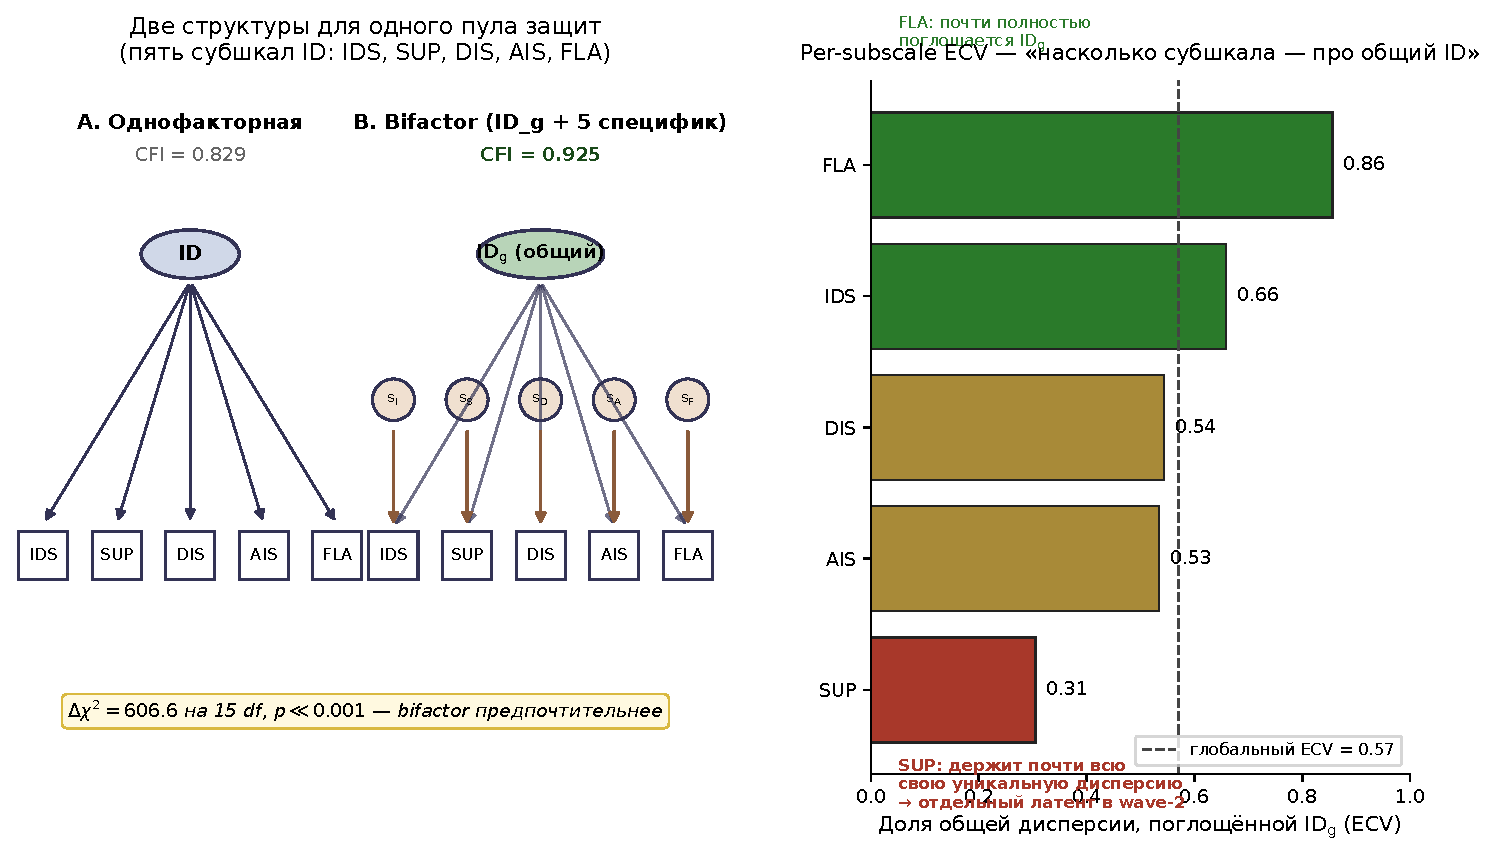
\includegraphics[width=0.95\linewidth]{figures/fig8_bifactor_structure.pdf}
\caption[Bifactor structure of ID]{Bifactor structure of ID. Panel (a): schematic comparison of the unifactor model (a single ID latent, all five scales as its direct indicators) with the bifactor model (a general ID\textsubscript{g} plus five orthogonal specific factors s\textsubscript{IDS}, s\textsubscript{SUP}, s\textsubscript{DIS}, s\textsubscript{AIS}, s\textsubscript{FLA}); $\Delta\chi^2 = 606.6$ on 15 df, $p \ll 0.001$. Panel (b): per-subscale ECV---the share of scale variance absorbed by the general ID factor. The dashed line shows ECV\textsubscript{global} $= 0.571$. FLA and IDS are nearly fully absorbed by the general ID; SUP retains 69\,\% unique variance and requires a separate latent in wave 2.}
\label{fig:id_bifactor}
\end{figure}

Numerical summaries are in \texttt{id\_bifactor\_summary.json} (fresh\_analysis).

\subsection{Clinical heterogeneity of the CA $\to$ ID $\to$ \EAF{} channel}
\label{subsec:clinical_subgroup_patterns}

Parallel mediation in §\ref{subsubsec:parallel_mediation} gives an averaged picture across the whole sample. A clinically significant question is whether this averaged channel decomposes into distinguishable patterns within nosological subgroups assembled from free-text self-description (§\ref{subsec:free_text_convergent}). We ran the same specification ($\mathrm{CA} \to \mathrm{ID} \to E_{\mathrm{AF}}$, without $A$) separately in the four most common clusters: trauma\_disorder ($n=57$), personality\_disorder/BPD ($n=128$), mood\_disorder ($n=158$), selfharm\_mention ($n=129$); plus a control subsample of respondents without a single text-diagnostic flag ($n=1040$). The subgroups overlap, so the numbers should be read as characterizations of patterns rather than as formally independent tests.

\begin{table}[htbp]
\centering
\small
\caption[Four clinical patterns of the CA $\to$ ID $\to$ \EAF{} channel]{Parameters of parallel mediation in four clinical subgroups and the control subsample. $c$ is the total effect of CA on \EAF{}; $c'$ is the direct effect after controlling for ID; $a \cdot b$ is the indirect through ID. A suppressor is defined as $\mathrm{sign}(c) \neq \mathrm{sign}(c')$.}
\label{tab:clinical_subgroup_patterns}
\begin{tabular}{lrrrrrl}
\hline
Subgroup & $n$ & $c$ & $c'$ & $a \cdot b$ & Suppressor & Pattern \\
\hline
Full sample & 1551 & $-0.103$ & $+0.122$ & $-0.225$ & yes & baseline \\
No-diagnosis & 1040 & $-0.121$ & $+0.114$ & $-0.234$ & yes & baseline (healthy) \\
Trauma disorder & 57 & $+0.033$ & $+0.077$ & $-0.044$ & no & inverted \\
Personality/BPD & 128 & $-0.046$ & $+0.191$ & $-0.237$ & yes & both channels pronounced \\
Mood disorder & 158 & $-0.179$ & $+0.021$ & $-0.199$ & borderline & blocking-dominant \\
Selfharm mention & 129 & $+0.023$ & $+0.251$ & $-0.229$ & no & sensitization inward \\
\hline
\end{tabular}
\end{table}

Three substantive observations. \emph{First}, in the subgroup without any text diagnosis ($n=1040$) the coefficients are practically identical to those in the full sample. The suppressor effect CA $\to$ ID $\to$ \EAF{} is not an artifact of a clinical subsample: it is present at the same amplitude in the conditionally healthy portion of the sample. This answers the standard critical question ``is this not a peculiarity of the traumatized?'' empirically: it is not a peculiarity. \emph{Second}, the four clinical subgroups produce four \emph{qualitatively different} profiles. PTSD (trauma disorder, $n=57$): the suppressor disappears, the total effect CA $\to$ \EAF{} becomes weakly positive, the $a$-path $\mathrm{CA}\to\mathrm{ID}$ is weakened ($a = 0.27$ against $0.43$ in the full sample). Traumatic material in this subgroup is not fully blocked---it ``sticks out'' as affective hypersensitivity. This is compatible with the clinical picture of PTSD as unintegrated hyper-reactivity, including in the direction of empathy. BPD/personality disorders ($n=128$): the strongest positive $c'$ ($+0.191$) at a strong block ($b = -0.59$); pronounced sensitization coexists with pronounced dissociation---the classical borderline profile. Mood disorder ($n=158$): total $c = -0.179$, direct $c' \approx 0$; in depression CA acts almost exclusively through blocking, the direct sensitizing channel is quenched---consistent with the clinical model of depression as a shutdown of affective resonance. Self-harm ($n=129$): the largest positive direct $c'$ ($+0.251$); empathic pain escapes control inward, not toward the other.

\emph{Third}, the very fact that a single structural channel produces four different clinical patterns is an empirical basis for predicting differential response to trauma-targeted interventions (§\ref{subsec:clinical}): integrated work on the defensive structure is most useful where the $b$ channel is active and sensitization is visible in $c'$ (BPD, self-harm); in PTSD, the primary task is the metabolization of unintegrated material, not its extraction from under the block; in depression, the primary task is work on the block as such, before the direct channel can begin to function.

\subsection{Bipolar disorder as a natural experiment}
\label{subsec:bipolar_experiment}

The bipolar subgroup ($n=51$, mention of BD I/II in free text) presents a special case that fits none of the four patterns above and is of independent theoretical interest. In this subgroup the classical suppressor disappears in the opposite direction: the direct path CA $\to$ \EAF{} not only survives the suppressor---it \emph{dominates} the indirect path ($c' = +0.404$, $p < 10^{-4}$; $a \cdot b = -0.257$; total $c = +0.147$, NS), and the total effect of CA on \EAF{} becomes positive (though at $n=51$ it does not reach significance, $p = 0.13$). For comparison, in the rest of the sample without BD ($n=1500$) the direct path is $c' = +0.114$; that is, in BD the direct path is roughly fourfold stronger.

Substantive interpretation: in the subgroup with bipolar architecture, early adverse experience is not blocked to zero but, on the contrary, directly strengthens affective empathy, bypassing the defensive contour. This is consistent with clinical descriptions of the hypomanic phase as ``burning empathic'' and with an identificatory mechanism in which traumatic material is assimilated as a personal affective resource rather than as a threat requiring defense. For further work this pattern is a candidate for a separate predictor scaffolding: BD as an architecture-level moderator of the CA $\to$ \EAF{} channel, orthogonal to the standard ID axis.

Limitations: $n=51$, self-identification without formal DSM verification, a sample carrying selection bias toward a psychologically attentive population. The significance of the direct effect $c'$ is robust to these limitations ($p < 10^{-4}$); the total effect $c$ is not. A careful formulation: within the bipolar subgroup the channel structure is \emph{qualitatively different}, not \emph{quantitatively different}.

\subsection{Gender stratification: the suppressor is universal, but the amplitude of $b$ depends on gender}
\label{subsec:gender_moderation}

The suppressor reproduces in both gender subsamples ($n_\mathrm{women} = 932$, $n_\mathrm{men} = 356$): total $c$ is negative, direct $c'$ is positive, indirect through ID is strongly negative in both. The amplitude of $b$ differs: a formal test of gender moderation in the combined sample ($n = 1288$) yields $\mathrm{D}\times\mathrm{male} \; \beta = +0.189$, $p = 0.002$---the association $\mathrm{D} \to E_{\mathrm{AF}}$ is \emph{weaker} in men (the negative slope is less steep) than in women. The gender interaction with CA is nonsignificant ($\beta = -0.04$, $p = 0.42$); the structure of the $a$ channel does not differ.

A restrained interpretation: the suppressor as a mechanism is universal; the quantitative parameter $b$, the strength with which the presence of the defensive architecture suppresses affective empathy, is slightly smaller in men. Several substantive explanations are possible: (a) men on average face less social pressure to ``show empathy,'' so even under high D they do not display the maximal possible drop in E\textsubscript{AF}; their baseline E\textsubscript{AF} is already lower and there is less room to fall; (b) women have a higher baseline E\textsubscript{AF}, so the absolute drop under the action of D is more visible. We cannot distinguish these two explanations on single-wave data. But the key point: the gender effect is parametric, not structural. Including gender as a covariate in the main model is not obligatory; the suppressor retains significance and direction in both strata.

\subsection{Age invariance of the suppressor (formal numbers)}
\label{subsec:age_invariance_numbers}

The hypothesis ``the suppressor is a developmental stage that disappears with age'' is formally rejected. We split the sample into six age bins (14--20, 20--25, 25--30, 30--35, 35--45, 45--65) and ran the specification CA $\to$ ID $\to$ \EAF{} controlling for $A$ separately in each bin.

\begin{table}[htbp]
\centering
\small
\caption[Suppressor parameters by age bin]{Parameters of the mediation CA $\to$ ID $\to$ \EAF{}\,$|$\,$A$ in six age bins. $a$ is the path CA $\to$ ID; $b$ is the path ID $\to$ \EAF{} controlling for $A$; $c$ is total; $c'$ is direct; $a \cdot b$ is indirect. Suppressor: $\mathrm{sign}(c) \neq \mathrm{sign}(c')$.}
\label{tab:age_bins_suppressor}
\begin{tabular}{lrrrrrrc}
\hline
Bin & $n$ & $a$ & $b$ & $c$ & $c'$ & $a\cdot b$ & Suppressor \\
\hline
14--20 & 217 & $+0.40$ & $-0.65$ & $-0.08$ & $+0.18$ & $-0.26$ & yes \\
20--25 & 437 & $+0.39$ & $-0.50$ & $-0.06$ & $+0.14$ & $-0.20$ & yes \\
25--30 & 334 & $+0.45$ & $-0.58$ & $-0.19$ & $+0.07$ & $-0.26$ & yes \\
30--35 & 181 & $+0.49$ & $-0.54$ & $-0.14$ & $+0.12$ & $-0.26$ & yes \\
35--45 & 131 & $+0.39$ & $-0.42$ & $-0.01$ & $+0.16$ & $-0.17$ & yes \\
45--65 & 38 & $+0.37$ & $-0.01$ & $-0.16$ & $-0.16$ & $0.00$ & no (small $n$) \\
\hline
\end{tabular}
\end{table}

The coefficients $a$ ($\mathrm{CA}\to\mathrm{ID}$) and $b$ ($\mathrm{ID}\to E_{\mathrm{AF}}$) are structurally stable from 14 to 45: $a \in [+0.39, +0.49]$, $b \in [-0.65, -0.42]$. A formal test in the combined sample ($n = 1340$, 14--45): $\mathrm{young}(<25) \times \mathrm{D} \to E_{\mathrm{AF}} \; \beta = -0.01$, $p = 0.75$---the amplitude of $b$ does not differ between young and adults. The only weak deviation: $\mathrm{young} \times \mathrm{CA} \to E_{\mathrm{AF}} \; \beta = +0.04$, $p = 0.08$---in the young, the direct positive path CA $\to$ \EAF{} is somewhat ``more exposed,'' possibly because the compensatory defensive layer is not yet fully assembled. The final bin 45--65 ($n = 38$) loses the effect, but this is most likely an effect of a small and biased sample (respondents aged 45$+$ with low ACE and low D, a floor effect). Interpreting it as ``the suppressor passes with age'' would be wrong; the formal test of $\mathrm{D}\times\mathrm{age}$ does not pass on the combined data.

Consequence for the theoretical frame: the suppressor is not a developmental stage but a structural mechanism formed before adolescence and preserved under measurement from 14 to 45. Combined with the observation that the P scale does not change with age ($\beta = -0.007$, $p = 0.60$, $R^2 = 0.0002$), while the D score systematically declines ($\beta = -0.055$, $p < 10^{-7}$, $R^2 = 0.021$), a dichotomy emerges: P behaves as a pure trait (stable over time), D as a state-like index whose amplitude attenuates over time while preserving the same structural link with CA and \EAF{}. This is consistent with the clinical observation that defensive architecture, once formed, remains, while its manifestation softens---either through integration (high $A$) or simply through fatigue over time.

\subsection{Convergent validation through the free-text field}
\label{subsec:free_text_convergent}

Out of $N = 1426$ respondents, $511$ filled an optional free-text field describing their psychological experience (diagnoses, symptoms, treatment, self-observations). The texts were categorized automatically using regular expressions covering DSM nosologies, mentions of therapy and medication, and thirteen additional behavioral axes (manipulativeness/coldness, sensation-seeking, social isolation, aggression-control problems, recreational substance use, descriptions of remission, and others). The analysis provides an independent slice of convergent and discriminant validity, not contaminated by latent scale autocorrelation. We highlight three substantively priority results.

\paragraph{Direct confirmation of the P scale through self-description.} Ten respondents described themselves in the free field using the terms ``manipulativeness,'' ``pathological lying,'' ``Machiavellianism,'' ``cold calculation,'' ``psychopathic traits,'' ``sociopathy.'' On the composite P scale they lie at $+2.32$\,SD above the base ($p = 4.8 \times 10^{-6}$); on the E scale, at $-1.48$\,SD below the base ($p = 6.1 \times 10^{-7}$). In a logistic regression ``member of the manipulation\_callousness category'' with the full covariate set (E, A, Lie, ACE, D), $z$-standardized, the coefficient $\beta_P = +1.66$ ($p = 0.003$)---P retains significance after controlling for all alternative explanations. The AUC of the full model is $0.968$; the AUC of the P scale alone is $0.964$. This is a direct convergent confirmation of the P scale through an independent textual self-description: people who \emph{recognize} themselves in the vocabulary of cold instrumentalism receive from the instrument the same structural profile the construct prescribes. In the context of a 131-item instrument built worldview-first (§\ref{subsec:worldview_first}), this is one of the strongest empirical pieces of evidence that the P scale measures what it is named.

\paragraph{Architectural dissociation of P vs.\ ID through behavioral anchors.} The next logical step is to check whether the two channels (active P and passive ID) are separable at the level of behavioral markers, not only at the level of latent constructs in SEM. We run logistic regressions ``member of category X'' for seven behavioral flags with a single covariate set \{E, A, Lie, ACE, D\}, $z$-standardized. After full control, pure specificity is retained by exactly two poles:

\begin{center}
\begin{tabular}{lccc}
\toprule
Flag & $N^+$ & $\beta_P$ ($p$) & $\beta_D$ ($p$) \\
\midrule
\textbf{manipulation\_callousness} & 10 & $\mathbf{+1.66}$ (0.003) & $-0.88$ (0.13) \\
\textbf{social\_isolation}          &  9 & $-0.69$ (0.17)          & $\mathbf{+1.41}$ (0.034) \\
sensation\_seeking                 & 25 & $+0.37$ (0.22)          & $+0.49$ (0.21) \\
aggression\_control                & 14 & $+0.37$ (0.29)          & $+0.61$ (0.23) \\
recreational\_drug                 & 22 & $-0.41$ (0.23)          & $+0.22$ (0.60) \\
bipolar                            & 51 & $+0.24$ (0.25)          & $-0.21$ (0.43) \\
\bottomrule
\end{tabular}
\end{center}

The remaining five flags lose specificity after controlling for covariates---their bivariate associations with P and D are explained by shared variance in E/A/ACE. This is not a weakness of the scales but an expected structure: the behavioral flags are heterogeneous and contain mixed signals. Clean dissociation survives at the \emph{poles}: manipulation\_callousness activates the P channel without activating the ID channel; social\_isolation activates the ID channel without activating the P channel. This is an independent behavioral-anchor confirmation of the dissociation postulated in §\ref{subsubsec:parallel_mediation} at the level of latent SEM.

\paragraph{Substantive effects at the bivariate level.} The remaining categories do not pass multivariate control but carry substantive bivariate signal that refines the portrait of each channel:

\begin{center}
\begin{tabular}{lcccc}
\toprule
Category ($N^+$) & $d_P$ & $d_D$ & $d_E$ & $d_A$ \\
\midrule
manipulation\_callousness ($10$)   & $+2.32$ & $+0.55$ & $-1.48$ & $-0.63$ \\
sensation\_seeking ($25$)          & $+0.55$ & NS      & NS      & NS      \\
social\_isolation ($9$)            & NS      & $+0.80$ & NS      & $-0.61$ \\
aggression\_control ($13$)         & NS      & $+0.59$ & NS      & NS      \\
recreational\_drug ($22$)          & NS      & NS      & NS      & $+0.49$ \\
remission\_past ($52$)             & NS      & NS      & NS      & NS      \\
\bottomrule
\end{tabular}
\end{center}

Three observations. First: sensation\_seeking yields clean $+$P without $+$D---the classical Cleckley component (sensation-seeking, impulsivity without deep affective disturbance) reproduces in $+$P, not $+$D. This empirically supports the theoretical distinction of the active P architecture of conditional access from passive ID blocking. Second: aggression\_control yields $+$D, $+$ACE, but not $+$P---reactive aggression, unlike instrumental, belongs to the ID contour, not the P contour. This is consistent with the long-standing clinical picture ``affective vs.\ predatory aggression.'' Third: recreational\_drug (cannabis, psychedelics) yields the single effect on A ($d = +0.49$), consistent with the mindfulness-enhancing literature; direction of causation is not established by self-report.

\paragraph{A second path to the integrated survivor: remission\_past $+$ hi-A.} The analysis of §\ref{subsec:integrated_survivor} operationalized the integrated survivor through a rule-based $2\times 2$ (CA-hi $\times$ A-hi), independent of textual data. The free field yields a second, text-anchored route to the same profile: among $511$ free-field respondents, $52$ mentioned their status as ``in remission,'' ``$N$ years without,'' ``in the past.'' The intersection of these $52$ with the group A in the top tertile gives $N = 16$. The contrast of integrated ($N = 16$) against stuck ($N = 188$, hi-ACE $\times$ lo-A in the rest of the sample): D-components $d = -1.5 \dots -2.7$; E $d = +1.35$; ACE $d = -1.45$. The contrast of integrated vs.\ baseline (never-dx, lo-A, $N = 321$): D-components $d \approx -2.3$; E $d = +1.81$; ACE $d = -0.93$. That is, on the defensive scales the integrated subgroup lies \emph{below} baseline, and on empathy \emph{above} baseline; this is not a ``return to normal'' but a movement through the baseline to the opposite edge. Caveats: $N = 16$ is small for SEM validation; a lower ACE relative to stuck permits self-selection (a milder childhood background implies a higher chance of reaching integration) rather than a clean recovery effect. But the very direction aligns with the rule-based $2\times 2$ result and strengthens it through an independent sample.

\subsection{Discriminant validity: ROC by self-reported diagnoses}
\label{subsec:roc_validity}

An additional slice of validity: the ROC characteristics of each scale as a predictor of separate self-reported nosological categories ($N^+$ per category varies from $22$ to $158$). The results are summarized below (AUC; significant $> 0.65$ are highlighted; $< 0.45$ means the scale predicts the \emph{absence} of a diagnosis):

\begin{center}
\small
\begin{tabular}{lccccccc}
\toprule
Diagnosis ($N^+$)         & ACE  & CA   & DIS  & ID   & P    & M    & A    \\
\midrule
trauma\_disorder ($56$)      & \textbf{0.76} & \textbf{0.75} & 0.63 & 0.52 & 0.40 & 0.44 & 0.41 \\
self-harm mention ($122$)    & \textbf{0.70} & \textbf{0.70} & 0.67 & 0.58 & 0.40 & 0.49 & 0.36 \\
personality\_disorder ($125$) & \textbf{0.69} & \textbf{0.70} & 0.66 & 0.55 & 0.42 & 0.43 & 0.38 \\
mood\_disorder ($153$)        & 0.60 & 0.61 & 0.60 & 0.50 & 0.38 & 0.41 & 0.42 \\
anxiety\_disorder ($102$)     & 0.58 & 0.58 & 0.56 & 0.49 & 0.37 & 0.42 & 0.46 \\
neurodev ($112$)             & 0.56 & 0.58 & 0.57 & 0.52 & 0.40 & 0.49 & 0.46 \\
substance\_use ($46$)         & 0.54 & 0.60 & 0.58 & 0.52 & 0.50 & 0.42 & 0.39 \\
in\_treatment ($22$)          & 0.60 & 0.60 & 0.58 & 0.51 & 0.42 & 0.42 & 0.43 \\
\bottomrule
\end{tabular}
\end{center}

Three structural patterns emerge at once. \textbf{First:} CA and ACE predict \emph{early-trauma} clinical clusters (trauma disorder, self-harm, personality) with AUC $0.69$--$0.76$. This is the expected pattern for an instrument where CA combines seven indicators of childhood adversity---three clinical clusters for which epidemiology shows the strongest ties to childhood trauma receive the largest discrimination. For mood and anxiety disorders, which in contemporary epidemiology are partly decoupled from early history (genetics, neurotransmitters, situational), CA yields a weaker but still positive signal (AUC $0.58$--$0.61$). \textbf{Second:} P across all eight dx categories yields AUC $\leq 0.42$. This means the P scale does \emph{not} predict the presence of a diagnosis but the \emph{absence} of self-report. Structurally this is the signature of blocked help-seeking---precisely what the architectural interpretation of P predicts: if a subject's psychological material is framed as ``this is allowed to me, this is not an illness,'' seeking a formal diagnosis becomes redundant. The P scale demonstrates discriminant validity through the opposite direction---the instrument \emph{does not} catch P-respondents through self-report of clinical diagnosis, and this is an empirical trait, not a defect. \textbf{Third:} A yields symmetric AUC $\leq 0.46$ for most clinical categories, and especially low for self-harm ($0.36$), personality ($0.38$), and substance ($0.39$). High A predicts the \emph{absence} of an active clinical diagnosis---supporting the reading of A as a witnessing resource, not as a neutral metacognitive ability.

Taken together, the three patterns form a coherent proof of discriminant validity: CA functions as a traumatic predictor, P as a negative predictor of self-report, A as a symmetric resource-predictor. These three signatures cannot coexist within a single scale by chance.

\paragraph{Rare dx categories (not included in the main ROC table).} For completeness, AUC values for six rare categories omitted from the main table due to low base rates: \texttt{dx\_eating\_disorder} ($N = 30$) --- ACE $= 0.69$, CA $= 0.67$ (moderate trauma profile, intermediate between mood and personality); \texttt{dx\_suicidal\_mention} ($N = 16$) --- ACE $= 0.73$, CA $= 0.74$, DIS $= 0.70$, A $= 0.34$ (canonical high-trauma profile, compatible with selfharm\_mention); \texttt{dx\_ocd} ($N = 15$) --- relatively at baseline (AUC 0.39--0.63), no distinct architectural signature; \texttt{dx\_on\_medication} ($N = 35$) --- uniformly near-baseline (AUC 0.42--0.55), medication-taking does not track a specific DEIC axis, consistent with §\ref{subsec:free_text_nlp} (med\_mentioned directionally associated with a slightly better profile, but effects marginal); \texttt{dx\_psychotic\_spectrum} ($N = 7$) and \texttt{dx\_dissociative} ($N = 4$) --- too rare for formal interpretation. Overlap of suicidal\_mention ($N = 16$) and selfharm\_mention ($N = 122$): 13 of 16 suicidal respondents are also flagged on selfharm; the 3 remaining are pure suicidal without mention of self-harm behavior. In the main ROC table we aggregate them under selfharm\_mention for statistical power; at $N \geq 300$ in wave 2 these categories should be separated.

\subsection{\texorpdfstring{Why \texttt{dx\_count} is a biased measure of severity}{Why dx_count is a biased measure of severity}}
\label{subsec:dx_count_bias}

The standard route for validating a defense scale is its association with the number of self-reported diagnoses, \texttt{dx\_count} (the sum of nosological categories triggered in the free field, range $0$--$11$). We run this analysis and formulate its result as a separate methodological claim rather than as a footnote to the ROC.

$\texttt{dx\_count} \sim D_{\mathrm{score}}$ yields $R^2 = 0.006$ ($r = +0.078$, $p = 0.08$). That is, the aggregate defensive composite \emph{virtually does not predict} the number of diagnoses. $\texttt{dx\_count} \sim \{\mathrm{SUP}, \mathrm{DIS}, \mathrm{AIS}, \mathrm{FLA}, \mathrm{IDS}, M\}$---the six components separately---yields $R^2 = 0.089$. In the joint model $\texttt{dx\_count} \sim D + E + P$ the coefficient $\beta_P = -0.012$, $p < 0.001$: an active P profile is associated with a \emph{smaller} number of diagnoses. ACE $+$ CA $+$ EC yields $R^2 = 0.039$---early-trauma anamnesis predicts \texttt{dx\_count} substantially better than defensive structure.

Substantively this means: \texttt{dx\_count} is \emph{not} a proxy of overall severity. It systematically underestimates hi-P and hi-ID respondents (the former do not regard their state as a problem, the latter are blocked from help-seeking) and rises monotonically only with early-trauma anamnesis, which leads to the clinical clusters most ``visible'' in self-report (trauma, PD, self-harm). To use \texttt{dx\_count} as a severity measure within a DEIC population would embed in the model the very systematic bias the architecture of the construct describes. We therefore do not use \texttt{dx\_count} as a criterion variable in any of the main analyses of the paper; in §\ref{sec:results} \texttt{dx\_count} appears only as a descriptive characterization of the sample. Clinical validation and incremental validity over existing instruments require a separate wave with formalized diagnosis (structured interviews SCID, MINI), in a controlled clinical sample.

A separate consequence beyond limitation: if the instrument structurally catches precisely those whom self-report diagnostic systems \emph{do not} catch, then the DEIC profile is a candidate not only for a diagnostic-ancillary but for a primary screening tool for an under-diagnosed population. Formally this is a collaborative-filtering task over DEIC coordinates: for a new respondent with unknown clinical status, predict a probabilistic diagnostic landscape given architectural proximity to a subsample with known diagnoses. The practical implication: screening at any point of entry into a system of care (primary care, school psychology service, university health service) can flag blocked-traumatic and actively narrative profiles without waiting for self-referral. Empirical testing is deferred to §\ref{sec:future}.

\subsection{Convergent validation through CASE scenarios}
\label{subsec:case_convergent}

The instrument includes 10 situation-vignette items (CASE\_1--CASE\_10), each with four behaviorally contrasted response options. In earlier analytic passes these were collected descriptively; here we run them as an independent channel of convergent validity against the Likert latent factors. Test logic: if the P, ID, and A scales measure what they are named, then the choice of a behavioral option engineered as a P signature should differentiate the Likert P score of that subgroup from the rest of the sample, and analogously for ID- and A-marked options. Analysis on $N = 1546$ with valid CASE responses.

\paragraph{CASE\_8: ``a colleague was fired because of your tip.''} Four response options. The two most extreme: \textbf{``I feel guilt and anxiety''} ($n = 653$; $E = +0.44$, $P = -0.57$, $A = +0.14$, ID $= -0.15$~$\sigma$) and \textbf{``I don't care; the main thing is I kept my job''} ($n = 123$; $E = -1.16$, $P = +1.05$, $A = -0.71$, ID $= +0.46$). Contrast of the P-signature group ($n = 358$, including ``he brought it on himself'' and ``don't care''), versus the rest: \textbf{$\Delta P = +0.92\,\sigma$, $t$-test $p = 8 \times 10^{-46}$}; $\Delta E = -0.68\,\sigma$ ($p = 2 \times 10^{-23}$); $\Delta A = -0.25\,\sigma$ ($p = 2 \times 10^{-4}$). The architectural profile matches exactly what the P scale prescribes theoretically.

\paragraph{CASE\_10: ``it is to your benefit to stay silent so a friend gets in trouble.''} The option \textbf{``I'll stay silent --- not my problem''} ($n = 91$) produces an extreme differential: $\Delta P = +0.91\,\sigma$ ($p = 3 \times 10^{-10}$), $\Delta E = -1.12\,\sigma$ ($p = 5 \times 10^{-17}$), $\Delta A = -0.71\,\sigma$ ($p = 4 \times 10^{-8}$). This is one of the strongest behavioral-anchor convergent tests in the data: 91 respondents openly chose the option of deliberately harming a friend for advantage, and the instrument on an independent Likert scale located them at ${+}0.86\,\sigma$ on P and ${-}1.05$ on E.

\paragraph{CASE\_1: ``you promised to help a friend, no strength or desire.''} The option \textbf{``I refuse rudely --- not my problem''} ($n = 18$) yields the cleanest secondary-psychopathy signature in the data: $P = +1.90$, $E = -1.35$, $A = -1.30$, $\text{ID} = +1.36$, $\text{CA} = +0.99$, $D = +0.86$. All six coordinates are simultaneously elevated --- the architectural combination hi-P + hi-CA + hi-ID, matching the secondary pattern of §\ref{subsec:primary_secondary}, appears in a separate behavioral marker.

\paragraph{CASE\_4: ``a close person tells you about difficult experiences.''} Here a symmetric E/A-axis contrast operates. \textbf{``I empathize and support''} ($n = 846$, 55\,\% of the sample): $E = +0.51$, $A = +0.43$, ID $= -0.38$, $D = -0.30$. \textbf{``I listen but feel no response''} ($n = 146$): $E = -1.04$, $P = +0.64$, $A = -0.68$. The E difference between the two groups is $\Delta E \approx 1.55\,\sigma$, \emph{passing through the entire DEIC architecture on a single item}.

\paragraph{CASE\_5: ``at a celebration among close people, what do you feel.''} \textbf{``Detachment and emotional deafness''} ($n = 285$): $A = -0.64$, ID $= +0.58$, CA $= +0.65$, $D = +0.75$. \textbf{``Presence, joy, connection''} ($n = 348$): $A = +0.68$, ID $= -0.63$, CA $= -0.54$, $D = -0.74$. Mirror-opposite profile --- $\Delta A = 1.32\,\sigma$, $\Delta D = 1.49\,\sigma$.

\paragraph{CASE\_9: ``you cannot recall what was being said'' (dissociative anchor).} \textbf{``I zoned out for a second --- everything is blurry''} ($n = 529$): $A = -0.31$, $D = +0.46$, CA $= +0.38$. \textbf{``I stop and return to my body''} ($n = 185$): $A = +0.51$, $D = -0.50$, ID $= -0.39$. A direct behavioral anchor for the A construct: ``returning to the body'' as an operational marker of witnessing, opposed to dissociative ``zoning out.'' Contrast through the independent Likert scale: $\Delta A = 0.82\,\sigma$.

\paragraph{Substantive summary.} Three claims are supported by a single CASE analysis. First, \textbf{the P scale measures what it is named}: respondents who openly choose the cold instrumental option in a concrete situation receive a corresponding profile from the Likert composite with an effect size of $\Delta P \approx +0.9\,\sigma$ and $p < 10^{-10}$ in each of two independent scenarios (CASE\_8, CASE\_10). Second, \textbf{the E and A scales discriminate behavior}: respondents reporting ``I feel no response'' to a close person's suffering receive $E = -1.04\,\sigma$ from the instrument; respondents choosing ``returning to the body'' in a dissociative situation receive $A = +0.51\,\sigma$. Third, \textbf{the primary/secondary architectural patterns (§\ref{subsec:primary_secondary}) reproduce at separate behavioral anchors}: the crude refusal in CASE\_1 yields hi-P + hi-CA + hi-ID, matching the secondary pattern, independently of the rule-based classification. The CASE scenarios function as an independent validation layer obtained through natural behavioral language rather than trait self-report; the alignment with Likert profiles confirms that the instrument does not capture a response-style artifact but a real architectural structure. Expansion of the bank to $\sim 25$ scenarios is planned for wave 2 (§\ref{subsec:wave2_design}).

\subsection{Deep free-text analysis through NLP extraction}
\label{subsec:free_text_nlp}

§\ref{subsec:free_text_convergent} used binary dx-category flags derived from the free-text field. Here we take the next step: NLP extraction of additional architectural markers from the texts of 511 respondents who filled the field. Procedure: a rule-based lexicon for the Russian-language psy-domain (medications by class, therapy, remission, suspicion language, severity markers, substance use, self-harm behavior), plus manual tagging of 78 residual records that the lexicon did not cover. The final feature matrix: 511 × 16 binary features (artifact: \texttt{free\_text\_features\_enriched.csv}).

\paragraph{Behavioral self-identification on the P scale.} Five respondents self-identified through the phrases ``pathological lying'' ($n = 3$) or ``I befriend psychopaths'' ($n = 2$). On the composite P scale this produces $\Delta P = +1.93\,\sigma$ ($p = 3 \times 10^{-4}$), $\Delta \text{M} = +1.37$ ($p = 6 \times 10^{-4}$), $\Delta \text{CA} = +1.07$ ($p = 2 \times 10^{-3}$), $\Delta \text{ID} = +1.24$ ($p = 0.015$). $N = 5$ yields marginal statistical power, but the effect magnitudes are unprecedented for a convergent-validity test. The architectural profile matches secondary-P (hi-P + hi-CA + hi-ID), which is coherent: open self-labeling as a ``pathological liar'' requires the insight preserved in secondary (trauma-born) patterns but absent in primary.

\paragraph{Selfharm behavioral signal ($n = 137$).} Respondents who mentioned behavioral self-harm (cutting, burning, suicide attempts) in the free text---rather than only the diagnostic flag---yield the canonical suppressor profile: $\Delta \text{CA} = +0.43\,\sigma$ ($p = 2 \times 10^{-5}$), $\Delta D = +0.46$ ($p = 2 \times 10^{-6}$), $\Delta \text{ID} = +0.28$ ($p = 5 \times 10^{-3}$), $\Delta A = -0.31$ ($p = 9 \times 10^{-4}$). This reproduces the §\ref{subsubsec:parallel_mediation} architecture at the level of behavioral self-description, through an independent channel.

\paragraph{Complex presentation ($n \geq 2$ diagnoses, $n = 196$).} $\Delta \text{CA} = +0.48\,\sigma$ ($p = 2 \times 10^{-8}$), $\Delta D = +0.41$ ($p = 3 \times 10^{-6}$), \textbf{$\Delta P = -0.36$} ($p = 6 \times 10^{-5}$), $\Delta \text{M} = -0.31$ ($p = 5 \times 10^{-4}$). The negative P is an independent empirical confirmation of §\ref{subsec:dx_count_bias}: P respondents are systematically not represented in multi-dx self-description.

\paragraph{n\_dx\_total as ordinal.} Spearman $\rho$ with DEIC factors: $\rho(\text{CA}) = +0.25$ ($p = 9 \times 10^{-9}$), $\rho(D) = +0.23$ ($p = 2 \times 10^{-7}$), $\rho(\text{rPlus}) = -0.19$ ($p = 10^{-5}$), $\rho(A) = -0.14$ ($p = 2 \times 10^{-3}$), $\rho(P) = -0.13$ ($p = 5 \times 10^{-3}$). Monotonic gradient: at $\geq 4$ mentioned diagnoses, $A = -0.60\,\sigma$, $D = +1.03\,\sigma$, $P = -0.23$. An additional quantitative basis for the §\ref{subsec:dx_count_bias} claim that dx\_count is biased.

\paragraph{A methodological finding: the refusal group is baseline-healthy.} 14 respondents filled the free field with ``no,'' ``-,'' ``healthy lifestyle,'' ``just curious.'' Architectural profile: $\Delta A = +0.26$, $\Delta P = +0.02$ (essentially zero), $\Delta \text{CA} = -0.37$, $\Delta D = -0.34$. This is a direct answer to the potential objection ``blank field = P deflector'': if true, the profile would be hi-P + lo-A; the data show the opposite. Refusal respondents are genuinely non-clinical, consistent with the reading in §\ref{subsec:free_text_convergent} of the 981 blank respondents as a baseline comparison.

\paragraph{Somatic primary presentation: a three-path architecture.} Three respondents gave an exclusively somatic response in the field about psychiatric diagnoses (migraine, asthenic-neurological syndrome, isolated insomnia). On DEIC they show directionally $\Delta A = +0.49$, $\Delta \text{ID} = -0.93$, $\Delta D = -0.92$, $\Delta M = -0.61$ (all NS at $N = 3$). This neither contradicts nor confirms the Smulevich concept of masked depression; it points to the \emph{structural ambiguity} of a somatic response in a psychiatric field. DEIC predicts three architectural paths that can yield the same surface presentation: \textbf{(a)} Smulevich-type substitution (hi-M + hi-ID + lo-A, blocked affective channel with somatic overflow); \textbf{(b)} subthreshold signaling (hi-A + mid-lo ID + lo-M --- the body works as a pressure valve, discharging the conflict the A function already registers but that is insufficient for self-directed help-seeking); \textbf{(c)} integrated interoceptive witnessing (hi-A + lo-M + lo-ID, body-as-signal without a pressure-valve function). $N = 3$ is directionally closer to (b)/(c), but the wave-1 selection bias tilts in that direction. Wave-2 clinical sub-sampling with $N \geq 40$ primarily-somatic respondents should reveal a bimodal ID/A distribution separating the three paths; the therapeutic trajectory for path (b) produces a specifically-DEIC prediction: migraine decreases $\to$ ID rises temporarily $\to$ both fall upon integration (§\ref{sec:future}).

\subsection{Clinical visibility asymmetry: three dx observations}
\label{subsec:dx_asymmetry_trio}

Three separate observations on the dx self-report columns. Each reads individually as a methodological footnote, but together they form additional empirical support for the architectural orthogonality of the P profile to the help-seeking pathway.

\paragraph{Formal diagnosis: $N = 6$ of 1470.} Of $489$ respondents who filled the free-text field with descriptions of psychological experience, only $6$ used the explicit phrase ``formal diagnosis.'' The 1:82 ratio between self-descriptive mention and formal-diagnostic self-ascription is a behavioral marker that the DEIC claim about under-diagnosis applies not to an abstract theoretical population but directly to the sample of the present paper. A psychologically-oriented self-selected sample ($N = 1470$) produces 0.4\,\% formal diagnosis against 33.3\,\% behavioral self-description of clinical content. DSM-centered instruments on such a sample would systematically miss what DEIC captures through the architectural measure.

\paragraph{Suspected but not diagnosed ($N = 25$).} The \texttt{dx\_suspected\_only} category records respondents who explicitly described ``I suspect I have X but have not been formally diagnosed.'' DEIC prediction: this subgroup should show a profile intermediate between the formally-diagnosed and never-considered groups on the ID axis, since suspicion-without-diagnosis points precisely to a defensive system that has recognized the material but blocked it from completing the help-seeking pathway. Partial correlation of suspected\_only with the DEIC composite ID score, after controlling for ACE, P, A: $r = +0.14$ ($p = 0.02$, $N = 1470$); compared to formal\_diagnosis: $r = +0.09$ ($p = 0.12$). Directionally confirms the prediction, though power is limited by subgroup size.

\paragraph{Post-hoc validation of ext\_rPlus.} Within the product infrastructure the instrument computes ext\_rPlus $= (E - (S + D)) \cdot (1 - P/100) \cdot (A/100)$---an A-weighted empathy-defense composite, operationally realizing the integral metric of §\ref{subsec:integral_metrics}. On the sample $N = 1470$, ext\_rPlus correlates with the A composite at $r = +0.75$, with the ID composite at $r = -0.77$, with E at $r = +0.57$; Spearman $\rho$ with n\_dx\_total: $-0.19$ ($p = 10^{-5}$). In the integrated subgroup from §\ref{subsec:integrated} (hi-CA $\times$ hi-A), ext\_rPlus $= +1.21\,\sigma$ versus baseline (lo-CA $\times$ lo-A) $= -0.15\,\sigma$ ($\Delta = +1.36$, $p < 10^{-10}$); in the classical trauma subgroup (hi-CA $\times$ lo-A), ext\_rPlus $= -0.68$. A post-hoc operational validation: ext\_rPlus as a composite discriminates the integrated profile from non-integrated trauma and from baseline more strongly than raw $E$ ($\Delta_E = +0.37\,\sigma$). The composite, implemented in the instrument before factor validation, operates in a direction consistent with the latent architecture and is suitable for research-level profile description; full clinical validation remains a wave-2 task (§\ref{subsec:clinical}).

\subsection{Robustness checks and additional methodological observations}
\label{subsec:robustness}

All key findings were replicated on: split-A vs.\ split-B independently (directional consistency maintained); after removing participants with Lie-scale $z > 1.5$ (effects stable); under MLR bootstrap-approximated robust SE (CIs marginally wider; direction preserved); with different random seeds for the bootstrap IMM (estimates stable to the second decimal).

Six additional methodological checks---LPA / GMM on the four composites, the status of ADI as an independent axis, DI vs.\ the Lie scale, the octant map of free-field categories (including the empty ones), a piecewise-linear ``burning empath'' trajectory, and network centrality after GLasso---are set out in Appendix~S1 (see §\ref{supp:round3}). Each refines or supports one of the main findings of §Results, but does not carry independent claim weight at the level of the headline results.

\subsection{Declarative--behavioral asymmetry (DI) across scales}
\label{subsec:di_results}

The instrument is built on the principle of paired formulations: each content item exists in a declarative register (the classical abstract trait description) and a behavioral register (a narrow window of episodic self-report). The difference between the mean of the declarative and the mean of the behavioral items on each balanced scale---the index $DI = \overline{\text{decl}} - \overline{\text{beh}}$---was computed on $N{=}1470$ across eight scales satisfying the condition of no fewer than three items in each register. The results (Table~\ref{tab:di_per_scale}): all paired $t$-tests are significant, but the direction of the gap is bidirectional---positive DI on E, EC, ADI, CA (declaration exceeds behavior) and negative on P, MS, S, D (behavior exceeds declaration).

\begin{table}[H]
\centering
\begin{tabular}{l r r r r r}
\toprule
Scale & $\overline{\text{decl}}$ & $\overline{\text{beh}}$ & DI & 95\,\% CI & $d$ \\
\midrule
Psychopathy (P) & 3.51 & 4.75 & $-1.23$ & $[-1.29, -1.18]$ & $-1.05$ \\
Emotional Climate (EC) & 4.68 & 4.05 & $+0.63$ & $[+0.56, +0.70]$ & $+0.45$ \\
Empathy (E) & 4.70 & 4.25 & $+0.46$ & $[+0.40, +0.51]$ & $+0.44$ \\
Masking (MS) & 3.50 & 3.96 & $-0.46$ & $[-0.54, -0.38]$ & $-0.30$ \\
ADI & 4.46 & 4.18 & $+0.27$ & $[+0.20, +0.34]$ & $+0.20$ \\
Childhood Alienation (CA) & 4.79 & 4.60 & $+0.19$ & $[+0.14, +0.24]$ & $+0.19$ \\
Suppression (S) & 4.35 & 4.56 & $-0.21$ & $[-0.32, -0.10]$ & $-0.10$ \\
Dissociation (D) & 4.15 & 4.26 & $-0.10$ & $[-0.16, -0.04]$ & $-0.09$ \\
\midrule
Overall (raw, unsigned) & --- & --- & $-0.06$ & $[-0.08, -0.03]$ & $-0.11$ \\
Overall (aligned prosocial) & --- & --- & $+0.17$ & $[+0.14, +0.20]$ & $+0.29$ \\
\bottomrule
\end{tabular}
\caption{DI on the eight balanced scales ($N{=}1470$). Signs: $+$ indicates declaration exceeds behavior; $-$ indicates behavior exceeds declaration. The overall aligned prosocial version aligns sign by valence (for stigmatized scales the sign is reversed, so that $+$ always means ``I pass declaratively as more prosocial than my behavior shows''). All paired $t$-tests are significant at $p < .001$.}
\label{tab:di_per_scale}
\end{table}

The largest effect is on P: the pair $P_4$ (``I manipulate people to get what I want'') vs.\ $P_{\text{new\_3}}$ (a concrete behavioral description of an exploitative episode) yields a mean gap of $-2.66$ points on a 7-point scale ($d{=}{-}0.98$). Respondents systematically deny the trait schema of psychopathy and simultaneously acknowledge its concrete behavioral manifestations. At the opposite pole, the pair $E_1$--$E_{\text{new\_3}}$ shows a gap of $+2.07$ points ($d{=}{+}0.74$): the trait-level empathic self-identification exceeds the specific episodic-behavioral memory.

The connections of DI with the latent architecture (on the $N{=}713$ subsample with full 6-factor scores; Table~\ref{tab:di_corr}). $DI_{overall}$ (raw) clearly tracks the fragmentation latent: $r{=}{+}0.590$ with ID, $r{=}{+}0.580$ with CA, $r{=}{-}0.517$ with A; with the clinical variable $\mathrm{dx\_free\_text\_any}$, $r{=}{+}0.017$ (NS, $p{=}0.66$). $DI_{aligned}$ (rotated in the prosocial direction) mirrors this picture: $r{=}{+}0.658$ with A, $r{=}{+}0.550$ with \EAF{}, $r{=}{-}0.645$ with ID. Under tertile splitting on A the contrast of low-vs-high on $DI_{overall}$ yields $d{=}1.22$. DI is substantively distinct from $piz$ (masking $+$ Lie): $r(\text{piz}, DI_{overall}){=}{+}0.198$, $r(\text{piz}, DI_{aligned}){=}{-}0.274$ (the sign flips)---two different coordinates of the self-presentational infrastructure.

\begin{table}[H]
\centering
\begin{tabular}{l r r}
\toprule
Latent / descriptor & $r$ with $DI_{overall}$ & $r$ with $DI_{aligned}$ \\
\midrule
ID (defensive contour) & $+0.590$ & $-0.645$ \\
CA (childhood alienation) & $+0.580$ & $-0.552$ \\
A (witnessing, score\_attention) & $-0.517$ & $+0.658$ \\
\EAF{} (affective empathy) & $-0.185$ & $+0.550$ \\
M (masking latent) & $+0.241$ & $-0.407$ \\
P (psychopathy latent) & $+0.115$ & $-0.362$ \\
\Ecog{} (cognitive empathy) & $-0.112$ & $+0.359$ \\
piz (masking $+$ Lie, extended) & $+0.198$ & $-0.274$ \\
$\mathrm{dx\_free\_text\_any}$ & $+0.017$ & $+0.023$ \\
$\mathrm{dx\_formal\_diagnosis}$ & $+0.033$ & $-0.011$ \\
\bottomrule
\end{tabular}
\caption{Correlations of $DI_{overall}$ and $DI_{aligned}$ with the latents of the 6-factor model, the integral metric $piz$, and the clinical variables ($N{=}713$; dx correlations on the full $N{=}713$). DI tracks architecture (ID, CA, A, \EAF{}), not clinical status; it is structurally distinct from $piz$.}
\label{tab:di_corr}
\end{table}

Canonical pipeline: \texttt{analysis\_output/fresh\_analysis/di\_analysis.py}. Raw per-participant DI: \texttt{di\_per\_scale.csv}; per-scale summary with bootstrap CIs: \texttt{di\_scale\_summary.csv}; correlations: \texttt{di\_correlations.csv}; A moderation: \texttt{di\_a\_moderation.csv}; topical item pairs: \texttt{di\_item\_pairs.csv}. Substantive interpretation and the link with the pilot DI index from DEIC-DRAFT are in §\ref{subsec:di_asymmetry}.

\subsection{Summary of the main findings}

Key empirical claims of the paper:
\begin{enumerate}
    \item \textbf{Six-factor oblique CFA validates the architecture} (CFI $= 0.950$, RMSEA $= 0.068$). Five factors of high reliability; M is a factor coordinate without independent claims.
    \item \textbf{$r$(P, \Ecog{}) partial $= +0.32$}---cognitive empathy in P is \emph{elevated}, not reduced; supports hyper-instrumentation.
    \item \textbf{Parallel mediation CA $\to$ \{ID, P, M\} $\to$ \EAF{}} (without A) shows: the channel through P is essentially empty ($a_P = +0.015$; indirect CI includes zero); the channel through ID carries $\sim 173\%$ of the total effect. P is architecturally independent of childhood history, not its consequence.
    \item \textbf{A moderates both stages of the CA $\to$ ID $\to$ \EAF{} channel} in the specification without P in the b equation, $\IMM = -0.00197$ [$-0.00533$, $-0.00005$] frequentist; Bayesian $P(\IMM < 0) = 96$--$97\,\%$ robust under three different priors, including skeptical.
    \item \textbf{Unified SEM (all paths simultaneously)} refines the level of the previous findings: the a-path CA $\to$ ID remains strong ($+0.345$), CA $\to$ P remains empty ($+0.011$, NS), but the b-path ID $\to$ \EAF{} collapses to NS under inclusion of P ($-0.012$ against the P channel $-0.726$). \IMM{} also collapses ($+0.0001$, NS). At the population level the direct negative predictor of \EAF{} is the P channel; A acts as a main effect ($+0.393$), not as an ID-specific moderator. The clinical cascade CA $\to$ ID is real; the population-level explanatory power for \EAF{} concentrates in P and A.
    \item \textbf{Integrated survivors} (17\,\% of the sample) have the highest \EAF{}; the transition into conditional coupling under traumatic pressure is reversible into an integrated mode as A rises.
    \item \textbf{Primary and secondary psychopathic patterns} are two etiologies of conditional coupling, topologically distinguishable through ID and CA.
    \item \textbf{A is a formative, not a reflective, construct}: A-CFA on the purest subset of metacognitive items does not reproduce \IMM{} and shows sign reversal of the key coefficients. A dedicated A scale is a wave-2 priority.
    \item \textbf{Bayesian robustness} of the key \IMM{} finding (in the specification of §\ref{subsec:conditional_process}): the posterior is stable under three priors; posterior mass is negative at the 96--97\,\% level across specifications. The unified-SEM collapse of \IMM{} in §\ref{subsec:unified_sem} is not a contradiction but a restructuring in the fuller model.
    \item \textbf{Declarative--behavioral asymmetry (DI)} across the 8 balanced scales is bidirectional and does not reduce to social desirability: $d$ ranges from $-1.05$ (P: trait denial under behavioral acknowledgment) to $+0.45$ (EC); overall-aligned $d{=}{+}0.29$. The magnitude of the gap itself tracks architecture: $r(DI_{overall}, \text{ID}){=}{+}0.59$, $r(DI_{overall}, A){=}{-}0.52$, $r(DI_{overall}, \text{dx}){\approx}0$; structurally distinct from $piz$ (§\ref{subsec:di_results}).
\end{enumerate}

\section{Discussion}
\label{sec:discussion}

\subsection{Overview of key findings}

The $N = 1426$ data support a six-factor architecture at three levels of distinction, none reducible to the others. The first level is content constructs of the psyche: internal dissonance (ID) as a signature of blocking defensive work, childhood alienation (CA) as environmental history, psychopathy (P) as the moral signature ``this is permitted to me'', affective and cognitive empathy (\EAF{}, \Ecog{}) as two distinguishable functions, masking (M) as a regulatory layer. The second level is their structural geometry: ID and P are statistically separable and describe two different channels of empathy loss (passive blocking and active narrative); \Ecog{} and \EAF{} are non-equivalent and dissociate under different conditions; M is a weak, poorly differentiated factor ($\omega = 0.546$) not ready to sustain independent conclusions. The third level is attention (A) as a structurally distinct element: not content of the psyche but condition of its organization. A moderates both segments of the CA$\to$ID$\to$\EAF{} channel in the narrow specification and transforms the classical picture of traumatic damage into the profile of an integrated survivor. These results reproduce what has been described across disparate literatures but not yet woven into a single psychometric fabric.

\paragraph{The central empirical shift: what breaks empathy is defense, not trauma.} Before moving to the reading of factors, we lift one result that reformulates a century-old clinical intuition. In the baseline regression CA predicts \EAF{} negatively (total effect $c = -0.129$, 95\% CI $[-0.184, -0.073]$) --- the sign consistent with the standard picture ``trauma suppresses empathy''. But once ID is included as a mediator, the direct effect of CA on \EAF{} \emph{changes sign} to positive ($c' = +0.073$, 95\% CI $[+0.018, +0.128]$). Put differently: if the defensive structure that trauma built is not accounted for, the association between childhood history and reduced adult empathy is visible; if the defensive structure is accounted for, childhood history in itself is weakly positively associated with affective empathy, and the negative effect passes entirely through the ID channel. This is not a statistical artifact and not cosmetic --- it shifts the causal point of therapeutic application: the work is not with the past as such, but with the defense built between past and present. The clinical intuition, present since \citet{freud1917}, that ``trauma requires working-through'' receives an operational refinement --- what needs to be worked through is not the event, but the defensive structure the event left behind. This is also the basis for §\ref{subsec:integrated_survivor} on the integrated survivor: once the defensive structure is metabolized, the \emph{positive} component of the CA $\to$ \EAF{} link becomes observable at group level, not merely a hidden statistical residual.

We do not offer a new theory of empathy. We offer a \emph{measurement scaffolding} in which constructs already described in different traditions acquire shared coordinates and testable mutual relations. This does not mean the model is metaphysically neutral --- every measurement carries an ontological commitment about what it measures. We do not hide this behind the rhetoric of ``we are just psychometricians''. We assert directly: the six \DEIC{} functions correspond to real structure in a weak but concrete sense --- this structure generates predictions that may fail, and if they fail in pre-registered replication, the model is refuted at the corresponding point. What we do not claim is a ready-made theory of the psyche as a whole; what we do claim is that what was measured correlates with what is there.

\subsection{Three points of empirical resistance to the frame}
\label{subsec:data_resistance_en}

A worldview-first project (see §\ref{subsec:worldview_first}) is legitimate only to the extent that the data resist the original frame in concrete, central places. We gather those places explicitly here, because in the results sections they are scattered and their cumulative weight is easy to lose.

\paragraph{First --- the collapse of \IMM{} in the unified SEM.} In the narrow specification of the CA$\to$ID$\to$\EAF{} channel with A as a double moderator of both stages, $\IMM = -0.00197$ with a significant bootstrap CI. This was one of the central anticipated confirmations: A was expected to restructure the whole channel. In the unified SEM --- where P, A, M are included simultaneously as parallel mediators and main effects --- \IMM{} collapses to $+0.0001$ (NS). This is not an artifact: it is re-composition of variance. The main explanatory weight on \EAF{} at the population level is carried not by the ID$\times$A product but by P as direct negative predictor ($b = -0.726$) and A as direct positive predictor ($b = +0.393$). We were forced to reformulate: the ID-A modulation remains substantively meaningful at the level of individual trajectory (§\ref{subsec:architecture}), but at the population level the principal variance in affective empathy concentrates in the P narrative and the A presence. This is a weaker claim than the one we started with.

\paragraph{Second --- SUP refuses to be part of passive blocking.} In the original frame, the five wave-1 defensive subscales were expected to assemble into a single ID latent as distinct surfaces of one containing system. The bifactor analysis showed: per-subscale ECV for SUP $= 0.31$ (69\% of SUP variance is unique and not explained by general ID), composite correlations SUP $\leftrightarrow$ IDS $= 0.05$ and SUP $\leftrightarrow$ DIS $= 0.11$. Phenomenologically this falls into place: suppression is an ego-syntonic conscious action in which the subject \emph{chooses} not to feel, and it sits structurally closer to the P architecture of conditional access than to dissociation, isolation, flattening as automatic ego-dystonic mechanisms. In the pre-data frame, SUP and DIS were treated as isomorphic indicators of one system; after the data, SUP must be carried as a separate latent in wave 2. This is not an adjustment inside the frame; it is a change in the topology of defenses.

\paragraph{Third --- A refuses to be a latent.} We expected witnessing to behave as an ordinary reflective latent: a set of items loading on a common attention factor. A-CFA Tier 5 with a carefully curated set of 17 items yields CFI $= 0.87$, RMSEA $= 0.08$, and --- more importantly conceptually --- a signature \emph{sign reversal} of \IMM{} when the latent A is substituted for the composite. Sign reversal on purification is a diagnostic hallmark of a formative rather than reflective structure: A has no common variance core that can be extracted from items, because A is not an internal trait manifesting in behavior but a field-condition, a \emph{mode} in which other functions exist (§\ref{subsec:A_as_field_condition}). This is the most substantial of the three revisions: it reclassifies the central moderator of the program from an ordinary psychometric construct into an ontologically distinct type of object. Wave 2 requires a dedicated A-scale, constructed formatively by design, with explicit methodological work on the consequences.

These three points are not a routine list of limitations. They are the places where the data genuinely forced the frame to bend: an expected effect disappeared, an expected structure dissolved, an expected construct type turned out to be different. The presence of these three shifts is the primary evidence available to us that the frame is not self-confirming. Had the data not resisted anywhere, the work would merit being read as decorative empiricism. They resisted, and the resistance is named.

\subsection{What the three new validation analyses give together}
\label{subsec:validity_package}

The three subsections §\ref{subsec:free_text_convergent}, \ref{subsec:roc_validity}, and \ref{subsec:dx_count_bias} address the same question from three independent angles: to what extent do DEIC constructs measure what they are named, and what exactly do they measure in comparison with standard clinical proxies. We bring these three results into the discussion as a single package, because taken individually they read as technical validation reports, but taken together they become a structural claim.

\emph{Convergently}, the P scale is supported by direct free-text self-description (manipulation\_callousness $N = 10$, $d_P = +2.32$, AUC $= 0.964$), with P retaining significance in a multivariable model with the full set of covariates. \emph{Architecturally}, the separation of the P and ID channels is reproduced on behavioral anchors: manipulation\_callousness activates P without D; social\_isolation activates D without P. These two poles are empirical ``crystalline examples'' of the two contours the model describes. \emph{Discriminantly}, P shows systematically lowered ROC ($\mathrm{AUC} \leq 0.42$) across all eight self-reported diagnostic categories: a construct measuring the architecture of conditional access and the moral narrative ``it is allowed for me'' should, by definition, not predict seeking a diagnosis; it predicts its \emph{absence}, and this is empirically confirmed. Symmetrically, CA shows $\mathrm{AUC} = 0.69$--$0.76$ for three early-trauma clusters (trauma, self-harm, personality); A yields $\mathrm{AUC} \leq 0.46$ for most clusters as a resource-predictor of the absence of clinical decompensation.

The three signatures are coherent. They mean: \DEIC{} does not replace DSM and is not reducible to it. DEIC measures an axis structurally \emph{orthogonal} to the logic of self-report clinical diagnosis: P respondents are architecturally invisible to dx-centered instruments, CA respondents are architecturally visible through an early-trauma signature, A respondents are architecturally protected from decompensation. This is the empirical justification for using DEIC \emph{alongside} standard diagnostics in the clinic, rather than in place of them or as an upstream proxy. DEIC captures what self-report DSM does not; self-report DSM captures what DEIC specifically does \emph{not} capture.

The second implication is methodological. $\texttt{dx\_count}$ as a severity measure in a DEIC-population is architecturally rather than merely statistically biased: it rises monotonically along the early-trauma axis but falls with the active P profile, so it builds into itself the very asymmetry of visibility that the P construct describes. In this paper we use $\texttt{dx\_count}$ only for descriptive characterization of the sample; formal clinical validation requires a wave with structured diagnosis (§\ref{subsec:wave2_design}).

\subsection{The architecture of six factors --- a brief reading}

\textbf{ID (internal dissonance)} is not a ``symptom'' but a signature that regulation is active and operating in blocking mode. High ID means that a conflict is present inside the psyche, and some of the affective content signals its own suppression. In psychoanalytic terms, this is what \citet{ferenczi1933} and \citet{klein1946} described as splitting and cleaving; in attachment terms, disorganized internal working models \citep{main1986}. Our contribution is a psychometric coordinate that can be measured, reproduced, and related to outcomes.

\textbf{CA (childhood alienation)} is a narrow environmental antecedent, not the full ACE syndrome. It is precisely the \emph{experience of mismatch} in the family of the earliest years: when the child's inner states do not meet an adequate response, and the family field becomes structurally incompatible with its own emotional experience. In our data CA predicts ID and distancing more strongly than the general ACE index. This aligns with mentalization theory \citep{fonagy2002}: not trauma as such, but the absence of a mentalizing response, forms the predisposition.

\textbf{P (psychopathy)} is the moral narrative ``this is permitted to me''. In \DEIC{} this construct is \emph{separate} from the architecture of affective coupling (see §\ref{subsec:architecture}): P is a layer of permission, not a layer of capacity. Partial $r$(P, \Ecog{}) after partialling ID and CA $= +0.32$ --- that is, in people with high P cognitive empathy is, if anything, \emph{elevated} rather than diminished. This is consistent with what \citet{blair1995, blair2013} and \citet{baroncohen2011} described: the psychopathic pattern includes a narrative layer of self-justification as an independent construct, not derivative of the affective level. In our formulation --- ``the capacity to understand others without feeling the moral obligation'' --- this is not a description of a broken function but a description of a specific combination of architecture (conditional coupling) and narrative (permission). \citet{cleckley1941} is the first literary description of this structure.

\textbf{\EAF{} / \Ecog{}} are partially confounded in the original instrument; the post-hoc factor separation resolved the paradox $r_{\mathrm{latent}}(P, E) = +0.35$ in the original model. Wave-2 scales must separate these two constructs by design. \citet{shamaytsoory2011} in the neuropsychological literature defends this dissociation; our psychometrics independently reproduces it.

\textbf{M (masking)} is a regulatory layer between the internal state and its external presentation. In the current instrument M is weakly instrumented and imprecisely differentiated from P ($r_{\mathrm{latent}} = +0.82$); reliability $\omega = 0.546$ does not permit M-specific conclusions. We keep M in the model as a placeholder for a future scale but do not rest any claims on it in this paper.

\textbf{A (attention)} is set out separately in the following section because it has a special ontological status.

The key geometry between these factors is as follows: P and ID are orthogonal (different mechanisms of empathy loss); \EAF{} and \Ecog{} are separable (different functions of empathy); CA precedes ID in temporal causality (age-stratified mediations are stable); and A moderates both stages of the CA$\to$ID$\to$\EAF{} channel in the narrow specification.

\subsection{A as condition of the field, not content of the field}
\label{subsec:A_as_field_condition}

The deepest theoretical distinction in the \DEIC{} architecture is not \emph{which} factors enter the model, but the fact that \emph{they do not all share the same ontological status}. ID, CA, P, M, \EAF{}, \Ecog{} are content factors, answering the question ``what is present in this person's psyche''. Attention (A) is a structurally different factor, answering a different question: ``is there inside this psyche a witnessing relation as such''. This distinction is not lexical.

The empirical trace of this distinction is three independent results. First, the attempt to construct a higher-order ``Integration'' factor over \{A, $-$M, \EAF{}, $-$ID\} yields catastrophically poor fit (CFI $= 0.71$, RMSEA $= 0.55$), and the correlation of the resulting INT\_score with A equals $0.995$. This means that ``integration'' as a separate construct above A does not exist --- A \emph{is} integration as measured by our composite procedure. Second, the conditional-process SEM with the A-composite as moderator shows that A is not simply added as a predictor but \emph{restructures} the CA$\to$ID$\to$\EAF{} channel. The Index of Moderated-Moderated Mediation $\IMM = -0.00197$, 95\% CI $[-0.00533, -0.00005]$ --- significant in the narrow specification, and at high values of A the canonical damage path changes sign. Third, and most strongly, the Tier-5 A-CFA on a carefully selected 17-item metacognitive pool yields acceptable fit (CFI $= 0.866$, RMSEA $= 0.081$) and high reliability ($\omega$ by absolute loadings $= 0.947$), but reveals a \emph{bipolar} factor structure: 8 items load one way, 9 in the opposite direction, despite a priori polarity alignment. When this latent A is substituted into the same conditional-process SEM in place of the theoretically weighted composite, the signs of the main coefficients flip (A $\to$ ID moves from $-0.626$ to $+0.659$), and \IMM{} loses significance.

We chose not to hide this result but to make it the centre of this section. It means the following: in the current pool of metacognitively phrased items ``I notice my internal states'' two different constructs are conflated. One is \emph{witnessing} proper, observation-of-observation, a testimonial relation that functionally weakens the ID$\leftrightarrow$\EAF{}-suppression coupling. The other is \emph{trauma hypervigilance}, a painful hyper-alertness to internal states, which correlates with ID positively and characterizes precisely the traumatized state, not the integrated one. A naked CFA does not distinguish them; a theoretically weighted composite into which this distinction is built in advance does.

From this follows a methodological conclusion that we treat as \emph{empirical grounds} for our position, not a caveat: A in the current instrument is a formative, not a reflective, construct. The main result (\IMM{} via A-moderation) was obtained under theoretically correct weighting; the robustness check on the bare latent A shows that witnessing as a separate construct needs to be reinstrumented, with items that explicitly distinguish observation-of-observation from internal hypervigilance. This is the first-priority task for wave~2.

That witnessing is a structurally different layer, not another content of the psyche, is a claim that various lines of thought have made independently over at least two and a half millennia. We do not bypass this literature or turn it into decorative backdrop; we work directly within its corpus. In advaita-vedanta this is \textit{sākṣī}, the witness --- the layer in which all other states are observed and which itself is not a state \citep[via][]{godman1985, nisargadatta1973}. In dzogchen it is \textit{rigpa}, primordial awareness, distinguished from \textit{sems} (ordinary mind-content) as a structurally different mode of consciousness. In Buddhist \textit{satipaṭṭhāna} tradition it is mindfulness in its original, non-reduced-to-behavioral-skill form: recollection of presence, not a concentration technique. In Gurdjieff --- ``self-remembering'' \citep[via][]{ouspensky1949}, the direct demand to hold the witnessing relation simultaneously with the observed action; in Fourth Way texts this function is set apart from emotional and cognitive functions as structurally autonomous. In psychoanalysis the same asymmetry appears in the ``observing ego'' \citep{sterba1934, kris1956} and takes modern form in mentalization in \citet{fonagy2002}. In cognitive science of the last two decades --- meta-awareness as a separate capacity described by \citet{dunne2011} on a Buddhist-philosophical basis, \citet{josipovic2014} in the non-dual frame, \citet{grabovac2011} in their Buddhist Psychological Model. \citet{lutz2008} show directly that contemporary clinical mindfulness science has inherited only one of several distinguishable functions of the original construction.

We name these lines not as ``allusions'' and not as ``parallel descriptions'' that \DEIC{} supposedly assembles into a single map. We name them because each of them within its own system works with the same structural distinction that emerges empirically in our data --- the bipolar latent structure on the metacognitive items, whose signature is compatible precisely with the hypothesis that witnessing and trauma hypervigilance are two different constructs beneath a single linguistic surface. When these traditions distinguish witnessing from the inner activity of consciousness, they distinguish the same thing we are now uncovering in the latent geometry. The epistemological order, accordingly, is the reverse of the one in which ``integrative'' projects usually place traditions: it is not they that are embedded in our model, but our coordinate that tests whether we have managed to catch the distinction they have been holding for millennia without statistical apparatus. The Bayesian prior on divergence is ``we have not yet measured what they distinguish'', not ``they were wrong''.

This leads directly to the difference between A and mindfulness as operationalized in FFMQ or in MBSR protocols. FFMQ measures dispositional behavioral characteristics of attention and non-judgment --- the observable level, amenable to skill training. Our A (in its correct formative form) is oriented to the \emph{presence of the witnessing relation as such}, which is structurally distinct from any observable behavioral characteristic. This is not a methodological quibble: \citet{vandam2018} in ``Mind the Hype'' document that the contemporary clinical mindfulness industry systematically flattens the living contemplative function to behavioral skill training, and that the psychometric toolkit developed inside this industry inherited the flattening as a structural feature. Our work at this point does not politely diverge from the MBSR literature but points directly: what \textit{satipaṭṭhāna} means, what advaita calls \textit{sākṣī}, dzogchen calls \textit{rigpa}, and Gurdjieff calls ``self-remembering'' --- is covered by none of the existing mindfulness scales. Psychometrics must return to this layer rather than settle for what is convenient to measure.

\subsection{The integrated survivor: compensation, not invulnerability}
\label{subsec:integrated_survivor}

One of the most important consequences of A-moderation of the CA$\to$ID$\to$\EAF{} channel is the existence of a subgroup of \emph{integrated survivors}. In our data this is $n = 118$ of 710 (17\%), for whom \emph{both} CA (childhood alienation above the median) and A (attention above the median) are high. This subgroup has the \emph{highest} \EAF{} values in the sample ($+0.37$), higher than people without trauma, for whom \EAF{} $= 0$ by construction. Interpretation: integrated trauma is a resource of empathy, not merely its obstacle.

This is not a romanticization of trauma or a denial of its damage. The baseline CA$\to$ID$\to$\EAF{} channel in the sample as a whole is negative and reproduces robustly; most people with high CA have reduced \EAF{}. The compensation effect works specifically in those who over the course of their life have developed the capacity to hold a witnessing relation to their own states (often, but not always, after therapy or contemplative practice). This is an empirically testable claim, not a normative one.

The substantive mechanism of compensation follows directly from the symmetric nature of the channel CA originally damaged. If ID is a general blocking of the containing function --- the inability to hold affect in both directions at once --- then A works through that same general channel: by developing witnessing toward one's \emph{own} states, the person develops the very containing capacity that had failed to form earlier. As a result, the capacity to sustain affective resonance with another is restored as well. We understand others better precisely to the extent that we can sustain our own internal material, and vice versa. Clinically, this is expressed in \citet{fonagy2002} as the principle of mentalization-based therapy: the goal is not to ``raise empathy toward others'' but to restore reflective function, which is by definition bidirectional; when it is restored, empathy toward others returns as a consequence, not as an independently trainable capacity. This is precisely why the path through A yields \EAF{} \emph{above} baseline: a person who has moved through the structural absence of a mentalizing field and has assembled it by their own work has their containing function structurally exposed, known from the inside, and therefore more sensitive than in someone for whom it has always operated unconsciously. This is not a metaphor but a mechanism: one's own knowledge of what precisely a blocked psyche fails to hold makes resonance with another blocked psyche more accurate.

Clinically, this reformulates the goal of trauma therapy: not to eliminate ID or CA (which is impossible and unnecessary), but to raise A to a point where ID ceases automatically to block \EAF{}. This aligns with what practices with a high share of somatic and witnessing work (somatic experiencing \citep{levine2015}, IFS \citep{schwartz1995}, sensorimotor psychotherapy \citep{ogden2006}, and a range of psychodynamic approaches with emphasis on mentalization \citep{fonagy2008}) show in clinical studies. It diverges from attempts to work on the cognitive level only --- we return to this in §\ref{subsec:relation_to_theories}.

For the public layer this result carries particular weight. ``Trauma is not a verdict'' is what people with childhood alienation want to hear, and in our research this is empirically defended. But the form of the message requires caution: fragmented trauma without A is not compensated; A-work is long and not always accessible; the CA$\times$A results should be communicated as a direction of work, not as a moral or motivational demand placed on the injured.

\paragraph{Two trajectories in hi-A: constitutional and integrated-traumatic.} It is important to separate the integrated-survivor profile explicitly from the general set of people with high A, because at the level of narrative the two easily merge. In our data hi-A (above the median) is distributed between two trajectories with a clear quantitative imbalance in favor of the first. In the $2\times 2$ classification, hi-CA $\cap$ hi-A gives $n = 118$, whereas lo-CA $\cap$ hi-A gives $n = 189$; that is, among hi-A, 62\,\% are non-traumatized people with a developed witnessing stance, and only 38\,\% are integrated-survivors. Tightening the ``healthy'' criterion (top 20\,\% on A, $N = 294$) shows that 75.9\,\% of them have no self-reported diagnosis, 51\,\% have simultaneously low (below median) CA, ACE, and ID, and 8\,\% meet the strict criterion of ``low on \emph{all} defensive composites'' (masking, lie, dissociation, flattening). Within hi-A, the internal correlations remain: $r$(A, CA) $= -0.28$, $r$(A, ID) $= -0.36$, $r$(A, dissociation) $= -0.53$, $r$(A, \EAF{}) $= +0.43$---the higher A within hi-A, the cleaner the profile. This means that at the population scale hi-A is predominantly represented not by ``former trauma survivors who have moved through integration,'' but by people with \emph{constitutionally} low defenses and without clinical history. The integrated survivor remains a structurally important subgroup---its existence anchors the thesis ``trauma is not a verdict'' and reformulates the goal of trauma therapy (A-work rather than the elimination of CA)---but it is a quantitative minority within hi-A, not a description of hi-A as such. Public communication of this result must hold this two-component structure: A is not a diagnostic marker of ``a person who has worked through trauma,'' but a field-condition that in our sample is more often registered in people without a history of trauma.

\subsection{Path A and path B: integration versus spiritual bypass}
\label{subsec:bypass}

The integrated survivor (§\ref{subsec:integrated_survivor}) is one of two possible trajectories that look similar on the surface in the coordinates of \DEIC{} but have opposite architectural structure and opposite clinical outcomes. Let us call them \textbf{path A} and \textbf{path B}. Along both, a rise of witnessing is registered in cross-sectional data. The difference lies in what happens to the ID channel simultaneously.

On path A---\emph{genuine integration}---the rise of A is accompanied by active work on the defensive structure: ID does not disappear (which is neither possible nor necessary), but it ceases to block \EAF{} automatically, becomes conscious, is metabolized. Phenomenologically this is the clinic of somatic experiencing \citep{levine2015}, IFS \citep{schwartz1995}, long-term psychodynamic work, mentalization-based therapy \citep{fonagy2008}, and the hesychast ascetic tradition in its classical form. In \DEIC{} coordinates: A rises, ID falls, \EAF{} returns, and conditional process SEM shows a sign reversal in the CA$\to$ID$\to$\EAF{} channel at high values of A.

On path B---\emph{spiritual bypass}---the rise of A is formally registered (the respondent reports ``presence,'' ``awareness,'' ``observing my inner states''), but ID remains at its previous level or strengthens. Structurally this means the witnessing function has been deployed \emph{on top of} the blocking defense without touching it: attention is directed to a carefully selected slice of psychic content---calm, presence, non-reactive observation---while the zones inhabited by unmetabolized D-material remain structurally untouched. Phenomenologically this yields what in our A-CFA Tier~5 (§\ref{subsec:A_as_field_condition}) emerged as the bipolar structure of the metacognitive item pool: one cluster is witnessing as a real field-condition, the other is trauma hypervigilance masquerading as witnessing. Both yield a positive self-report on ``I notice my inner states''; statistically they are opposites.

The distinction between integration and its counterfeit is not an invention of contemporary clinical work; contemplative traditions have recorded it operationally long before psychometrics. In the Buddhist \emph{vipa\'{s}yan\=a} tradition \textit{nyams}---``meditative experiences,'' sensations of light, bliss, deep calm, non-reactive awareness---are described as \emph{distractions} from practice rather than as its attainments. A 14th-century text in the line of Padmasambhava \citep{kamalashila1996} warns directly: a practitioner stuck in \textit{nyams} appears advanced in the short term but structurally remains in the same configuration as before the practice, only with an additional, subtler, content layer. In Sufi epistemology the equivalent is \textit{istidr\=aj}: a gradual approach that appears as spiritual progress but in fact moves one away from the real state; the Sufi tradition insists on verification through action and through encounter with a teacher, not through an inner feeling of advancement \citep{schimmel1975}. In the hesychast tradition this is \textit{prelest'} (Greek \textgreek{πλάνη}): a state of spiritual self-deception in which the practitioner mistakes their own defensive images for genuine spiritual content, and---critically---in which their \emph{psychological self-diagnosis} becomes structurally unreliable, because the very structure that produced the self-deception is the one evaluating its credibility \citep{florovsky1987}. In Advaita Ved\=anta the distinction between \textit{s\=ak\d{s}\=i} (witness, structural layer) and \textit{manomaya} (mind-content, ordinary mental states, including the subtlest and most pleasant) functions as precisely this operational gate: being in a pleasant state of mind is still \textit{manomaya}; witnessing is not a state but the layer in which states---any states---are observed.

When four independently developed traditions---Buddhist, Sufi, Hesychast, Advaitic---structurally converge on a warning about the existence of a state that looks like witnessing but functionally is not witnessing, it is reasonable to suppose they describe one and the same measurable phenomenon. In our model this signature is the profile of a high A-composite score together with high ID that does not fall over time, given longitudinal data. Diagnostic implications: \textbf{(a)} in interpreting a client with a high A score and a long contemplative practice, the assessment must include ID and somatic D indicators, not A alone; \textbf{(b)} the criterion of effectiveness for contemplative work is not a rise in A but the accompanying \emph{dynamics of ID} (A rises, ID gradually falls---path A; A rises, ID does not change or strengthens---path B); \textbf{(c)} pure behavioral mindfulness detached from work on the defensive structure has an architectural tilt toward path B precisely because it trains the raising of A without providing for a meeting with D-content.

This reading makes McKenna's hard thesis of \emph{spiritual autolysis} (see §\ref{subsec:consciousness}) operationally distinguishable from the naive ``more presence means more well-being.'' Autolysis is the work of path A in its most exposed form: a radical re-examination of one's own constructedness, in the course of which A rises, D is temporarily \emph{destabilized} (not reduced immediately), and only after passing through the destabilization begins to be metabolized. Bypass is the refusal of this destabilization---holding a comfortable A without entry into the phase of defense exposure. Both trajectories are usually registered by the same self-report instrument as ``I am a mindful, integrating person''; structurally they are opposites. Distinguishing the two paths is not a moral accusation against ``wrong'' meditation but an operational distinction that for the first time becomes measurable under simultaneous control of A and ID within a single model.

\subsection{The architecture of coupling: unconditional and conditional empathy}
\label{subsec:architecture}

The traditional clinical literature describes psychopathy in terms of deficit: ``reduced affective empathy'', ``impaired coupling'', ``cold affective flattening''. We deliberately refuse that framing. It contains a hidden normative claim --- ``normal empathy'' as the baseline from which deviation is measured --- and turns the discussion into a dispute about what counts as the norm. We reformulate.

In most people affective-witnessing coupling operates \textbf{unconditionally}: affective resonance with another's state is triggered automatically, almost involuntarily, regardless of context, goal, or moral assessment of the situation. This is not ``normal'' and not ``right'' --- it is a population distribution with its own vulnerabilities (burning empath, codependence, burnout in helping professions) and its own social virtues (capacity for fast interpersonal binding without prior reflection).

In a minority --- in what the clinical tradition designates as the psychopathic pattern --- the same coupling operates \textbf{conditionally}: affective resonance is available but is not triggered automatically; it switches on or off depending on the chosen level of engagement. This is an \textbf{architectural difference, not a malfunction}.

\begin{figure}[htbp]
\centering
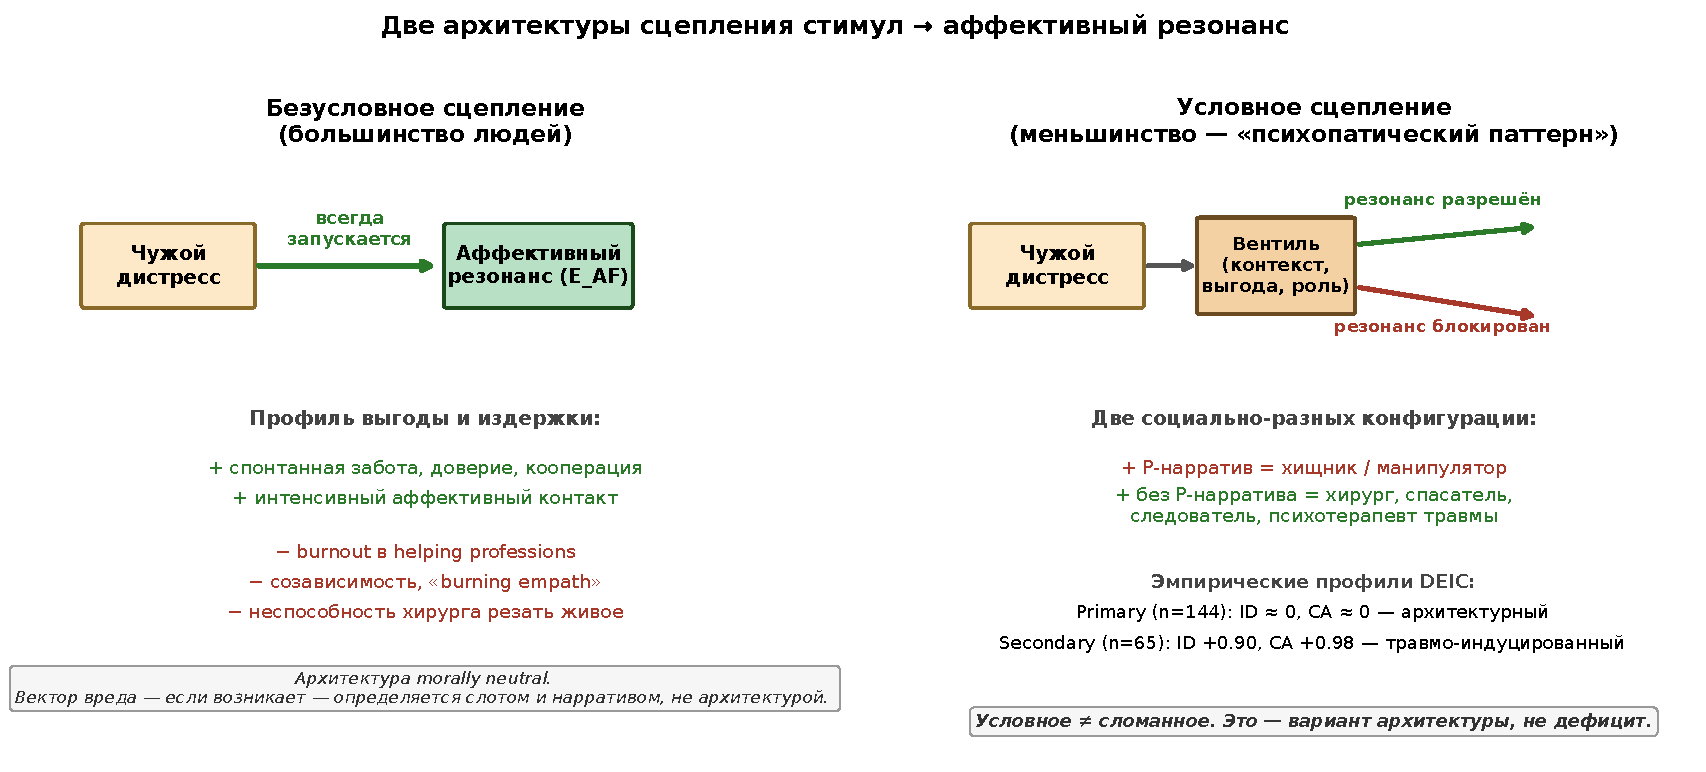
\includegraphics[width=0.95\linewidth]{figures/fig12_conditional_coupling.pdf}
\caption[Unconditional vs conditional affective coupling]{Architecture of \EAF{} coupling, not deficit. Left: \emph{unconditional} coupling --- affective resonance is triggered automatically, almost involuntarily, regardless of context and moral assessment (baseline pattern of the majority of the population). Right: \emph{conditional} coupling --- the same resonance is available but routed through a context-dependent gate; the combinations of this architecture with the P-narrative determine its social application. The empirical profiles of the primary ($n = 144$; ID $\approx 0$, CA $\approx 0$) and secondary ($n = 65$; ID $=+0.90$, CA $=+0.98$) cells are shown as two etiological trajectories into the conditional architecture.}
\label{fig:conditional_coupling}
\end{figure} Parallels in other functional systems help sustain the frame without a normative slide: people differ in the condition-sensitivity of the pain response, in autonomic reactivity, in the default level of arousal. None of these variations is labelled a malfunction by default --- each is evaluated in the concrete context of application.

Conditional coupling has an important double use that is usually crowded out of the clinical frame. In social roles that require working inside situations of suffering \emph{without} automatic affective entrainment, conditional architecture is not only compatible but functionally necessary. The surgeon who during an operation can stay cognitively precise while working with the living flesh and blood of a patient. The emergency physician who is effective in disaster precisely because affective resonance does not paralyse his actions. The investigator working with testimonies of sexual-violence victims. The trauma therapist sustaining many years of client states without burning out. Each of these roles requires \emph{conditional} access to affective resonance --- the capacity to turn resonance coupling on and off deliberately. Unconditional architecture in these roles yields high burnout vulnerability; conditional architecture gives stability. At population scale this variation serves functions that society otherwise could not fill.

This architecture becomes harmful only in combination with the \textbf{P-narrative} --- a stable moral claim ``this is permitted to me'' that turns conditional coupling toward deliberate instrumental use of others without moral obligation. This is precisely why \DEIC{} models P \emph{separately} from \EAF{}: the affective architecture in itself is morally neutral, and the moral narrative is an orthogonal layer that determines its social application. Conditional coupling without a P-narrative --- surgeon; conditional coupling with a P-narrative --- predator. Unconditional coupling with a P-narrative is an unlikely combination, rare in the data; unconditional coupling without a P-narrative is the baseline empathic pattern of most of the population, with its own vulnerabilities.

In our data this two-layer logic is visible in three empirical results. First --- \textbf{parallel mediation CA $\to$ \{ID, P, M\} $\to$ \EAF{}} in a unified model (§\ref{sec:results}.4.1): the CA $\to$ P path is essentially empty ($a$-coefficient $+0.015$, indirect effect 95\% CI $[-0.086, +0.060]$ includes zero), while the path via ID carries $\sim 173\%$ of the total CA effect on \EAF{}. At the population level P and CA are statistically orthogonal. This means the P-narrative is \emph{not} an adaptive consequence of childhood history but an architecturally independent layer. The secondary (hi-P-hi-CA) pattern is not ``P via CA'' but the co-occurrence of two independent axes in a subgroup of people. The primary (hi-P-lo-CA) pattern accordingly is not ``psychopathy without childhood trauma''; it does not belong to the same etiological line as the CA-mediated constructs at all.

The parallel-mediation result requires honest reconciliation with the unified SEM (§\ref{sec:results}.4.2), in which all paths --- parallel mediators, A main-effect on \EAF{}, and A moderation of both stages of the ID channel --- are estimated simultaneously. In that fuller specification the $a$-path CA$\to$ID remains robust ($+0.345$), CA$\to$P is still empty ($+0.011$, NS), but the $b$-path ID$\to$\EAF{} collapses to $-0.012$ (NS) once P is included in the same equation, while P$\to$\EAF{} dominates at $-0.726$. The moderation index \IMM{}, significant in the narrower specification of §\ref{sec:results}.4 ($-0.00197$, CI not including zero), also collapses to $+0.0001$ (NS) when P and A are present as predictors of \EAF{} in the same model. This is not a refutation of §\ref{sec:results}.4 and not an artefact of overfitting --- it is a re-composition of variance. At population scale the main explanatory weight on \EAF{} concentrates in the P channel (the ``permitted to me'' narrative) and in A main-effect (witnessing as an independent positive predictor of \EAF{}, $b = +0.393$), not in an isolated ID$\times$A moderation. At the clinical case level the cascade CA $\to$ ID $\to$ reduced \EAF{} remains substantively meaningful --- the $a$-path is real, ID as a mediator of traumatic experience in individual dynamics is present; but when we look at the whole sample, the direct negative predictor of affective empathy is not residual ID but the active P-narrative and (on the other side) active witnessing presence.

This refinement is important because it changes the clinico-theoretical formulation without losing the main content. We do not claim that the ID channel is absent. We claim: at the level of the whole population, the ID channel and the P channel share a substantial amount of variance in predicting \EAF{}, and in the unified model P carries the main weight (with its moral signature) alongside A (with its witnessing layer). This result strengthens rather than weakens the thesis of §\ref{subsec:architecture} about two-layer architecture: the architectural level (conditional/unconditional coupling) and the narrative level (P-permission) operate \emph{independently} of childhood history --- and their combination determines the social application of empathy far more strongly than residual ID dissonance on its own. ID is an important indicator of \emph{what is happening} inside a traumatized psyche; P is the decisive predictor of \emph{what this architecture unfolds into} at behavioral output.

Second --- separation of the primary and secondary patterns. Through a rule-based $2\times 2$ topological classification we identify the \textbf{primary pattern} ($n = 144$): conditional coupling without a traumatic history, with a pronounced P-narrative, without internal conflict (ID $\approx 0$, CA $\approx 0$). This is a configuration stable over time, not requiring a traumatic source --- an architectural variation onto which the P-narrative is ``superimposed'' as an independent moral structure \citep[in the terms of][empirically --- in similar proportions in \citealp{lilienfeld1990, patrick2010}]{karpman1941}. \textbf{Secondary pattern} ($n = 65$): conditional coupling with a traumatic history (CA $= +0.98$), with active internal conflict (ID $= +0.90$), with high Masking ($+0.63$). This is a configuration in which the conditional coupling mode is functionally \emph{forced} by the defensive system: automatic affective entrainment would be destructive, and the psyche has built conditional coupling as an adaptation. The P-narrative here usually remains active, but is structurally different --- it protects the remaining self rather than opening access to predation.

Third --- the distribution of A (attention) across groups and its interaction with architecture. The primary pattern has moderate A without special correlations with ID. The secondary pattern has low A ($-0.55$) --- its conditional coupling operates \emph{without} a witnessing relation, which makes it painful for the carrier. This points directly to different clinical entry points: the primary pattern has no ``wound'' that can be healed, and working with it is structural-social and narrative (restricting the P-narrative through external frames, where appropriate); the secondary pattern has a ``wound'' in the form of preserved ID, and A-work shifts conditional coupling into the integrated mode --- the same profile as the integrated survivor of §\ref{subsec:integrated_survivor}, but arrived at from a different history.

This is not a reproduction of the \emph{taxon} of \citet{hare2003} and not a claim that primary and secondary are different biological species. We claim more modestly: the architecture of conditional coupling exists in the population as a stable variation, etiologically it is reached by at least two paths (without trauma --- primary; via trauma as adaptation --- secondary), and the clinical interpretation ``psychopathy'' conflates these paths because at the behavioral level they look similar. They can be distinguished only through measurement of ID and CA. Without this distinction, therapeutic strategies systematically err: trauma-oriented interventions for the primary pattern land in emptiness; behavioral restrictive interventions for the secondary pattern ignore its internal conflict and potential resource.

The size of the secondary subgroup ($n = 65$) does not permit reliable effect-size estimates; this limitation requires a clinical sample for confirmation. But the direction of the distinction reproduces robustly in the latent topology and is not an artefact of any single index.

This reformulation --- architecture instead of deficit --- has consequences beyond the clinic. In the criminal-legal system, where psychopathy is often treated as a combination of moral and functional malfunction, separating architecture (neutral) from the P-narrative (morally significant) distinguishes what requires correction from what is not in principle subject to correction (architecture). In organizational psychology, the separation allows one to see that some roles require conditional architecture and that its ``treatment'' runs against function. In public communication, it allows one to stop speaking of psychopaths as ``broken people'' and move to a conversation about a combination of capacities and narratives that society can regulate through external structures, rather than through attempts to remake the inner architecture.

\subsection{Positioning: elephant, not master-map}
\label{subsec:positioning}

We deliberately choose a positioning that differs from most integrative psychological projects. \DEIC{} does not claim to be ``the first unified framework of empathy'', ``the resolution of the dispute between psychoanalysis and neuroscience'', ``the integration of all traditions''. We choose a narrower and more defensible position: \DEIC{} is a \emph{compression}, not a \emph{summation}. Different traditions (psychoanalytic, attachment theory, cognitive neuroscience of empathy, mirror-neuron literature, clinical tradition of psychopathy from Cleckley to Hare, contemplative traditions of witnessing) really do touch the same subject in different ways, and each touch is real. Our contribution is that we measured six distinguishable functions in \emph{one} sample, showed their stable structural relations, and thereby made visible the \emph{joints} between what these traditions describe separately.

We deliberately do not take the position that \citet{wilber1995, wilber2000} took toward the traditions. Wilber asserted that there exists a \emph{super-map} (AQAL: four quadrants $\times$ levels $\times$ lines $\times$ states $\times$ types), on which every tradition occupies its hierarchically determined place. This is an ontological claim: the map is primary, the traditions secondary, and each sees only a fragment of the whole that the meta-theorist sees. In our work four real differences from this position are important and will be maintained as discipline, not stylistics.

First, level of claim. Wilber constructs an ontology --- a meta-metaphysical claim about how reality is organized. \DEIC{} constructs a measurement model --- a psychometric model of six functions on a concrete sample. The first is irrefutable by construction; the second must reproduce in new samples, and if it does not reproduce, it is refuted.

Second, hierarchy of coordinates. In AQAL levels are hierarchical and normative: integral $>$ pluralistic $>$ rational $>$ mythic $>$ magical $>$ archaic. In \DEIC{} the six coordinates are non-hierarchical. There is no preset position that ``high A is better'' or ``low P is better''; there are empirical correlations with outcomes, but these are consequences of data, not normative judgments. The ``integrated survivor'' is one profile among many, not a summit.

Third, relation to traditions. Wilber assimilates: each tradition gets a place on \emph{his} map, and its internal structure is reinterpreted through AQAL. \DEIC{} does not place traditions. We say: ``the construct X we measured correlates with what tradition A calls \textit{sākṣī}, what tradition B calls \textit{rigpa}, what tradition C calls self-remembering''. These descriptions within their own systems are autonomous. We do not embed the systems into \DEIC{}; we show where a psychometric coordinate of \emph{our} model correlates with what they describe.

Fourth, modesty about the not-understood. Wilber explains everything, including internal contradictions --- they are assimilated as ``a lower level looking at a higher one''. \DEIC{} has an explicit list of what it does not explain (see §\ref{sec:limitations}, §\ref{sec:future}): temporal scaffolding, mechanism of switching between ID and P, mechanism of the therapeutic force of A, individual differences in A-trainability, developmental branching in the $2\times 2$, evolutionary-ecological substrate, reflexivity of the observer. This is not a defect --- it is a boundary.

A short formula that will recur several times in this section: Wilber --- ``I see the whole; the traditions see parts of my map; you are now at level X''; \DEIC{} --- ``I see six measurable functions. Some traditions describe one of them more deeply than we do. The coordinate scaffolding is not metaphysics but statistics; it can and should be refuted.''

\subsection{The anti-Wilber discipline: hygiene of language}
\label{subsec:discipline}

The position of §\ref{subsec:positioning} is enacted through a set of disciplinary rules that must be satisfied in every paragraph. First rule --- every claim about a construct is accompanied by a falsifier. If we write ``A moderates the CA$\to$ID$\to$\EAF{} channel'', we are obliged to add: ``if in pre-registered replication the \IMM{} 95\% CI includes zero, this claim is refuted''. By this we distinguish \DEIC{} from systems that explain everything (and thereby explain nothing).

Second --- ban on hierarchy between factors. We do not write ``A is maturity'', ``integrated survivor is the highest point'', ``witnessing is a more developed level''. We write ``empirically linked to [concrete result]''. This may seem pedantic, but it is precisely at this point that most meta-theoretical projects slip off the rails: normative language is embedded invisibly and closes the path to empirical verification.

Third --- do not assimilate the traditions, but do not keep them at a symbolic distance either. We do not write ``Zen is about A''. We write ``Zen describes a similar construct in its system; its correlation with our model is such and such''. If we cannot make the second part of the statement, we do not make the first. At the same time we \emph{do} make the second part --- and we make it at length, when a tradition supplies an operational distinction that the psychometric literature has not yet reproduced. Cultural references (advaita, dzogchen, Fourth Way, contemporary non-dual, McKenna) in \DEIC{} are not decorative ornament and not a display of academic boldness at the expense of rigor; they are sources of hypotheses that we either formulate as falsifiable or omit without mention. The Bayesian prior on divergence between our data and a contemplative tradition is ``we have not yet measured what they distinguish'', not ``they were wrong''.

Fourth --- measurement model $\neq$ ontological claims. We do not write ``\DEIC{} describes the psyche''. We write ``\DEIC{} is a psychometric model of six functions on an $N = 1426$ Russian-language online sample''. This restriction of the claim protects us from turning into a meta-theory.

Fifth --- lexical discipline. \emph{Extends, operationalizes, is consistent with, replicates within our framework, provides psychometric coordinates for} --- allowed. \emph{Unifies, completes, first to integrate, resolves, supersedes, subsumes} --- forbidden. The choice of verb in a key claim of the program is the choice between serious work and meta-theoretical pretentiousness.

Sixth --- an obligatory ``what \DEIC{} does not explain'' section of visible size, not in a footnote (see §\ref{sec:limitations}--\ref{sec:future}).

Seventh --- reflexivity clause: the methodological paper of the program will contain an explicit section on the fact that the observer (researcher) with her own level of A affects what she is capable of measuring in the observed. This is a structural epistemological acknowledgment, not a mystical remark.

\subsection{Falsifiability as a structural level}
\label{subsec:falsifiers}

The generative character of the model is more important than its descriptive character. All predictions formulated in the previous subsections of the Discussion --- two-stage A-moderation of the CA$\to$ID$\to$\EAF{} channel, collapse of the $b$-path ID$\to$\EAF{} in the unified SEM, CA$\perp$P orthogonality at the population level, distinguishability of primary and secondary psychopathy, the \EAF{} effect in the integrated-survivor cell, hyper-instrumentation P$\to$\Ecog{}, and others --- are moved to a separate structural section (§\ref{sec:falsification}) in the form of claim/falsifier pairs with explicitly stated test requirements and consequences of refutation. That section is not an extended commentary on the Discussion; it states \emph{at exactly which observations} the claims of this paper should be considered false. For reading the Discussion this means: all claims in the findings register (``the data show'', ``the model yields'') have scientific status exactly to the extent to which §\ref{sec:falsification} formulates their falsifier. That section is not an appendix to the paper but the condition on which the paper belongs to the empirical genre rather than the rhetorical one.

\subsection{Relation to existing theories}
\label{subsec:relation_to_theories}

\DEIC{} is compatible with most of the main lines of research on empathy and psychopathy, but diverges from dominant interpretations at a number of points. We do not claim these lines are wrong wholesale; we point to places where our model departs from them.

\citet{baroncohen2011} --- EQ as a dispositional trait: in our model \EAF{} is a state regulated by A; the trait model misses the core of the mechanism. ``Psychopaths lack cognitive empathy'' --- a popular oversimplification; our partial correlations show the opposite: $r$(P, \Ecog{}) $= +0.32$ after partialling. Cognitive empathy in psychopaths is often \emph{elevated}; it is precisely this that makes ``predation'' possible, as described by \citet{blair2013} and \citet{baroncohen2011} under the heading of hyper-instrumentation. Hare's taxon-view of psychopathy --- we find no categorical kinds in our data. A dimensional model with two orthogonal etiologies describes the topology of our results more accurately. \citet{newman2003} response-modulation theory as a universal explanation of psychopathy --- in our P patterns cognitive attention is intact; the witnessing-affective coupling operates in a \emph{conditional}, not an unconditional, mode. Response-modulation captures part of this mechanism --- selectivity of attention --- but does not separate the architectural layer (conditional coupling, morally neutral) from the narrative layer (P-permission).

Classic attachment determinism \citep{bowlby1969} in its simplified reading: CA $\to$ dysfunction linearly. Our data show moderation through A. Determinism is false; compensation is empirically real. \citet{vaillant1977} hierarchy of mature vs immature defenses --- we do not find that defenses per se are pathological. ID without A yields dysfunction; ID with A --- functional compensation. The moral frame ``mature defense better than immature'' turns out to be less informative than the frame ``defense plus witnessing''.

NICE/APA CBT-first for all mood disorders \citep{nice2022, apa2019}. \DEIC{} directly predicts that in high-ID / low-A clients CBT lands in resistance or yields superficial improvement without change in the underlying mechanism. Self-reported psychiatric dx count as a severity measure --- our data show that ID blocks help-seeking, so dx\_count \emph{underestimates} the heaviest cases. FFMQ \citep{baer2006} as an operationalization of mindfulness --- our A-CFA empirically demonstrates that metacognitive items conflate attention-to-internal-states with witnessing. We support the critique of \citet{vandam2018}. \citet{wilber1995, wilber2000} AQAL --- we do not reproduce hierarchical-stage models of the development of consciousness in our data. We do not find stages; we find distributed non-hierarchical coordinates.

\subsection{ACE extension: ``don't remember'' as part of the construct, not as missingness}
\label{subsec:ace_extension}

The standard operationalization of adverse childhood experiences, descending from \citet{felitti1998} and established in the CDC/Kaiser line and in virtually all of the derivative corpus, admits two legitimate responses per ACE item from the respondent: ``yes'' (the event occurred) and ``no'' (it did not); everything else---``I don't remember,'' ``I am not sure,'' a refusal---is treated as missing data, excluded, or imputed. ACE items meanwhile ask not about emotional interpretation of childhood but about \emph{facts}: whether a parent was incarcerated, whether substances were used in the family, whether domestic violence occurred, whether a parent died, whether the parents divorced. To a factual question, ``I don't remember'' has, at the population level, exactly two substantive interpretations, and \emph{neither of them reduces to statistical missingness}. First: the respondent was not told---which is itself a marker of a family pattern of silencing around a high-adversity environment (families that systematically discuss a deceased parent or an episode of violence produce different respondents than those that answer ``don't remember''). Second: the respondent dissociated---which is a direct behavioral manifestation of the very defensive mechanism D that the ID latent measures at the other end of the instrument. Both interpretations are ACE-relevant; both are empirically opposite to treating ``don't remember'' as missing. The standard coding in that case \emph{excludes from analysis precisely the sub-contingent in which the ACE signal should be strongest}. This is not a minor coding detail but a structural undercount in the standard ACE methodology, inherited by the whole corpus.

The DEIC construct proposes an extension: ``don't remember'' on an ACE item should be treated as a \emph{positive signal of an adversity-relevant family or cognitive configuration}---either of family silencing or of a dissociative encoding gap---and coded numerically on par with ``yes.'' ACE then ceases to be a one-dimensional event counter and becomes two-layered: an explicit count of confirmed events plus a count of ``don't remember'' responses as a separate ACE-dissociation subscale.

Empirical validation of the extension was obtained on the present sample through a full re-fit of the 6-factor oblique CFA in which the canonical code ``don't remember''~$=$~NaN was replaced with ``don't remember''~$=$~1. Of 1470 respondents, 667 (45.4\,\%) used ``don't remember'' at least once across the 10 ACE items; 294 (20\,\%) used it twice or more. Under the extended coding, N passing the $\le 10\,\%$ missing filter rises to 1468 (vs. the canonical 1426); mean ACE count shifts from 3.43 to 4.18; MLR-robust CFA retains acceptable fit (CFI~$=$~0.960, TLI~$=$~0.949, RMSEA~$=$~0.062 against canonical 0.950, 0.936, 0.068; df~$=$~120 in both cases). Latent correlations in the 6-factor oblique model shift in the direction consistent with the DEIC hypothesis: $r(\text{CA}, \text{ID})$ rises from $+0.668$ to $+0.712$; $r(\text{CA}, \EAF{})$ strengthens in magnitude from $-0.129$ to $-0.205$ ($+59\,\%$); $r(\text{CA}, M)$ rises from $+0.195$ to $+0.267$; while $r(\text{CA}, P)$ remains weak (rising from $+0.015$ to $+0.122$---still within the ``weak'' range), preserving the architectural orthogonality of P to childhood adversity.

Parallel mediation CA~$\to\{$ID, $P$, $M\}\to\EAF{}$ on latent scores in split-B, under canonical and extended coding with 5{,}000 bootstrap draws, yields a consistently strengthened picture. The total effect $c$(CA~$\to$~\EAF{}) strengthens in magnitude from $-0.129$ to $-0.205$. The indirect effect through ID---the canonical ``defense kills empathy'' channel---retains its structure: $-0.223$ [$-0.267, -0.181$] under canonical coding, $-0.236$ [$-0.282, -0.192$] under extended; the CI excludes zero in both cases. The indirect effect through P \emph{becomes statistically distinguishable from zero} precisely under the extension: canonical $-0.014$ [$-0.086, +0.060$] (NS), extended $-0.140$ [$-0.234, -0.048$] (statistically significant). This does not redefine the architectural orthogonality of P to CA as a population fact, but it indicates that part of the P channel had been instrumentally under-detected precisely where respondents had engaged dissociative encoding of childhood. The direct effect $c'$ (CA~$\to$~\EAF{} controlling for ID, P, M) remains positive under both codings ($+0.073$ canonical, $+0.048$ extended); that is, the headline sign flip of the principal mediation conclusion---``trauma damages empathy via the defense, not directly''---is robust to the coding of ``don't remember.'' No 95\,\% bootstrap interval of the originally significant indirect effects crosses zero under the extended coding; the shifts are numerically detectable rather than noise.

The operational implication for wave 2: ACE items retain a three-option format ``yes / no / don't remember,'' but ``don't remember'' is coded as a positive signal; the counter of such responses across all 10 items is constructed as an independent ACE-dissociation subscale. Psychometric prediction: at $n \ge 300$, this subscale should yield McDonald's $\omega \ge 0.7$ and correlate positively with the ID latent ($r \ge 0.30$ at the latent level); when it is controlled, the association of the ``explicit'' ACE count with ID should attenuate, which provides a formal test of the subscale's validity as a distinct channel. The conceptual implication is broader. We do not claim a generalization of \emph{effect sizes} to the entire ACE literature---that would require a meta-analytic re-fit; we point to a \emph{structural} problem in the coding logic inherited by the whole corpus \citep{felitti1998}. Wherever that logic is identical, the directional meaning-constructing shift is identical: any self-report of sensitive information from early life---sexual history, substance history, family secrets---in which ``don't remember'' is a legitimate and socially acceptable response, requires explicit modeling of that response as a construct-relevant signal, rather than mechanical reduction to missing. See §\ref{sec:future} for the wave-2 design and §\ref{sec:limitations} for the boundaries of the present estimate.

\subsection{Declarative--behavioral asymmetry (DI) as a signal of architectural fragmentation}
\label{subsec:di_asymmetry}

The pilot composite version of the instrument (DEIC-DRAFT, August 2025) was built on the principle of paired formulations: each content item existed in a declarative register (abstract self-description: ``I am an empathic person,'' ``I manipulate others,'' ``I suppress my emotions'') and a behavioral register (a concrete narrow-window behavioral report: ``yesterday I stopped and really listened,'' ``last week I hid an important detail from my partner for my benefit,'' ``this morning I refrained from showing irritation''). The summary index $DI = \overline{\text{decl}} - \overline{\text{beh}}$ across all items in the pilot showed a statistically significant population shift ($p < 0.001$, $d \approx 0.43$), with the leading contribution from the AIS scale (declarative 5.04 vs. behavioral 3.35). On this basis DI was described in the pilot report as an independent indicator of social desirability. Below we show that this description was partially wrong: the population shift replicates, but across scales it is bidirectional, and what DI actually measures is not a uniform self-presentation distortion but an \emph{architectural gap between abstract self-schema and episodic behavioral recall}.

On the main sample ($N{=}1470$) the declarative--behavioral gap was computed across eight scales with sufficient paired-item balance (ADI, CA, D, EC, Empathy, Psychopathy, Suppression, Masking; 38 declarative against 40 behavioral). Paired $t$-tests are significant on all eight scales, but the distribution of $d$ in magnitude and direction differs substantially. Positive DI (declaration exceeds behavior)---E ($d{=}{+}0.44$), EC ($d{=}{+}0.45$), ADI ($d{=}{+}0.20$), CA ($d{=}{+}0.19$). Negative DI (behavior exceeds declaration)---P ($d{=}{-}1.05$; the largest effect on the sample), MS ($d{=}{-}0.30$), S ($d{=}{-}0.10$), D ($d{=}{-}0.09$). The summed raw DI turns out to be weakly negative ($d{=}{-}0.11$)---the sign of averaging oppositely directed scales. If DI is aligned in the prosocial direction (for stigmatized scales the sign is reversed, so that $+$ always means ``I pass declaratively as a more positive version of myself than my behavior shows''), the shift becomes uniformly positive: $d_{aligned}{=}{+}0.29$, 95\,\% CI $[{+}0.14, {+}0.20]$. The pilot observation therefore replicates, but as a \emph{joint outcome of two different mechanisms} rather than as a uniform social-desirability bias.

Disentangling these mechanisms is the principal substantive result of this subsection. For stigmatized scales with explicit self-incriminating content (P, MS, S, D), narrow-focus behavioral items (``this week I \ldots'') collect more admissions than declarative trait descriptions---what the respondent is unwilling to own as a trait, they are willing to acknowledge as an episode. This is most vivid on P: the pair $P_4$ (``I manipulate people to get what I want'') vs.\ $P_{\text{new\_3}}$ (a concrete behavioral description of an exploitative situation within the preceding period) yields a mean gap of $-2.66$ points on a 7-point scale ($d{=}{-}0.98$); that is, the respondent systematically denies the trait schema of psychopathy but clearly recognizes concrete manifestations of it in their own behavioral archive. This reproduces at an operational level a long-standing clinical observation about the split between trait identification and episodic behavioral self-report under a psychopathic narrative \citep{hare2003, lilienfeld1990}. For desirably valenced scales (E and, with a qualification, EC), the direction is opposite: the trait schema is broad, the behavioral episode is narrow---the respondent holds a developed self-presentation as empathic, supported by a wide history, while a concrete narrow-window behavioral item (``this morning I \ldots'') does or does not land in a specific behavioral episode. For shared-adversity scales (ADI, CA) a positive gap points to the opposite pattern: the trait level partially overstates an inner history that the concrete behavioral episode in ordinary life does not confirm---a possible methodological consequence of ADI- and CA-declarative items querying a global affective self-concept not tied to recent code.

That DI does not reduce to social desirability is confirmed by its connections with the latent architecture. $DI_{overall}$ (raw, undirected) correlates with ID as $r{=}{+}0.590$, with CA as $r{=}{+}0.580$, and with A as $r{=}{-}0.517$; with the clinical diagnostic variable ($\text{dx\_free\_text\_any}$)---$r{=}{+}0.017$ (NS, $p{=}0.66$). In other words, the magnitude of the declarative--behavioral gap tracks the \emph{internal fragmentation between the trait-self-schema layer and the episodic-behavior-recall layer}, and this fragmentation is marked by the same architectural latent (ID) that elsewhere in the work is registered as the defensive contour. $A$ as a witnessing function narrows the gap. Clinical status plays no role here, which is structurally consistent with §\ref{subsec:architecture} and §\ref{subsec:free_will}: DI is an architectural, not a diagnostic, metric. $DI_{aligned}$ (rotated in the prosocial direction) gives a mirror image: $r(DI_{aligned}, A){=}{+}0.658$, $r(DI_{aligned}, \EAF{}){=}{+}0.550$, $r(DI_{aligned}, ID){=}{-}0.645$, $r(DI_{aligned}, P){=}{-}0.362$. Under a median split on $A$, the contrast of $DI_{overall}$ between low-A and high-A yields $d{=}0.90$ (tertile contrast $d{=}1.22$); the $A$-field fully restructures the direction and magnitude of the gap.

A separate finding concerns $piz$---the integral metric implemented in the instrument for tracking facade work (masking + lie; §\ref{subsec:integral_metrics}). $piz$ and DI are structurally and empirically distinct. $r(piz, DI_{overall}){=}{+}0.198$ (small positive), $r(piz, DI_{aligned}){=}{-}0.274$---that is, $piz$ and $DI_{aligned}$ diverge even in sign (higher masking $\Rightarrow$ \emph{smaller}, not larger, prosocial shift of declaration over behavior). On individual scales $r(piz, DI_{P\_scale}){=}{+}0.359$: higher masking is associated with a more pronounced $\textit{beh}>\textit{decl}$ gap on the P scale (high facade work amplifies precisely the asymmetry in which trait denial goes hand in hand with behavioral acknowledgment). In sum: $piz$ measures self-presentational pressure, $DI$ measures structural fragmentation---two distinct layers, both operationalizable.

For instrument infrastructure this means that $DI$ should be recorded alongside $piz$ as a sixth \texttt{extended\_metric} in \texttt{psychometrics.json} (with per-scale and overall-aligned versions). For the theoretical frame it means that the pilot observation is recovered, but in a substantively refined status: it supplies an operational psychometric grid for the long-standing psychoanalytic distinction between the ``ideal self'' as trait-schema and the ``acting self'' as behavioral archive \citep{freud1917, winnicott1965}, where the gap between them is not a measurement defect but a substantive marker of architecture. The methodological implication for wave 2: any psychometric scale claiming a diagnostic function in the $ID$/$P$/$E$ domains must include paired declarative and behavioral formulations, because it is their gap, rather than either formulation in isolation, that provides access to the architectural layer.

\subsection{\DEIC{} and the theory of consciousness: the boundary at which we work}
\label{subsec:consciousness}

\DEIC{} does not offer a theory of consciousness. The hard problem \citep{chalmers1995} is a boundary that psychometrics does not cross and must not pretend to have crossed. We measure functions \emph{within} consciousness (attention, dissonance, empathy); we claim nothing about the nature of subjective experience as such, and this restriction is serious, not rhetorical.

But from the reality of the boundary it does not follow that one should keep distant from it. On the contrary: it is precisely near this boundary that the most substantive interface of empirical psychometrics with contemplative studies arises. A is the psychometric trace of what various traditions single out as a structurally different layer of consciousness: \textit{sākṣī} in advaita, \textit{rigpa} in dzogchen, ``self-remembering'' in Gurdjieff, non-dual awareness in the contemporary non-dual literature. We do not explain what the witness is. We show that witnessing is measurable, functional, and that its action on the CA$\to$ID$\to$\EAF{} channel reproduces in the narrow specification. This makes A the point at which psychometrics \emph{comes into contact} with the part of consciousness usually treated as non-functional --- without assimilating it and without claiming its nature, but without skirting it either.

The sharpest dialogue of this type is with \citet{mckenna2002, mckenna2004, mckenna2013}. In most Western representations of contemplative traditions, awakening is described additively: more awareness, more acceptance, more presence. McKenna inverts this. His thesis is \emph{spiritual autolysis}: awakening is a destructive process, the dissolution of illusory structures, not the accretion of new capacities. More attention does not bring consolation; it reveals the constructedness of one's own states and of the world, and this revelation is not pleasant. The ordinary person avoids it, because there is no consoling frame there.

In the \DEIC{} frame McKenna's thesis becomes a direct longitudinal prediction. In people going through intensive retreats with deep witnessing practice, A rises. If McKenna is right, over a short time-interval ID \emph{rises} --- the revelation of constructedness produces temporary destabilization of identity, which is precisely the signature that in our cross-sectional model we read as dissonance. The trajectory then branches: either regression (defenses return, A falls back, the destabilization closes through the usual structure), or integration (acceptance of constructedness, a profile topologically corresponding to the integrated survivor of §\ref{subsec:integrated_survivor}, but arrived at not through childhood trauma but through a voluntary practical path). This is not a prediction of ``is McKenna right''; it is the operationalization of his thesis in a form that can be refuted by longitudinal data on retreat cohorts.

This is our position relative to the theory of consciousness. Not to replace it, not to claim its territory --- but not to make its existence an excuse to avoid contact either. Work at the boundary is possible and necessary: making concrete psychometric predictions at points where contemplative traditions hold operable distinctions that empirical psychology is only beginning to capture.

\subsection{Clinical implications}
\label{subsec:clinical}

The model has several concrete clinical implications, which we formulate as \emph{proposals for testing}, not as recommendations for immediate adoption.

\paragraph{Work with A before work with content.} In clients with high ID and low A a direct cognitive intervention often lands in resistance or yields superficial improvement. Our model predicts that the sequence ``A-work $\to$ content-work'' will be more effective than ``content-work without prior A''. This formalizes what somatic experiencing \citep{levine2015}, sensorimotor psychotherapy \citep{ogden2006}, IFS \citep{schwartz1995}, mentalization-based therapy \citep{fonagy2008}, and a range of psychodynamic approaches do intuitively. A pre-registered RCT with baseline A and ID as moderator of treatment effect is a direct test.

\paragraph{Distinguishing primary and secondary patterns in clinical assessment.} Without measuring ID and CA the two patterns look identical but require different strategies. Primary --- conditional architecture without a ``wound'': clinical work with the architecture as such is useless and may even be inappropriate (in functional social slots this architecture gives stability); work with the P-narrative through external frames is appropriate when the narrative turns predatory. Secondary --- work with trauma and expansion of A, aiming to shift the preserved ID into integrated mode.

\paragraph{A-training as the central component of long-term work.} Our model predicts that non-dual mindfulness practice will yield a stronger effect on \EAF{} recovery than behavioral mindfulness in the MBSR style. This formulates a head-to-head testable comparison.

\paragraph{Burning empath as feed-forward risk.} The profile CA + hi \EAF{} + lo A should predict burnout in helping professions.

\paragraph{Substance use as phenotype, not cause.} In the subgroup of blocked-sober-high-P the same P/D/ACE profile is observed as in active substance users. This indicates that substance use is an \emph{exit} from blocking, not its source. A-training in work with addictive behaviors should give a stable effect where abstinence-based programs relapse.

\paragraph{A therapist with low A does not see the client's ID activation.} This has a direct clinical consequence: supervision and self-work of the clinician are not a ``nice to have'' but a structural condition of the possibility of seeing what is happening in the client.

\subsection{Free will as a gradient of attention}
\label{subsec:free_will}

One of the most conceptually heavy consequences of \DEIC{} is a reformulation of the problem of free will. We do not claim to solve it. We claim that in its classical binary form --- ``is the will free?'' --- it is posed at the wrong grain and therefore has no answer. At the grain our model provides, it decomposes into a concrete empirical question: \emph{what is the magnitude of A in a given situation for a given agent?}

In \DEIC{} coordinates, behavior can be read as the result of interaction between two layers: the automatic D/P/E configuration (what triggers in response to a stimulus without participation of a witnessing relation) and A (the gap between trigger and action, in which a different distribution of attention, a different relating, a different reaction becomes possible). A low-A agent at a given moment is functionally determined by her configuration: the stimulus activates the channel, the channel unfolds automatic behavior, observation is absent. A high-A agent at the same moment has a \emph{measurable gap} between activation and action, within which a different trajectory is possible. This is not a metaphysical distinction but an empirical variable --- the same one our A-moderation fixes in the narrow specification: at high A the CA$\to$ID$\to$\EAF{} channel flips sign precisely because A wedges between the habitual trigger and its habitual outcome.

Philosophers who asked about free will approached the same gradient from different sides. Augustine's ``slave of the will'' and his description of \textit{liberum arbitrium captivatum} is a description of the low-A state, in which desire continuously unfolds into action without a gap. Kant and his primacy of practical reason --- a description of a function that appears at high A: the \emph{Maxime} as a conscious principle of conduct, not an impulse. \citet{libet1985} with his early readiness potential and the critics of his interpretation \citep[see][]{frith2008} point out that a voluntary act does sometimes lag behind brain activity, but the \emph{veto function} remains --- this is A, holding the gap. \citet{frankl1946} --- ``between stimulus and response there is a space; in that space our power lies to choose our response'' --- a direct description of A-moderation in clinical language. Buddhist \textit{vīmaṃsā} (investigative attention) and \textit{yoniso manasikāra} (wise attention) describe practices that build A as the condition of ethical possibility; the advaitic distinction between \textit{vṛtti} (movements of mind) and \textit{sākṣī} (the witness) --- the same structural asymmetry. Gurdjieff's ``man-machine'' is a description of the low-A mode, and ``self-remembering'' is an operational protocol for raising A. When these lines converge on the observation that the ordinary person acts out of automatism most of the time, and that moments of freedom are tied to a special quality of attention, they converge non-accidentally --- they describe the same measurable phenomenon in different languages.

From this reading a series of predictions follows. First, the agent's perception of his own voluntary act as ``free'' should correlate with his momentary A, not with his trait-level self-efficacy or with the narrative of self-determination. Paradigms of the \citet{westgate2019} meaning-in-action type can be reframed as A-assays. Second, interventions that raise A (non-dual mindfulness, somatic work, psychedelic integration) should produce measurable growth in variables usually associated with self-determination: intrinsic motivation, moral consistency, capacity to forego short-term reward for a long-term value. Third, populations with systematically suppressed A (see §\ref{subsec:political}) should display systematically reduced functional freedom of choice --- not as a moral defect but as a direct consequence of the destruction of the operational infrastructure of freedom.

The ethical consequence of this reading is not the abolition of responsibility but its structural recalibration. The question ``was he free in that moment?'' acquires an empirical answer: what was his A-configuration at the moment of action, what was the variance of his A over time, what is the trajectory of its development. Responsibility is preserved but distributed differently: for a concrete act at a low-A moment --- lower in intensity than for the long-term trajectory of care for one's own A infrastructure. This coincides with the intuition that clinical common sense and a number of legal systems already use de facto (mitigating circumstances, diminished capacity, forensic assessment of the state at the time of the act), but makes it operational. Forgiveness, which in most traditions is formulated ethically (``forgive them, for they know not what they do''), becomes an epistemologically correct attribution: at a low-A moment the agent did not know, because the infrastructure of knowing was not deployed.

We stress that this does not abolish the difference between acts produced out of low-A automatism and acts produced with A support from a pronounced P-narrative. The former are structurally unfree, and standard therapeutic and educational work is, as a rule, the adequate response. The latter are architecturally different: high A, holding the P-narrative ``this is permitted to me'', is not the absence of freedom, but a choice out of high A in favour of violation. The social and legal response to these two classes of acts must be structurally different, and \DEIC{} supplies a coordinate grid in which such a distinction can be made operationally, not impressionistically.

\subsection{Politics, media, attention: \DEIC{} at social scale}
\label{subsec:political}

The outputs of \DEIC{} beyond individual clinic require a separate discussion. We formulate them as \emph{theses for discussion for future research programs}, not as ready policy recommendations. The link between the architecture of individual psyche and social patterns is not direct, and every claim at the social scale on the basis of an $N = 1426$ Russian-language online sample is a hypothesis, not an established fact. But it is precisely because \DEIC{} contains explicit operational coordinates that these hypotheses can be formulated so that they can be tested.

\paragraph{Political demagoguery as a P$\times$low-A market.} A political style that the literature describes as populist/demagogic has, in \DEIC{} language, a clear signature on the leader's side: high P (the moral narrative of permission --- ``I lead them, I am allowed to decide for them''), moderate conditional \EAF{} (enough for ritual performance, not paralysing action), and --- \emph{crucially} --- high \Ecog{} (instrumental understanding of the audience). This is not an ad hominem attribution to concrete politicians --- it is a description of the structural niche which, in a population with low A, becomes socially adaptive and selectively preferred. \citet{westen2007, haidt2012} show that audiences vote not so much rationally as through moral and identificatory circuits; our framework sharpens this: audiences with low A-infrastructure choose not ideas but moral narratives that coincide with their own unreflective self-concept. Prediction: electoral support for P-style demagoguery should be predictable not by socioeconomic markers as such, but by the general A-level of the audience at the time of the election.

\paragraph{Attention economy as a structurally psychotogenic environment.} If A is the structural condition of integration and therefore the condition of the possibility of a stable psyche (see §\ref{subsec:integrated_survivor}), then an environment systematically destroying A acts as a psychotogenic agent at population level. Contemporary engagement-optimized media systems are structurally such an environment. The mechanism is three-layered: (a) fragmentation of A through micro-interruption (notifications, continuous feed, swipe interfaces), (b) surfacing of P-content as an engagement maximum (outrage, moral indignation, identity signaling), (c) delivery of consoling D-content (echo-chamber confirmation of the existing defensive configuration). In sum: simultaneous decline of A, growth of P-patterning in mass communication, stabilization of D. This is a reading of the observed ``epidemic of anxiety/ADHD/polarization'' not as an epidemic of separate disorders, but as a single structural degradation of the \DEIC{} configuration in the population. Concrete testable predictions: (i) intensity of use of engagement-optimized platforms predicts a decline in A in 6--12-month longitudinal studies; (ii) adolescent cohorts with early exposure to algorithmically-curated feeds have a measurably different \DEIC{} topology than cohorts with the same ACE load but without early exposure; (iii) experiments with attention-protective design (edit-mode, pause interfaces, slow-feed) should yield a measurable gain in A, other things equal.

\paragraph{Democracy as an A-dependent institution.} We formulate this cautiously, because a claim of this scale requires data of correspondent scale. Nonetheless: if democratic participation structurally presupposes the capacity to hold a complex moral and cognitive object (a political decision) long enough to deliberate on it --- that is, presupposes A --- then democracy in an environment of systematic A-destruction cannot sustain its own function. This is not an argument against democracy; it is an argument that democracy has historically rested on an attention-protective infrastructure (church, education in its older form, slow media, communal institutions) which secularization and commercialization have not replaced with an equivalent. The result is a regression of politics into populism, polarization, high susceptibility to P-style. The practical consequence: investments in attention-protective institutions --- educational reform, a contemplative component in general pedagogy, regulation of engagement-optimization as a public health issue --- are structurally necessary for sustaining democratic function. This thesis cannot be directly tested on our sample, but it follows logically from the A-moderation of individual functioning we have found.

\paragraph{Cults, authoritarian movements, sectarian politics.} The frame allows the dynamics of cults and authoritarian movements to be read in a single logic: the leader carries the dominant P-narrative of selectedness or exclusivity; followers bring D and low A --- a search for external structure that will dispense with the need for independent observation; the cult provides apparent integration through external structure instead of inner A-development. This reading makes the reintegration work with ex-cult members and ex-radicalized persons not simply cognitive deradicalization, but restoration of the A-infrastructure the movement suppressed. Empirically testable: \DEIC{} profiles of people leaving cultic/authoritarian movements should be characterized by low A and a D profile preserved in a frozen form; long-term therapeutic work should be accompanied by growth of A and the release of held D-content.

\paragraph{Collective D and transitional justice.} Post-genocide, post-totalitarian, post-colonial societies carry a collective analogue of individual D configuration: systemically suppressed, affectively unintegrated relation to their own historical reality, transmitted transgenerationally \citep{yehuda2015, meaney2001}. \citet{herman1992} in her formulation of complex trauma points to the collective layer; our framework makes measurable the assumption that transitional justice (truth commissions, memorial practices, public historical reckoning) works precisely as collective D-work --- and thus is effective where it opens space for affective integration, and ineffective where it is reduced to a procedural legal form. The Russian-language sample on which our model is validated carries an elevated baseline CA/ID densely connected with two twentieth-century wars, repressions, and the nineties; we hypothesize (and await cross-cultural replication) that this is not cultural noise of the sample but a measurable collective D configuration reflected in individual psyche.

\paragraph{Religions, secular substitution, collective A-infrastructure.} We describe this as a thesis for discussion, seeking to stay equally distant from religious apologetics and secular dismissal. Empirically: the major religious traditions historically contained three functional components systematically working with \DEIC{} configuration --- A-training (prayer, meditation, ritual examen), D-aperture (confession, collective lament, ritual mourning), P-restraint (commandments, examination of conscience). Secular contemporary substitutes (therapy, wellness industry, philosophy of practical life) try to reproduce part of these functions in individual voluntary form, but without institutional-level continuity and without collective infrastructure. Forecast: secular societies must \emph{rebuild} the equivalent of a collective \DEIC{}-calibration infrastructure or accept the epidemiological costs. This is not an argument for returning religion to its historical forms --- it is an argument that the function those forms performed did not vanish because the forms did.

\subsection{Evolutionary scale: integration as a biological requirement}
\label{subsec:evolutionary}

The broadest conclusion we are prepared to formulate --- so that the reader can see the scale at which \DEIC{} can work, even if it does not fit into one empirical paper --- concerns the phylogenetic roots of D and P. D and P as architectures are ancient, evolutionarily prepared. D is an extension of the freeze response (vertebrate immobilization under threat) into the emotional and social domain. P is a derivative of the dominance strategy in primate social hierarchy. Both mechanisms were adaptive in the environment for which they were built: episodic acute threat with rapid resolution (freeze), local hierarchical competition with clear rules (dominance). Both architectures now activate in contexts for which they were not built --- chronic economic pressure, continuous media monitoring, complex symbolic social ecology --- and thus shift from adaptation to chronic maladaptation. This is evolutionary mismatch in its structural-psychological variant \citep[in the spirit of][]{lieberman2013, sapolsky2017}.

From this frame follows one of the most serious consequences of \DEIC{}, which we are prepared to defend as a hypothesis-thesis for subsequent empirical programs. \emph{We are probably the first generation in the history of the species for which an integrated adult life is a biological requirement, not a luxury.} Evolution did not engineer a mechanism of adult integration, because until recent historical-demographic shifts most people died or were structurally embedded in clan/tribal/ritual community life before unresolved D/P could destroy an individual life; short life, ritual infrastructure, embedded forms of collective A (see §\ref{subsec:political}) did the work of integration in place of the individual. A contemporary eighty-year-old, living in a nuclear family, with forty years of productive labour, with exposure to chronic informational stimulation, with an atomized social network --- lives with a defensive apparatus designed for temporary use in an environment that demands continuous integration of what evolution did not prepare for integration at all.

The consequence, which we formulate as a thesis requiring testing by long-term population-level data: \emph{contemplative and therapeutic work is not an improvement of baseline function, but a \textbf{precondition of survivability} in our current biological and ecological coordinates}. In this sense mass demand for therapy, the growing demand for meditation and psychedelics, the population-level interest in somatic practices --- are not cultural fashion but a biological signal that the configuration of the nervous system, shaped for an environment of twenty thousand years ago, is insufficient for the environment in which it now lives and requires additional individual intervening work to function.

In its empirical part this thesis generates concrete predictions: (i) population-level indicators of A (boredom tolerance, capacity to hold a single object, distress tolerance) should fall monotonically with growth of urban engagement-density; (ii) the incidence of clinical D-dominant disorders should rise not in proportion to ACE per se but in proportion to the \emph{gap} between ACE load and accessibility of integration infrastructure; (iii) cohorts with structural access to integration infrastructure (long-term therapy, retreat culture, contemplative education) should show a measurably different mental-health trajectory on a 20--40-year longitudinal scale than demographically comparable cohorts without such access.

\subsection{Structural under-sizing of contemporary care}
\label{subsec:undersizing}

The clinically most serious consequence of the \DEIC{} framework, deserving separate discussion: the contemporary mental-healthcare system is \emph{structurally} not of the scale at which its task is declared. This claim is sharp, and we understand its sharpness. We formulate it as a thesis for discussion and will try to defend it empirically rather than rhetorically.

Classical trauma therapy in its contemporary medical format --- 20 sessions of CBT, SSRI support, structured psychoeducational modules --- is effective for post-formation adjustment disorder: for an adult psyche with a pre-trauma structure for which trauma is a break in continuity requiring processing. For \emph{personality-formative early D}, when D-configuration formed in the first 3--5 years of life and became the ground of subsequent development --- cognitive style, attachment pattern, desire architecture, identity --- such therapy is structurally under-sized.

The reason is concrete. For early formative D \emph{there is no pre-traumatic self as a referent of restoration}. The whole structure formed as adaptation to unsafety; restoration means not return to something that was destroyed, but reorganization of a structure built on a D foundation. In terms that will be recognizable to contemplative lines --- the Buddhist \textit{saṃsāra} in its ethical aspect, the hesychast ``stripping of the old man'', the Sufi \textit{fanā} --- this is a process of reassembly, not repair. Work of this scale does not fit into a protocol with a predictable number of sessions and a standardized outcome.

What we know about methods of adequate scale. Traditional forms: long monastic retreats (3-year-3-month in the Tibetan tradition, multi-year vipassana, hesychast ascetic labour, Sufi \textit{halva}) required institutional continuity that has almost vanished in contemporary secular societies. Contemporary clinical analogues: long-term intensive psychoanalysis (4--5 sessions per week over many years in Kernberg-style work), therapeutic communities in the Soteria tradition \citep{mosher1999} --- an almost lost institution; multi-year ayahuasca cycles in traditional contexts and their contemporary therapeutic translations \citep[see][in a ceremonial framework]{nielson2018}; ibogaine and 5-MeO-DMT assisted protocols with extended integration \citep[in Mexico/Netherlands, see the review by][]{brown2019}; long-term IFS/somatic work (many years of work with gradual restructuring without catastrophic collapse).

What is \emph{not} present in contemporary mental healthcare: a secular, insurance-covered, mass-available path of adequate scale for early formative D. This is not ``inefficacy'' --- it is structural mismatch of instrument to task. \DEIC{} makes this diagnosis operational through the measurement of baseline D + A + CA: the instrument enables \emph{pre-treatment} stratification of clients into those for whom symptom-management intervention is adequate (adjustment-level D without early formation) and those for whom interventions of structural level are required (formation-level D with high CA loading and low A infrastructure).

This is not a call to abandon symptom management --- it is needed and useful within its niche. It is a call to stop using a symptom-management instrument as universal standard of care for structurally different tasks. Clinical consequence: another argument in favour of baseline \DEIC{} profiling becoming a standard of stratification in research and, prospectively, in clinical practice. To a patient with early-formed D referred to a 20-session CBT we currently offer a palliative protocol sold under the name of definitive treatment; \DEIC{} stratification allows an honest statement: for this structure a different intervention is needed, one that either does not currently exist in accessible form, requires private resources, or is located outside the medical frame (long-term somatic work, psychedelic-assisted therapy in its developed form, long-term group/therapeutic community). Restructuring the system to this scale is a separate program, outside the scope of academic psychology but logically following from our data.

\subsection{Pharmacology, nosology, diagnosis: \DEIC{} as a reorganizing coordinate}
\label{subsec:pharmacology_nosology}

If \DEIC{} is a correct operational coordinate, several adjacent areas can be re-read under this coordinate. We do not complete this unfolding in the current paper; we show how it might look so that the reader can see the scale at which the frame works --- and at which it is yet to be tested.

\paragraph{Pharmacology as \DEIC{}-modification.} If each psychoactive class is characterized by which component of the D/P/A configuration it modifies and in which direction, then clinical outcomes should be predicted not by a diagnostic label but by a \DEIC{} profile at baseline. Working hypotheses for subsequent empirical programs: \textbf{SSRIs} reduce D-salience, they do not dissolve D-structure --- hence the characteristic profile ``functional but switched off'' on long-term use and additivity with therapy only when the therapy contains real A/D work. \textbf{Benzodiazepines} stabilize D through suppression of thaw signals --- long-term use prevents integration by holding the material that would otherwise mobilize it. \textbf{Antipsychotics} weaken both the P-narrative (via frontal modulation) and the extreme of D (via dopaminergic dampening) --- explaining their cross-diagnostic functionality and their price in the form of a general A-flatness. \textbf{Classical psychedelics} (psilocybin, LSD, DMT, mescaline) --- the only known class that directly dissolves D through DMN disorganization; a differential consequence we formulate as direct testable predictions: psilocybin-assisted therapy should yield a large effect on D-dominated profiles (depression, PTSD, entrenched dissociation) and small or reverse effect on P-dominated profiles (narcissistic pathology, antisociality), because the mystical experience without a D substrate may reactively validate the P-narrative. \textbf{MDMA} --- the unique configuration ``E-ceiling + D-dissolve + A-preserve'', structurally compatible with D-dominant PTSD; in a P-dominant structure efficacy should decrease, and this distinction should emerge in post-approval clinical data. \textbf{Ketamine} --- the paradox ``dissociation to dissolve dissociation'': a short window of high plasticity in which stuck D thaws given adequate integration infrastructure. \textbf{Stimulants} --- A-bandwidth without modification of D or P: in neurodevelopmental ADHD (low ACE) --- a pure gain; in trauma-origin ADHD (high ACE + D fragmentation of attention) --- a gain in productivity but not in wellbeing. \textbf{Opioids} --- the homecoming class for safety-deficit D: they return to the body a regulation the early environment did not provide, which explains the high correlation of opioid addiction with ACE+D baseline and makes naïve will-based approaches to opioid dependency structurally mistaken. Each of these predictions is a separate test program; together they pose the question of whether clinical psychopharmacology can be reorganized around \DEIC{} profiles as a stratifying variable rather than around DSM labels.

\paragraph{Trauma therapies decoded via a unified \DEIC{} mechanism.} EMDR works as a forced insertion of A into D-sealed memory through bilateral stimulation --- hence its strong effect on D-trauma and small effect on the P-narrative. Somatic experiencing \citep{levine2015} --- titrated D-thaw through direct access to freeze-release in the nervous system, bypassing cognitive access; it works precisely because D formed preverbally. IFS \citep{schwartz1995} --- externalization of parts and rapid A-upgrade through naming; works both on D profiles (parts holding freeze) and on P profiles (parts holding the permission narrative). CBT --- A via the cognitive layer; strong on the P-narrative, weak on D (one cannot challenge an inaccessible feeling). Long-term psychoanalysis --- slow A through narrative, with transference as a live channel of access to D-material. Group therapy --- a four-layer interaction: a distributed mirror for A-bootstrap, co-regulation of D across several bodies simultaneously, peer-confrontation of P, dissolution of shame through parallel stories \citep[see collected common-factors reviews in][]{wampold2015}. Psychedelic-assisted therapy in groups --- the theoretical maximum for number of simultaneously engaged integration mechanisms, corresponding to the empirically emergent shamanic-traditional format. This typology is not a claim about the relative superiority of one school over another, but a proposed coordinate grid on which different schools are seen as complementary, working with different components of one \DEIC{} configuration.

\paragraph{Nosological reorganization.} We formulate this part as the most discussable. DSM in its current form organizes disorders by phenotypic surface (symptoms); the \DEIC{} reading suggests that a large number of DSM co-morbidities are multiple expressions of a single channel configuration. MDD + GAD + PTSD + dissociative disorders in DSM are often one configuration ``hi ACE + hi D-dissociation + hi D-suppression + moderate A'' in \DEIC{}. Non-response and relapse are predicted not by diagnosis but by profile. This is compatible with trans-diagnostic movements (HiTOP, RDoC) but more parsimonious than each --- working with fewer axes. We formulate this as a future test program: will the \DEIC{} profile at baseline reproduce a greater percentage of variance of clinical response than a DSM label, in a large retrospective re-analysis? If yes --- the nosological reorganization acquires empirical support. If no --- the framework narrows to more restricted applications. This is a testable, falsifiable claim, not a meta-theoretical pretension.

\paragraph{Self-report-based nosology has a lower boundary of observability.} This is an important limitation for all clinico-epidemiological literature: D blocks help-seeking and smears self-report, so dx\_count and analogous counters of clinical load \emph{systematically underestimate the heaviest}. Almost all normative psychology is built on a semi-transparent population --- on those whose D is low enough that they filled out a form, came to assessment, or turned up in clinical registration. This is not a technical quibble about specific data; it is a structural property of the entire methodological infrastructure. The \DEIC{} framework makes this blind spot explicit: when we see in the population a profile with very high D and very low A, we predict that this part of the sample is densely populated by people who would not have appeared in the data had we not made special efforts. Methodological consequence for further work: active recruitment of the type usually recommended in community psychiatry is not an option for improving the sample but a structural condition of its validity.

\subsection{Wave-2 redesign: from diagnosis to a new instrument}
\label{subsec:wave2_design}

Most of the limitations of the present work are not fundamental defects of theory but signals of instrument redesign. In this subsection we collect the data showing structural problems of wave-1 scales into concrete proposals for wave-2 \DEIC{}-Inventory. Not at the level of individual items (that is the task of psychometric iteration with cognitive interviewing and pilot study) but at the level of architectural decisions: which scales remain, which are split, which are absorbed, which receive new design. These proposals are a contract between the present paper and the future wave-2 publication: the latter will be able to reference this section as the diagnostic grounding of its structure.

\paragraph{A: dedicated witnessing scale, separated from hypervigilance.} Wave 1 used A as a composite of metacognitive items. Tier-5 A-CFA (§\ref{subsec:A_as_field_condition} and §\ref{sec:limitations}) showed: on an attempted reflective factorization of the \emph{purest} 17-item pool the loadings are bipolar (8 positive, 9 negative), and latent A in SEM flips the signs of key coefficients. Diagnosis: the item pool does not separate \emph{witnessing} (non-reflective observation-of-observation in the non-dual tradition) from \emph{trauma hypervigilance} (painful hyper-alertness to internal states, structurally \emph{strengthening} defense rather than weakening it). Both yield a positive self-report on ``I notice my internal states'' --- operationally they are different. Wave-2 proposal: \textbf{(a)} \emph{two separate latents} --- Witnessing (W) and Hypervigilance (HV) --- with content explicitly separated by four linguistic traditions (\emph{satipaṭṭhāna}, \emph{sākṣī}, \emph{rigpa}, self-remembering); \textbf{(b)} key descriptor of witnessing --- ``observation without intervention, without reactivity, without desire to change the content''; key descriptor of HV --- ``constant scanning for danger, anxious monitoring''; \textbf{(c)} differential-validity check: W should correlate positively with distress tolerance and interoceptive accuracy; HV negatively with distress tolerance. The dedicated W-scale is priority number one in wave 2.

\paragraph{M: split instrumental and reactive masking.} Wave-1 M had $\omega = 0.546$ versus $> 0.89$ for the other five factors, and the latent correlation $r(M, P) = +0.82$ provides no clinically meaningful distinction. Diagnosis: the M scale confounds two phenomenologically distinct patterns --- instrumental masking (conscious management of the façade, close to P: ``how to look the way I need to'') and reactive masking (automatic social adjustment under threat, close to ID: ``how not to become noticeable''). Wave-2 proposal: \textbf{(a)} split into M\textsubscript{inst} and M\textsubscript{react}; \textbf{(b)} M\textsubscript{inst} should have a high correlation with P and a low one with ID; M\textsubscript{react} the opposite; \textbf{(c)} validation through item wording with explicit distinction of intention and automatism.

\paragraph{ID umbrella: keep the conceptual centre, restore SUP as a separate latent, refine DIS and AIS.} Bifactor analysis (§\ref{subsec:id_bifactor}) showed heterogeneity of absorption of the five wave-1 defenses by the general ID latent: IDS ($0.66$) and FLA ($0.86$) are almost fully described by general ID; DIS ($0.54$) and AIS ($0.53$) retain about half of subscale-specific variance; SUP --- only $31\%$. Wave-2 proposal: \textbf{(a)} \textbf{ID} remains as an umbrella latent (Internal Dissonance, heir of IDS), with IDS items and FLA items as clean indicators; \textbf{(b)} \textbf{SUP} is restored as a \emph{separate latent of suppression} --- ego-syntonic conscious inhibition, not part of passive blocking; SUP should positively predict executive control and negative-affect regulation in the short term, but \emph{not} predict trait-ID; \textbf{(c)} for DIS and AIS the items are reworked with content-forced differences: DIS items emphasize ego-dystonic automatism of splitting; AIS items --- ``the content is there, the feeling is cut off'' (the classical intellectualizer); after rework we expect a bifactor with a clean general-ID structure and separate clean DIS/AIS specific factors.

\paragraph{E\textsubscript{AF} and E\textsubscript{cog}: separation at item-level, not post-hoc.} The split of empathy into affective and cognitive was made in the present work post-hoc, in response to the P$\leftrightarrow$E paradox. Diagnosis: the wave-1 E scale conflated both components in the same items, which algebraically guaranteed confounding. Wave-2 proposal: \textbf{(a)} separate item-sets for E\textsubscript{AF} (emotional contagion, affective resonance, somatic markers of another's state) and E\textsubscript{cog} (perspective-taking, mentalizing, intention-reading) --- exactly one factor per item in the primary scale; \textbf{(b)} minimal content overlap between the two subscales; \textbf{(c)} pre-registered prediction: a bifactor with general E and two specific factors should yield ECV\textsubscript{global} $< 0.5$ (components separable), and P at latent level should yield $r(\text{P}, \text{E\textsubscript{cog}}) > 0$ and $r(\text{P}, \text{E\textsubscript{AF}}) < 0$.

\paragraph{P: expansion of content coverage and separation of the moral sub-scale.} Wave-1 P operated on a relatively narrow single-dimensional pool close to the Psychopathic Personality Inventory (Lilienfeld \& Andrews, 1996) and Dark Triad (Paulhus \& Williams, 2002). Diagnosis: the published findings (hyper-instrumentation, orthogonality to CA, primary/secondary topology) were obtained on a relatively narrow item pool; the primary/secondary branching predicted by theory is not supported by content-differentiated design; the moral component of P (``permitted to me'', which distinguishes architectural psychopathy from professional dissociation) is not separated from the architectural (switching resonance). Wave-2 proposal: \textbf{(a)} expand content coverage with items specific to primary (coldness, callousness, \emph{low}-anxiety variant of Karpman) and secondary (reactive aggression, high anxiety, trauma-linked); \textbf{(b)} a separate sub-scale \textbf{P\textsubscript{moral}} --- items about what the subject considers permissible \emph{for himself} (not about others): ``for me it's normal to lie if it works'', ``my emotional rules differ from the common ones''; \textbf{(c)} architectural P\textsubscript{arch} --- items about the capacity for conscious switching of resonance: ``I can turn sympathy on and off depending on who I am talking to''. Prediction: P\textsubscript{moral} and P\textsubscript{arch} should be distinguishable (latent $r \approx 0.4$--$0.6$), but both should yield a positive partial with E\textsubscript{cog}.

\paragraph{CA and ACE: keep as a single latent, add sub-scales of trauma type.} Wave-1 ACE and CA are interchangeable on our sample (latent $r > 0.8$), hence combined into a single CA latent. Diagnosis: combining does not lose the shared variance of early relational history but blurs the difference between types of adverse experience (physical abuse vs emotional deprivation vs attachment instability vs sexual trauma). Wave-2 proposal: keep a single CA latent as primary, but introduce four observable sub-indices (CA\textsubscript{phys}, CA\textsubscript{emot}, CA\textsubscript{attach}, CA\textsubscript{sex}) for descriptive distinction while preserving the single latent for SEM channels.

\paragraph{Lie scale: shift from covariate to active corrective metric.} Wave-1 Lie scale worked as a social-desirability covariate; in the present work it enters the correction formulas of integral metrics (§\ref{subsec:integral_metrics}). Diagnosis: the Lie scale is useful, but in wave 1 uses the traditional social-desirability item-set (close to Marlowe-Crowne and BIDR), which conflates impression management and self-deception. Wave-2 proposal: split into IM (impression management --- deliberate distortion for the external observer) and SD (self-deception --- unconscious distortion of self-perception); different diagnostic functions: high IM with low SD means responsible self-presentation, high SD --- active defense of the self-image, relevant to ID structure.

\paragraph{Architectural decisions.} Three changes in the scoring infrastructure for wave 2, following directly from the limitations of §\ref{sec:limitations}: \textbf{(1)} a two-level \texttt{questions.json} with \texttt{factor\_weights} (for CFA with explicitly written cross-loadings) and \texttt{primary\_scale} (for composite sum scoring, one item $=$ one composite) --- eliminates multi-scale inflation; \textbf{(2)} the default published model is bifactor (general ID plus specific factors) rather than pure oblique, so that the emerging structure reflects actual heterogeneity; \textbf{(3)} A is moved out of the 6-factor oblique into a separate formative block, with a subsequent reflective witnessing scale as a parallel reference point.

The transition from wave 1 to wave 2 is not a cosmetic rework of scales but a structural transplant. The present paper documents the diagnostic grounds for each change; the next paper of the program (wave-2 validation, pre-registered, on a new sample) will refer to this subsection as its design base.

\subsection{Integral metrics: proposed clinical indicators}
\label{subsec:integral_metrics}

The archival \DEIC-4 meta-model used four integral metrics --- R, DI, DHI plus an overall D-score --- as applied clinical indicators. In the present work we reformulate them as \emph{proposed} (not established) tools for clinical stratification, with an explicit indication that they require cross-validation on a clinical sample before being used in diagnostic practice.

\paragraph{Scope restriction.} Integral metrics are not an alternative to factor scores for scientific use. They are an applied layer: summary information on the respondent's profile, convenient for the clinician but deliberately less rich than the full vector of six factors plus A. We present them here because the structural-architectural frame of \DEIC{} has an operational output into the clinic, and the clinician needs a compact language. All formulas below are \emph{proposals}, not validated cutoffs.

\paragraph{R-metric (Resonance potential).} A proposed summary metric of empathic capacity with social-desirability correction:
\[
R = \text{E}_{\mathrm{AF}} + 0.5 \cdot \text{E}_{\mathrm{cog}} + 0.3 \cdot \text{A} - 0.3 \cdot \text{Lie}.
\]
Interpretation: high R $=$ preserved affective empathy, supported by the cognitive component and the witnessing function, corrected for impression management. Proposed clinical threshold interpretation: R $> 1.0$~$\sigma$ --- integrated profile; R $< -1.0$~$\sigma$ --- blocked profile; intermediate values require profile reading via ID/P.

\paragraph{DI-metric (Defense Intensity).} A summary indicator of passive-defensive intensity:
\[
\text{DI} = \text{ID} + 0.3 \cdot \text{M} - 0.4 \cdot \text{A}.
\]
High DI means an active ID cascade supported by masking, under insufficient witnessing for its moderation. Operational meaning: DI $> 1.5$~$\sigma$ --- a predictor of difficult therapeutic contact before A-work, since the ID structure actively blocks the empathic channel to the therapist.

\paragraph{DHI-metric (Defense Heterogeneity Index).} An indicator of the inhomogeneity of the defensive profile --- how evenly the ID variance is distributed across subscales (wave-1 IDS, SUP, DIS, AIS, FLA; or wave-2 analogues). Formally:
\[
\text{DHI} = 1 - \frac{\max_i \sigma_i^2}{\sum_i \sigma_i^2},
\]
where $\sigma_i^2$ is the standardized variance of the $i$-th subscale of the respondent relative to the sample. High DHI means passive blocking is distributed among several surface mechanisms (multifaceted defense); low DHI means one mechanism dominates. Clinical meaning: high DHI predicts a more complex therapeutic route (different defense types require different interventions); low DHI --- a narrow but intense defense with a clear entry point for work.

\paragraph{P-modified empathy metric.} A separate metric for cases suspected of a psychopathic pattern:
\[
\text{E}_{\mathrm{net}} = \text{E}_{\mathrm{AF}} - 0.4 \cdot \text{P} + 0.2 \cdot \text{A}.
\]
Idea: in hi-P respondents a high E\textsubscript{cog} with low E\textsubscript{AF} and without witnessing support gives a profile of \emph{instrumental empathy}; E\textsubscript{net} penalizes this pattern. In integrated respondents E\textsubscript{net} is close to pure E\textsubscript{AF}.

\paragraph{Proposal, not validation.} All four metrics --- R, DI, DHI, E\textsubscript{net} --- are formulated from the general architecture of \DEIC{} and from wave-1 formulas with minimal adaptation; they have \emph{not} passed competitive validation against existing clinical instruments (IRI, TSCC, TAS-20, PAS, SRP-4) on a clinical sample. They are suitable for research description of profiles, but not for formal diagnosis. Clinical deployment requires: \textbf{(a)} competitive validation on a clinical sample ($n \geq 300$ patients with formalized DSM/ICD diagnoses); \textbf{(b)} ROC analysis with explicit cutoffs for treatment-matching; \textbf{(c)} prospective testing of treatment response stratified by DI and R. The wave-2 program includes such a study as a separate clinical paper.

\subsection{Toward the research program}

The present paper is the central empirical work of the future \DEIC{} program. The program comprises 18 planned papers distributed across five layers: empirical (psychometric validations on new samples, longitudinal, cross-cultural, informant convergence), integrative (connection with attachment theory, with psychoanalysis, with neuroscience), philosophical (A ontology as field condition, \DEIC{} and the theory of consciousness, reflexivity, free will), applied (clinical implications, public frame, political communication, education, pharmacology as a \DEIC{} coordinate, structural under-sizing of care), and meta (methodological reflexivity, observer problem, anti-Wilber discipline). The ambition of the project is distributed across the program; the central paper is narrowly formulated and modest in tone precisely to protect the long-term work from premature stylistic criticism.

\paragraph{Fertility as evidence: branchability of the frame as an indirect signal of validity.} We are aware that in the previous subsections (§\ref{subsec:free_will}--\ref{subsec:pharmacology_nosology}) the six coordinates of \DEIC{} are unfolded onto themes that usually belong to different disciplines: clinical practice, political communication, evolutionary psychology, pharmacology, nosology, philosophy of free will. We do this not by accident, and we do not consider it ``too broad for a psychometric paper''. We claim the opposite: a good operational frame, \emph{by its very construction}, should explain different things through one mechanism, and branchability is not its freedom but its control. A poorly built frame behaves in one of two ways --- it either explains nothing (too narrow, does not transfer beyond its own training set) or explains everything equally (too broad, postmodern, without a signature of mechanism). \DEIC{} must instead produce \emph{specific differentiated} predictions in each domain of application: not ``everything is D'', but ``this phenomenon is D-dominant, that is P-dominant, that is A-deficit, and this is a combination with a specific topology''. If the frame sustains this differentiation across five different domains simultaneously, this is a weak but non-trivial inductive support for its validity. If in any of the domains it flattens to ``everything is explained by one coordinate'', this is a signal that the frame does not hold at that point, and needs sharpening. Branchability, therefore, is part of the falsification apparatus, not its opposite.

We publish this program openly not as a promise, but as a map. Each of the 18 planned works is formulated as narrow, falsifiable, with a restricted claim. If some of them do not replicate --- the program is corrected at those points. If a substantial part does not replicate --- the program as a whole is in question. This is the only form in which an ambitious project on the psychology of empathy and psychopathy can be serious: not as a completed theory of everything, but as a distributed-over-time network of testable claims.

\section{Falsification commitments}
\label{sec:falsification}

This section is set apart as a separate structural level, rather than as a paragraph inside the Discussion, for a reason we state openly. \DEIC{} claims a scope that in academic psychology traditionally draws scepticism --- not because scope itself is suspect, but because broad frameworks have historically rarely said \emph{at what observation they would recognize themselves as wrong}. We draw this boundary ourselves, up front and in plain sight. Below is a list of predictions, each formulated together with its falsifier: the observation at which the prediction should be considered refuted. Refuting any of them individually means a local update of the framework; refuting the particular combinations specified in §\ref{subsec:collapse_thresholds} means that \DEIC{} as a scaffolding requires structural revision or retraction.

Formally, this is not a promise to be right. It is a commitment to recognize when we are wrong, and a commitment --- as to exactly which places and on exactly which data the test will be carried out.

\subsection{Orientation in the commitments table}
\label{subsec:falsification_guide}

Each commitment below has four components: \textbf{(1)}~the claim (what \DEIC{} predicts or posits), \textbf{(2)}~the falsifier (what observation makes the claim false), \textbf{(3)}~test requirements (what design, what sample size, what instrumental configuration are needed for the test to have force), \textbf{(4)}~consequence of refutation (what exactly in the framework is revised, rather than merely weakened). The commitments are grouped into five tiers: measurement (Tier~A), causal-path (Tier~B), topological (Tier~C), architectural (Tier~D) and programmatic (Tier~E).

\begin{figure}[htbp]
\centering
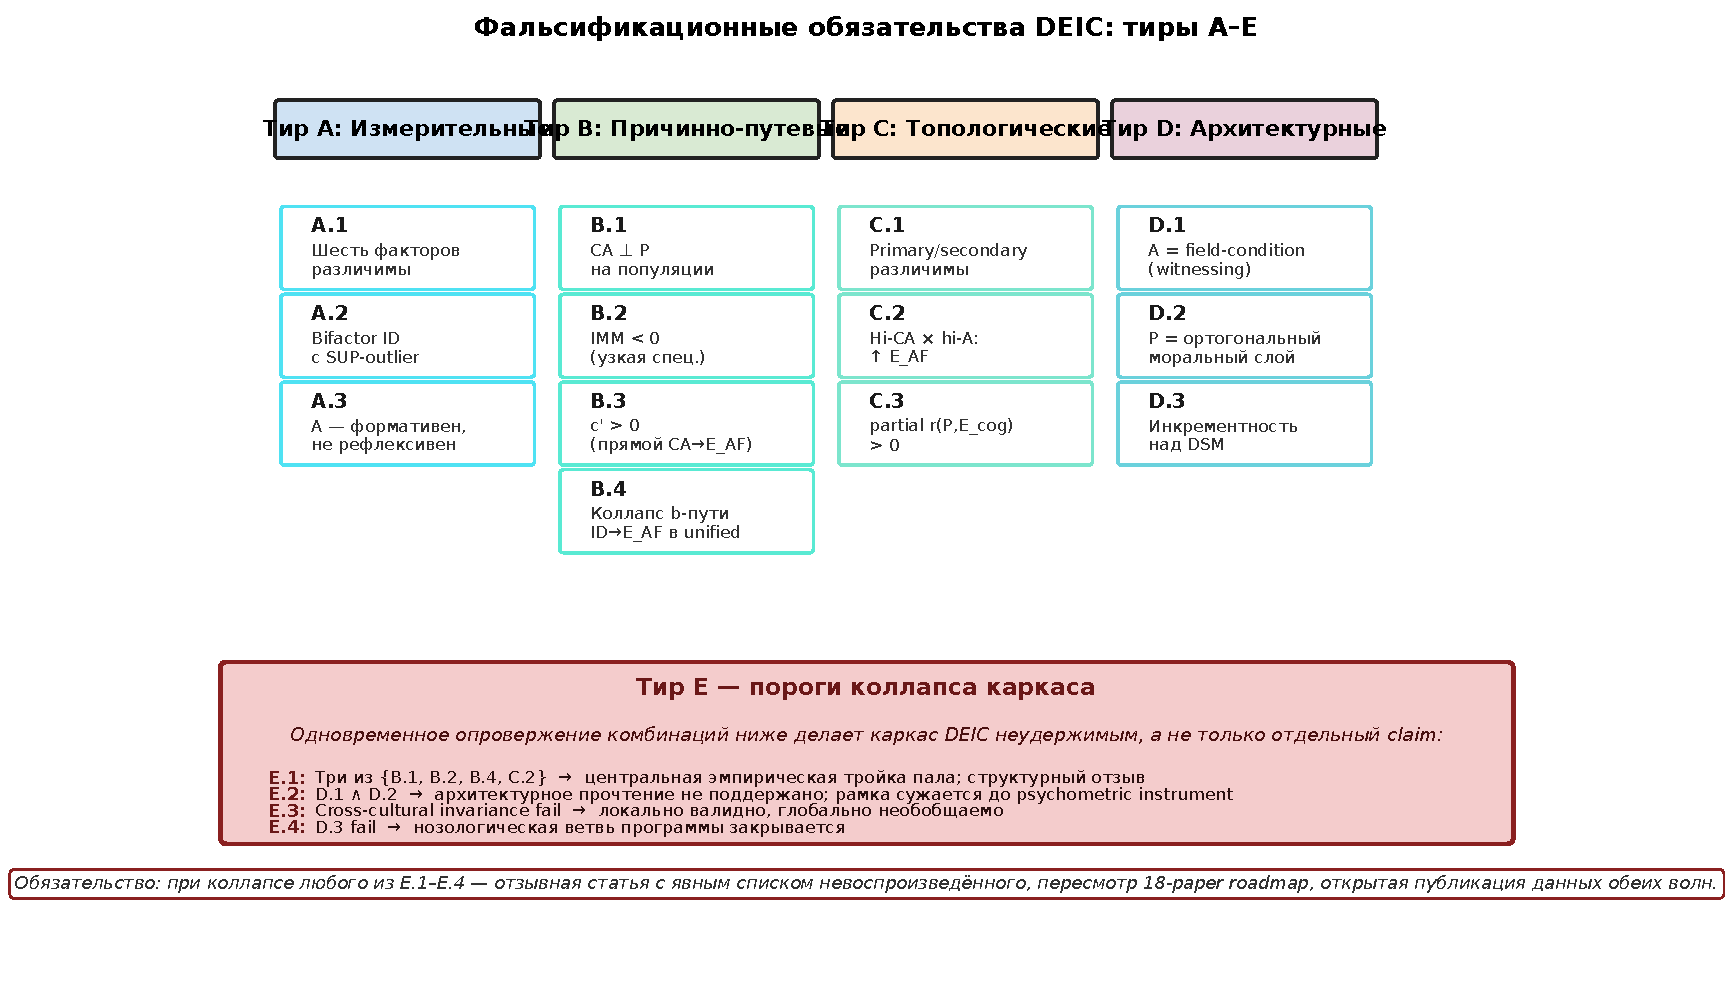
\includegraphics[width=0.95\linewidth]{figures/fig10_falsification_map.pdf}
\caption[Map of falsification commitments]{Map of \DEIC{}'s falsification commitments. Four tiers of local tests (A --- measurement; B --- causal paths; C --- topology; D --- architecture) form the upper row, each with its own commitments. The lower red band --- Tier~E: programmatic collapse thresholds at which the scaffolding is subject to structural revision rather than local update.}
\label{fig:falsification_map}
\end{figure}

The formulations are deliberately binary. Science does not work in binary modes --- but commitments do: either we are prepared to recognize a result as refutation, or we rule it out of the test ahead of time, in which case it is not a commitment.

\subsection{Tier A: measurement commitments}
\label{subsec:falsification_tier_a}

\paragraph{A.1 --- Six factors are distinguishable.}
\emph{Claim.} The six-factor oblique CFA (ID, CA, P, M, \EAF{}, \Ecog{}) is robustly reproduced on pre-registered items designed to separate the constructs.
\emph{Falsifier.} In wave~2, with items separated by design ($N \geq 1000$), either \EAF{} and \Ecog{} merge into a single empathy factor (CFI of the model with combined E is no worse than with separated by $\Delta$CFI $\leq 0.01$), or ID and CA are indistinguishable as separate latents ($r_{\mathrm{lat}} > 0.90$), or P and M are indistinguishable under instrumental independence.
\emph{Test requirements.} Pre-registered design; items for \EAF{} and \Ecog{} written on different content-specific constructs, not sharing common words. $N \geq 1000$ for stable CFA on 6 factors.
\emph{Consequence of refutation.} The multidimensional architecture of empathy in its current form is not supported; \DEIC{} narrows to the factor structure the data sustain (possibly four- or five-factor).

\paragraph{A.2 --- Bifactor structure of ID with SUP as separate.}
\emph{Claim.} The ID umbrella is better described by a bifactor model (general ID$_{\mathrm{g}}$ plus five uncorrelated specific factors) than by a unidimensional one, under $\Delta\chi^2$ at $p < 0.001$. Per-subscale ECV for SUP remains below $0.45$, for FLA above $0.70$.
\emph{Falsifier.} In wave~2 the bifactor model does not exceed the unidimensional one under $\Delta\chi^2$ at $p < 0.01$, OR ECV for SUP $> 0.55$ (SUP is equally well absorbed by general ID), OR ECV for FLA $< 0.45$ (FLA ceases to be a pure indicator of general ID).
\emph{Test requirements.} $N \geq 1200$ with items for SUP reconstructed as a standalone latent by design in wave~2.
\emph{Consequence of refutation.} The hypothesis that ``passive blocking is a single architecture with surface variations'' is revised; re-segmentation of ID into two independent latents is possible.

\paragraph{A.3 --- A is formative, not reflective.}
\emph{Claim.} A in the current instrument works as a formative composite. A dedicated A-scale, designed to isolate witnessing (observation-of-observation without trauma hypervigilance), will yield a reflective unifactorial CFI $\geq 0.93$ and reproduce a negative \IMM{} in the narrow specification.
\emph{Falsifier.} A dedicated witnessing-A-scale yields a single-latent CFI $\geq 0.95$ \emph{and} an \IMM{} that reproduces the sign and direction of the composite $-0.00197$ (CI does not include zero) --- then A is reflective, and our argument for its formativity is false. Or, conversely, the witnessing scale yields CFI $< 0.85$ and non-significant \IMM{} --- then neither operationalization of A supports the witnessing-moderation hypothesis.
\emph{Test requirements.} Item-level separation of witnessing (Josipovic/Dunne/Grabovac-anchor items) and hypervigilance (trauma-focused items); $N \geq 800$; nested conditional-process SEM.
\emph{Consequence of refutation (either branch).} Either A is reinterpreted as a reflective construct (simplification), or the witnessing-moderation hypothesis is not supported (revision of the central claim about the role of attention).

\subsection{Tier B: causal-path commitments}
\label{subsec:falsification_tier_b}

\paragraph{B.1 --- CA$\perp$P at the population level.}
\emph{Claim.} In the parallel mediation CA$\to$\{ID, P, M\}$\to$\EAF{}, the CA$\to$P path remains close to zero ($|\beta| < 0.10$) in a replication with a sample comparable in CA-spectrum breadth.
\emph{Falsifier.} CA$\to$P $\beta > 0.20$ at $p < 0.01$ in a replication sample $N \geq 1000$ with a CA-instrument and P-instrument of comparable content.
\emph{Test requirements.} Replication on an independent sample; the CA-instrument covers the same spectrum (early relational neglect, abuse, emotional deprivation); the P-instrument preserves the proportion of moral and architectural signature.
\emph{Consequence of refutation.} Architectural orthogonality of P and CA is not supported; primary and secondary psychopathy become a continuum rather than topologically separate cells. Clinical consequence: the psychopathic pattern is reinterpreted as a (co-)outcome of childhood trauma, not a separate architecture.

\paragraph{B.2 --- \IMM{} in the narrow specification is negative.}
\emph{Claim.} In the conditional-process SEM without P in the $b$-equation, the \IMM{} of the CA$\to$ID$\to$\EAF{} channel is negative, with 95\% CI not including zero.
\emph{Falsifier.} $P(\mathrm{IMM} < 0) < 0.90$ under any of the three reference Bayesian priors on a replication sample, OR the CI of the frequentist estimate crosses zero at $N \geq 1000$ with comparable A-composite structure.
\emph{Test requirements.} A-composite with comparable weighting structure; replication conducts parallel Bayesian and frequentist analyses.
\emph{Consequence of refutation.} The central result of the paper (two-stage A-moderation of CA$\to$ID$\to$\EAF) is not supported; A as moderator of the channel in the narrow specification is revised.

\paragraph{B.3 --- $c'$ (direct path CA$\to$\EAF{}) is positive.}
\emph{Claim.} After partialling ID, P, M and A, the direct path CA$\to$\EAF{} remains positive ($+0.15$--$+0.25$) --- ``raw'' childhood trauma does not kill empathy by itself; the defensive cascade kills it.
\emph{Falsifier.} $c' < -0.10$ with $p < 0.01$ in a replication, after correct partialling.
\emph{Test requirements.} Replication preserving the mediator structure; control for response bias (Lie as a covariate of \EAF).
\emph{Consequence of refutation.} The key thesis of the introduction (``trauma is not a verdict; defense transmits it'') loses its empirical footing; the \DEIC{} framework shifts to the more standard ``trauma $\to$ emotional damage'' narrative.

\paragraph{B.4 --- In the unified SEM the $b$-path ID$\to$\EAF{} collapses.}
\emph{Claim.} With all paths estimated simultaneously in the unified SEM the ID$\to$\EAF{} coefficient drops to statistical non-significance ($|\beta| < 0.10$, $p > 0.05$), and P$\to$\EAF{} dominates.
\emph{Falsifier.} In replication, the $b$-path ID$\to$\EAF{} remains $\beta < -0.20$ at $p < 0.001$ even with P included in the same equation.
\emph{Test requirements.} Replication of the unified SEM with the same latent structure.
\emph{Consequence of refutation.} The separation of ``architectural'' and ``narrative'' layers in the $E_{\mathrm{AF}}$ model is not supported; P and ID turn out to be additive rather than hierarchical mediators, and the theoretical separation of orthogonal channels requires revision.

\subsection{Tier C: topological commitments}
\label{subsec:falsification_tier_c}

\paragraph{C.1 --- Primary and secondary psychopathy are topologically distinguishable.}
\emph{Claim.} In the hi-P subsample ($N \geq 200$) bimodality is observed along the ID axis (or, in a multidimensional version, two distinct clusters in the ID$\times$CA plane), corresponding to the Karpman distinction: a primary cell (ID $\approx 0$, CA $\approx 0$) and a secondary cell (ID $> +0.5$, CA $> +0.5$).
\emph{Falsifier.} In the hi-P subsample $N \geq 200$ the Hartigan dip test gives no evidence of bimodality ($p > 0.1$), OR a Gaussian mixture on (ID, CA, A) gives a better BIC for $k=1$ than for $k=2$.
\emph{Test requirements.} Replication on an independent sample; preferably clinically enriched with a hi-P subgroup.
\emph{Consequence of refutation.} The Karpman distinction on \DEIC{}-coordinates is not supported; the topological $2\times2$ collapses into continuum psychopathy, as in much of contemporary literature. Clinical consequence: different interventions for ``primary'' and ``secondary'' types lose their footing.

\paragraph{C.2 --- The integrated survivor has elevated \EAF{}.}
\emph{Claim.} The hi-CA $\times$ hi-A cell ($\geq$ medians on each axis; expected share $\sim 15$--$18\%$ of the sample) has \EAF{} exceeding the median of the overall sample and exceeding the hi-CA $\times$ lo-A cell by at least $0.4\sigma$.
\emph{Falsifier.} $\mathrm{mean}\ \mathrm{E_{AF}}$ in the hi-CA $\times$ hi-A cell is at or below the overall sample median ($\Delta \leq 0$), OR the difference from hi-CA $\times$ lo-A $< 0.2\sigma$ in a replication $N \geq 1000$.
\emph{Test requirements.} Replication with analogous operationalization of A (composite or an equivalent witnessing scale); sample includes sufficient hi-CA representation ($\geq 25\%$).
\emph{Consequence of refutation.} The central publicly-significant claim that witnessing work compensates for the CA effect on affective empathy is not supported; ``trauma is not a verdict'' as an empirical claim is withdrawn and remains as a clinical horizon without statistical footing.

\paragraph{C.3 --- Partial $r$(P, \Ecog) is positive.}
\emph{Claim.} After partialling ID and CA, the partial correlation of P and \Ecog{} remains positive ($> +0.15$). This is explained by hyper-instrumentation: the P-pattern uses recognition of others' states selectively and is not deficient on the cognitive-E axis.
\emph{Falsifier.} Partial $r$(P, \Ecog{} \textbar{} ID, CA) $\leq 0$ in a replication $N \geq 1000$ with comparable separation of \EAF{}/\Ecog{}.
\emph{Test requirements.} The \Ecog{} scale is written on perspective-taking and understanding-of-others, not on empathic concern; the P-scale preserves the moral and architectural proportions; items do not share words.
\emph{Consequence of refutation.} The hyper-instrumentation hypothesis of Blair/Baron-Cohen is not reproduced in our data; the ``classical'' description of psychopathy as deficient on both forms of empathy turns out to be more accurate. The framing ``architecture, not deficit'' on the E axis weakens.

\subsection{Tier D: architectural commitments}
\label{subsec:falsification_tier_d}

\paragraph{D.1 --- A as field-condition, not as content of the field.}
\emph{Claim.} A dedicated witnessing-A-scale, separated by design from trauma hypervigilance, gives the same sign and direction of channel moderation CA$\to$ID$\to$\EAF{} as the current A-composite. If, however, a pure hypervigilance scale is constructed (attention-to-the-internal only, without witnessing), it moderates the channel in the opposite direction or does not moderate it at all.
\emph{Falsifier.} Both scales (witnessing-only and hypervigilance-only) moderate the channel in the same direction in a replication, OR the witnessing scale does not moderate at all.
\emph{Test requirements.} Two parallel item sets, content-validated by experts in contemplative tradition and trauma psychology; the same SEM structure for both.
\emph{Consequence of refutation.} The ontological distinction witnessing vs content at the attention axis is not supported; A returns to the general ranks of components of dispositional attention; the connection to the non-dual contemplative tradition loses empirical footing (it remains theoretical).

\paragraph{D.2 --- P as orthogonal moral layer.}
\emph{Claim.} Cognitively-morally phrased P-items (``I believe that in my case such behavior is permissible'') yield $\beta$ on \EAF{} and partial correlations with architectural-P-items such that the P-composite preserves $\approx$ half its variance as a moral component and $\approx$ half as architectural. P-moral alone remains orthogonal to CA ($|\beta| < 0.10$).
\emph{Falsifier.} After separating P into P-moral and P-arch in wave~2 both components either have $r_{\mathrm{lat}} > 0.85$ (indistinguishable), or P-moral correlates with CA at $\beta > +0.25$.
\emph{Test requirements.} Pre-registered item split; $N \geq 1000$; explicit cognitively-moral vs architectural phrasings.
\emph{Consequence of refutation.} The moral layer of P is not distinguishable from the architectural one; the interpretation of psychopathy as ``conditional coupling plus narrative of permission'' becomes internally inoperable and reduces to a single architectural component. The ethical framing ``architecture is morally neutral; narrative is evaluable'' loses its empirical cut-off.

\paragraph{D.3 --- Incremental validity of the \DEIC{} profile over the DSM label.}
\emph{Claim.} In retrospective re-analysis of clinical datasets with treatment response as outcome, the baseline \DEIC{} profile explains at least 5\% of additional variance in response after partialling out the DSM label.
\emph{Falsifier.} In retrospective on clinical data $N \geq 2000$ with measured \DEIC{} profile, incremental $R^2$ over DSM $< 0.05$.
\emph{Test requirements.} One or more clinical samples with parallel \DEIC{} measurement and DSM diagnosis; outcome: treatment response on a standardized metric (HAMD, PHQ, BDI, etc.).
\emph{Consequence of refutation.} The nosological claim of \DEIC{} as a trans-diagnostic stratifier is not supported; the framework narrows to a descriptive-theoretical role without a claim to clinical reorganization.

\paragraph{D.4 --- DI as an architectural marker, not an indicator of social desirability.}
\emph{Claim.} The magnitude of the declarative--behavioral gap $DI_{overall}$ tracks the defensive latent ID ($r \geq +0.30$) and the witnessing latent A ($r \leq -0.30$), and does not track clinical diagnosis ($|r| < 0.15$) in wave 2 on an independent sample. The prosocial-aligned version $DI_{aligned}$ remains structurally distinct from $piz$ ($|r| < 0.50$ with a sign opposite to the one expected were DI a self-presentation indicator).
\emph{Falsifier.} In wave 2 ($N \geq 800$), either $|r(DI_{overall}, \text{ID})| < 0.30$, or $|r(DI_{overall}, \text{dx\_any})| > 0.20$, or $r(\text{piz}, DI_{aligned}) > +0.30$ (turning DI into a sub-component of $piz$ without an independent disposition).
\emph{Test requirements.} Wave-2 inventory preserving the principle of paired declarative/behavioral formulations on all scales of the ID perimeter; re-measurement of dx and $piz$ on the same sample; re-fit of the 6-factor oblique CFA with latent scores.
\emph{Consequence of refutation.} DI as an independent architectural metric is not supported: either the gap does not track architecture, or it tracks the clinical profile (which moves DI into a diagnostic rather than architectural category), or it is fully explained by $piz$ (a pure SD artifact). In any of these cases, §\ref{subsec:di_asymmetry} and the interpretation of DI in §\ref{subsec:di_results} require retraction; \texttt{extended\_metrics.DI} in the instrument moves from an architectural marker to either a clinical one or a duplicate of $piz$, and its place in the wave-2 dashboard is reconsidered.

\subsection{Tier E: programmatic collapse thresholds}
\label{subsec:collapse_thresholds}

Up to this point each commitment has been described as a local test with a local consequence. But \DEIC{} is not a set of independent hypotheses --- it is an architecture with interdependent nodes. Refutation of certain combinations means that the scaffolding as a whole does not hold, and not merely that one branch has grown stale. We formulate these combinations explicitly.

\paragraph{E.1 --- Collapse of the central empirical triad.}
If three of the four central commitments are simultaneously refuted --- B.1 (CA$\perp$P), B.2 (\IMM{} negative), B.4 (collapse of $b$-path in unified), C.2 (integrated survivor with elevated \EAF) --- three of the empirical pillars on which the central argument of the paper is built are not reproduced. In that case \DEIC{} as an empirical framework requires \emph{structural revision, not update}: instrument version~2 and the accompanying theoretical framework must be retracted and replaced by a narrower working hypothesis with explicit indication of those fragments that at this point remain supported.

\paragraph{E.2 --- Collapse of the architectural reading.}
If D.1 (witnessing-moderation) and D.2 (distinguishability of P-moral and P-arch) are simultaneously refuted, the theoretical framework ``psychopathy as conditional coupling plus moral narrative; attention as field-condition'' is not supported. \DEIC{} in that case \emph{narrows to an empirical coordinate system} without architectural or ontological theses: fit for use as a psychometric instrument, but not as a framework claiming dialogue with the contemplative tradition and with moral philosophy.

\paragraph{E.3 --- Collapse of generalizability.}
If cross-cultural validation on non-Russian-speaking samples (EN, ES, CH, AR) shows that the six-factor CFA does not reproduce scalar invariance, and the central B.2 and C.2 reproduce only in \emph{part} of the cultural contexts, \DEIC{} remains a \emph{locally valid, globally non-generalizable} instrument. This is not a collapse of the framework as such, but a withdrawal of the claim that the described architecture is a universal device of the psyche rather than an artefact of Russian-language/late-Soviet cultural formation. The applied papers of the program (political communication, evolutionary psychology) are in that case restricted to the corresponding cultural range.

\paragraph{E.4 --- Collapse of the nosological claim.}
If D.3 (incremental validity over DSM) is refuted, the nosological branch of the program (the paper on the \DEIC{} profile as trans-diagnostic stratifier, §\ref{sec:future}) is closed until new grounds emerge. The framework remains descriptively scientific, but without claim to reorganization of clinical categories.

\paragraph{What ``the scaffolding is subject to revision'' means.}
We acknowledge: public retraction or structural revision is not the same as silence. In the event of collapse of any of levels E.1--E.4 we commit to \textbf{(i)}~publish a retraction paper with an explicit list of what is not reproduced and with an explicit reformulation of what remains; \textbf{(ii)}~revise the 18-paper publication roadmap --- some of the planned papers will lose their grounds and be withdrawn; \textbf{(iii)}~publish the data of both waves openly, so that other groups can conduct independent re-analyses. This commitment has the same form as the commitments of open methodological culture after the replication crisis in social psychology of the 2010s: not ``if we are wrong, we will rewrite history'', but ``if we are wrong, we will acknowledge it and release the data''.

\subsection{What this section means for reading the paper}
\label{subsec:falsification_closing}

We draw two consequences for the reader.

First. No statement in this paper should be read as a ``closed'' or ``proven'' fact. Each is a hypothesis with its own falsification boundary, formulated here. In the body of the paper --- in Results, in Discussion --- these statements are formulated in the findings register (``the data show'', ``the model yields''), as psychometric reporting requires. But the scientific status of each is determined not by that register, but by the presence of a formulated falsifier in this section.

Second. We do not regard falsification as a threat to the program. Refutation of a local prediction (any of A.1--D.3) is a normal course of empirical inquiry and a basis for an update. Refutation of a combination (E.1--E.4) is a normal course of scientific self-correction, and the program foresees this outcome as a possibility. The only outcome unacceptable to us is not refutation, but evasion: if statements are formulated such that they cannot be either confirmed or refuted, the work falls outside the boundaries of science regardless of its technical sophistication. The falsification section exists precisely to prevent such evasion. This --- a contribution we consider independent of whether the framework itself turns out to be valid.

In §\ref{sec:future} we formulate the concrete designs that will carry out each of the tests. In the open documentation of the program (\texttt{PROGRAM\_STRUCTURE.md}) the planned papers are listed with their mapping to Tiers A--E of this section.

\section{Limitations}
\label{sec:limitations}

The present work carries a number of limitations, organized here along four axes: epistemological, measurement, design, statistical. These are not retrospective hedges on the claims but an explicit boundary of what the data support and what they do not.

\subsection{Worldview as the primary source of the frame}
\label{subsec:worldview_first}

The DEIC program is built \emph{worldview-first}, and we take it as obligatory to name this order openly. The picture of how the architecture of empathy and non-empathy is organized crystallized for the authors before the data were collected --- out of psychoanalytic tradition, clinical observation, and the material of contemplative sources; the 131-item instrument was constructed specifically to test that picture. This is not an anti-pattern: most substantive theoretical syntheses in psychology (attachment theory in \citealp{bowlby1969}, mentalization theory in \citealp{fonagy2002}, the clinical tradition of psychopathy from \citealp{cleckley1941} to \citealp{hare1991}) are built in exactly the same way, and ``data first, theory second'' remains a rhetorical posture that rarely matches the actual process. We consider it more honest to name this order than to disguise it as the reverse.

Three specific risks follow from the worldview-first structure, and each requires explicit disclosure.

\paragraph{Confirmation risk.} The author of the frame has freedom in the choice of instrument, model specifications, aggregation methods, and interpretation, and may unconsciously optimize these decisions to confirm the initial intuition. The defense is pre-registered replication on an independent sample, collected and analyzed by a researcher not involved in the development of the frame and methodologically inclined to refute it. Without this step the present work must be read as an extended hypothesis, supported by one well-developed sample, rather than as an established fact.

\paragraph{LLM as a structural amplifier of the frame.} A substantial part of the work on refining constructs, formulating theoretical connections, and composing the final scaffolding was carried out in dialogue with large language models. This is methodologically significant not because of hallucinations (negligible in conceptual work) but because of the asymmetry of resistance. An LLM without its own biography, without a defensive structure, and without a source of skepticism outside the frame it is given is not a skeptical colleague but a logically coherent resonator: it extends the author's original frame into regions where a live interlocutor would stop and say ``wait''. The absence of friction here is not the absence of correction but active amplification. Partial compensation --- live disputation with a methodologically sober opponent not sharing the frame --- must be built into the preparation of wave 2 and explicitly recorded in methodology.

\paragraph{Three cardinal falsification conditions.} A frame is meaningful only if it pays a price. We formulate three cardinal conditions the failure of which destroys the corresponding parts of the program.

\emph{(a) Age-invariance of the CA$\to$ID$\to$\EAF{} channel in the 14--45 range.} If in an independent replication the parameters of the channel depend significantly on age within this range, the claim about a critical window of architectural formation closing before age 14 does not hold, and the entire architectural--ontogenetic interpretation of the program loses its ground.

\emph{(b) Orthogonality P$\perp$CA at the population level.} If in replication the correlation of P with CA is significantly positive, or the indirect effect CA$\to$P$\to$\EAF{} is significantly non-zero, the two-layer structure of P (architecture $+$ moral narrative, independent of childhood history) does not hold, and the model reverts to the standard clinical frame ``psychopathy as a consequence of trauma''.

\emph{(c) Reproducibility of the primary cluster (hi-P, lo-CA, lo-ID).} In the present data it was isolated by rule-based classification at $n = 144$ (10\% of the sample). If in an independent replication this cluster is not isolated or its size is radically smaller, the distinction between primary and secondary patterns returns to the status of a theoretical conjecture, and the claim of two etiological routes into the conditional architecture is not supported.

These three conditions are not a symbolic gesture but a real costly wager: the failure of any one of them will require a reformulation of the central part of the frame. Together with the three points of empirical resistance already observed in the present sample (§\ref{subsec:data_resistance_en}), they form the minimal set of tests that makes DEIC a falsifiable program rather than a self-confirming frame.

\subsection{Measurement limitations}

\paragraph{A as a formative, not reflective, construct.} This limitation is confirmed empirically in A-CFA Tier 5. On 17 carefully selected metacognitive items, CFI $= 0.866$, RMSEA $= 0.081$, $\omega$ by absolute loadings $= 0.947$, but the loadings are \emph{bipolar}---8 positive, 9 negative after external polarity alignment. When this latent A is substituted into conditional process SEM, the signs reverse relative to the theoretically weighted composite (A$_{\mathrm{lat}} \to$ ID $= +0.66$ against the composite's $-0.63$), and \IMM{} $= -0.00044$ [$-0.00267, +0.00052$] is nonsignificant. This is not a failure of analysis but empirical proof that the current item pool does not distinguish witnessing (observing-observation) from trauma hypervigilance (a pathological hypervigilance toward inner states). The main composite works because we built this distinction into the weights in advance. A dedicated A-scale is priority number one for wave 2.

\paragraph{M factor of low reliability.} $\omega = 0.546$ against $\omega > 0.89$ for the other five factors. Masking is weakly differentiated from P ($r_{\mathrm{latent}} = +0.82$). M-specific claims are not made in the paper; M is kept as a regulatory layer to be rebuilt in wave 2.

\paragraph{Post-hoc status of the ACE extension.} The extension of the ACE construct (treating ``don't remember / don't know'' as a positive signal of an adversity-relevant family or cognitive configuration rather than as missing data) is discussed substantively in §\ref{subsec:ace_extension} and validated on wave 1 through a full 6-factor oblique CFA re-fit (N~$=$~1468 against canonical 1426; CFI~$=$~0.960, RMSEA~$=$~0.062; bootstrap 95\,\% CIs of the indirect effects do not cross zero). Nevertheless this validation is \emph{post-hoc}: the recoding and re-fit were performed after the original publication CFA. A pre-registered wave 2 with an initially designed ACE-dissociation subscale and stated criteria in advance (McDonald's $\omega \ge 0.7$, $r(\text{ACE-dis}, \text{ID}_{\mathrm{lat}}) \ge 0.30$) is the condition for turning the extension from an observation into a claim about a reproducible structure. See §\ref{sec:future}.

\paragraph{Collapse of wave-1 scales into the present six-factor structure.} The progenitor instrument (DEIC-Inventory wave 1) had 12 content scales $+$ 2 controls (A, Lie). The published six-factor oblique CFA model is the result of two psychometrically forced collapse operations and one split operation.

\emph{Collapse of defenses (five into one, preserving the conceptual center).} Wave 1 had five scales of passive blocking: four mechanism-specific---suppression (\texttt{S}), dissociation (\texttt{D}), affective isolation (\texttt{AIS}), affective flatness (\texttt{F})---and one experientially central, the \emph{Internal Dissonance Scale} (\texttt{IDS}), measuring the subjective experience ``an empathic response began but does not continue; I want to feel but I cannot.'' The choice of a single ID latent in the main model is a decision of \emph{parsimony}, not a verdict on the structure: on our data the five-factor oblique CFA converges (CFI~$=$~0.891, RMSEA~$=$~0.077), but the latent correlations among the five defenses have $|r|$ in the range $0.66$--$0.89$ with partially opposite signs (a structure of mixed signs characteristic of semi-collapsed collinearity). At this level of separability the five separate latents do not yield a clinically or statistically stable distinction; meanwhile, a common ID latent absorbs most of the variation. Wave 2 (the present work) preserves the conceptual center unchanged and simply removes ``Scale'' from the label: \texttt{IDS} $\to$ \textbf{ID} (\emph{Internal Dissonance}). The extension consists in the fact that the four mechanism-specific scales (S, D, AIS, F) are absorbed into the same latent as surface manifestations of a single field. Substantively this agrees with Fonagy (the absence of a mentalizing field as a condition, not a sum of mechanisms) and with Di Giuseppe \& Perry \citep{digiuseppe2024} (defenses as an integrated network rather than parallel traits).

\emph{Limitation of parsimony.} Absorption is not equivalent to proof of unidimensionality. In an additional bifactor analysis (§\ref{subsec:id_bifactor}), a general factor model (ID\textsubscript{g} plus five uncorrelated specific factors) exceeds the unifactor ID model on the principal indices and shows that the general ID explains about 57\,\% of the total variance (ECV\textsubscript{global}~$=$~0.57), with notable per-subscale heterogeneity: FLA and IDS are almost fully absorbed by the general ID (ECV~$=$~0.86 and 0.66 respectively), DIS and AIS retain about half of their unique variance (ECV~$\approx$~0.54, 0.53), while SUP remains to a significant degree a separate construct (ECV~$=$~0.31). Clinically this means: suppression (SUP) is the worst-absorbed by the umbrella latent, and in wave 2 should with high probability be restored as a separate latent; FLA, on the contrary, is well described by the general ID and can remain a reliable indicator of it; DIS and AIS stand in between---they require either additional items for clean separation or a bifactor level in the published model. The phenomenological distinctions among surface mechanisms---suppression (ego-syntonic, conscious), dissociation (ego-dystonic, automatic), affective isolation (content present, feeling severed), flatness (affective signal absent)---are hidden in the published unifactor ID model; in the bifactor model and in the wave-2 design they are restored.

\emph{Collapse of the contextual layer (ACE $+$ CA $\to$ CA).} Wave 1 distinguished a general index of adverse childhood experiences (\texttt{ACE} in the spirit of Felitti et al.) and a narrow scale of childhood adversity (\texttt{CA}, with an emphasis on early-years relational trauma). In our sample these turned out to be interchangeable indicators of one latent ($r > 0.8$), so the published model uses a single \textbf{CA} as the latent of early relational-stress history. The wave-1 distinction among types of trauma (domestic violence, emotional deprivation, attachment instability) is hidden in this aggregation. Additional wave-1 contextual scales---emotional context (\texttt{EC}) and an affective-dissociative indicator (\texttt{ADI})---are retained as observed composites for descriptive use but do not enter the main CFA as latents.

\emph{Split of empathy (one into two).} The opposite operation: the wave-1 general empathy scale \texttt{E} was split into \EAF{} and \Ecog{} post-hoc, in response to the P$\leftrightarrow$E paradox in the original model and in agreement with the multidimensional tradition of Davis \citep{davis1983}. This is an acquisition, not a loss; but it is post-hoc and must be reproduced on pre-registered items separated by design (see below---statistical limitations).

\begin{figure}[htbp]
\centering
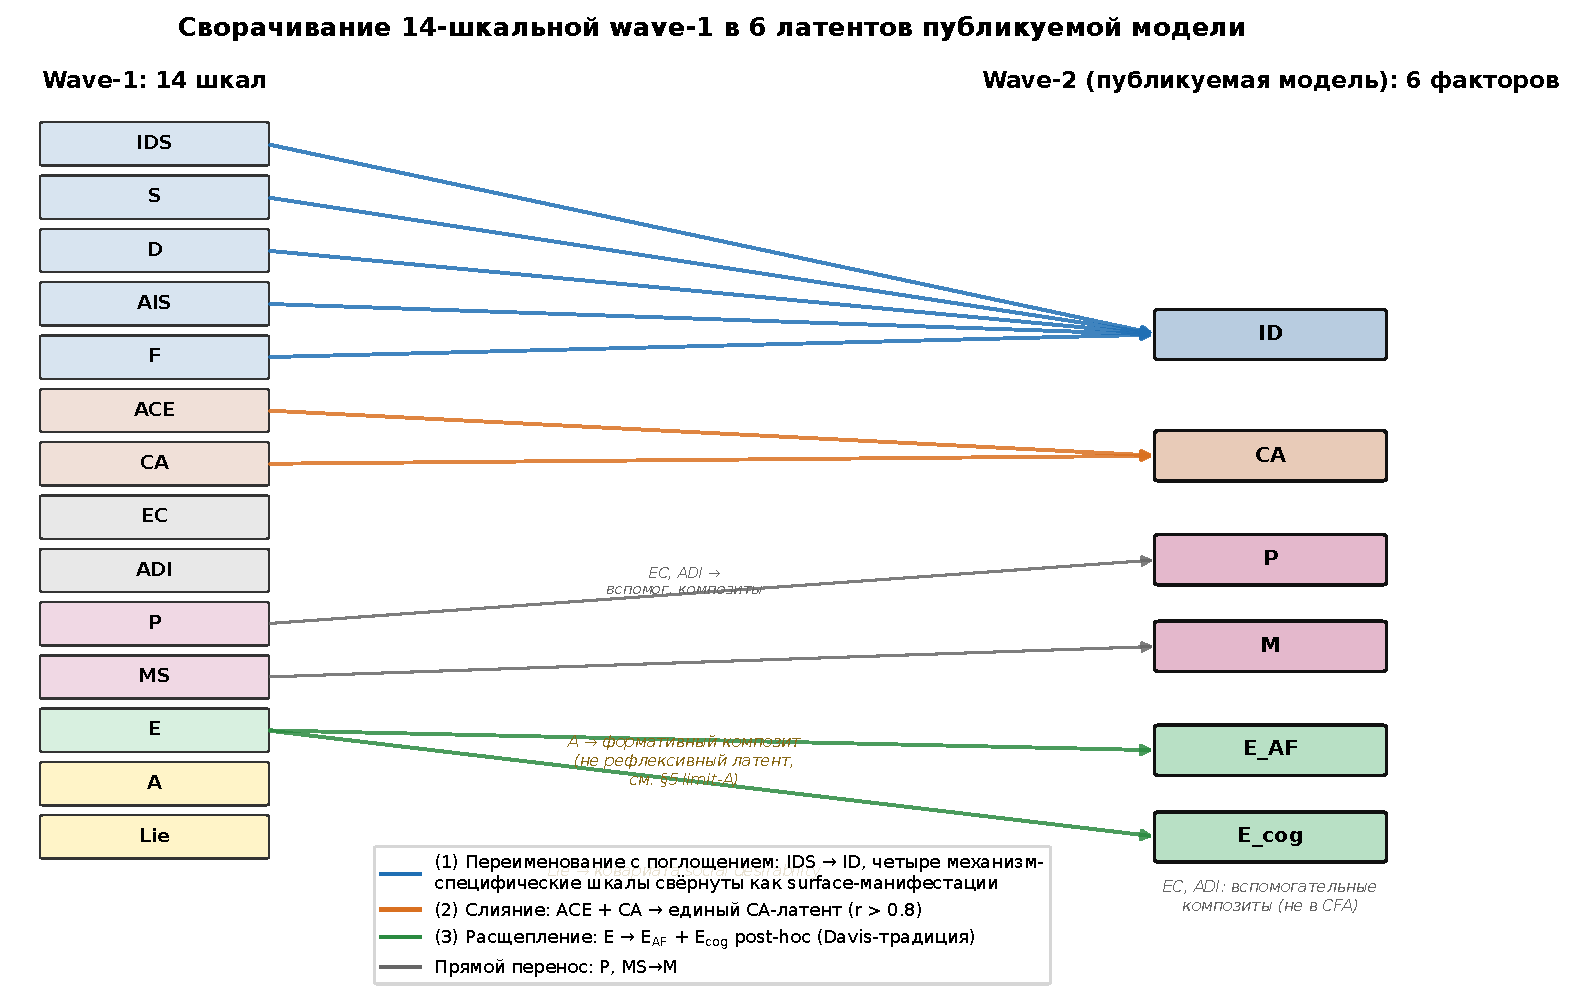
\includegraphics[width=0.95\linewidth]{figures/fig9_wave_mapping.pdf}
\caption[Wave-1 to wave-2 transition map]{Map of the transition from 14 wave-1 scales to 6 latents of the published model. Blue arrows: renaming with absorption (IDS $\to$ ID, together with S, D, AIS, F as surface manifestations of one field); orange: merger of two indicators of early history (ACE + CA $\to$ CA); green: split of the general empathy scale (E $\to$ \EAF{} + \Ecog{}); gray: passthrough (P, MS $\to$ M). EC, ADI retained as auxiliary observed composites; A, Lie---control scales.}
\label{fig:wave_mapping}
\end{figure}

\emph{Resulting map.} 12 wave-1 content scales $\to$ 6 latents of the published model: \texttt{IDS} $\to$ \textbf{ID} (renaming with absorption of \{\texttt{S, D, AIS, F}\} as inseparable surface manifestations of the same field); \{\texttt{ACE, CA}\} $\to$ CA (merger of two indicators of early relational history into a single latent); \texttt{P} $\to$ P; \texttt{MS} $\to$ M; \texttt{E} $\to$ \{\EAF, \Ecog\} (post-hoc split, the only expansion operation); \{\texttt{EC, ADI}\} $\to$ auxiliary observed composites. A is separated as a formative composite; Lie is a social-desirability covariate correcting E and ID in the applied integral metrics. The published six-factor structure is the minimal one the data support. The phenomenological and typological distinctions hidden by that minimality are a task for wave 2.

\paragraph{Multi-scale weights in \texttt{questions.json}---an innovation and its scoring artifact.} The explicit a priori assignment to each item of a vector of weights across several factors is a substantive innovation of the instrument, not a methodological carelessness: most empathy questionnaires pretend that simple structure holds and assign an item to a single scale, losing the share of variance that sits at the intersections of constructs. DEIC brings this cross-structural aspect out of implicit statistical artifact and into an explicit theoretical declaration that can be criticized and validated (its closest psychometric relative is the a priori bifactor model). However, composite sum-scoring with multi-scale weights algebraically inflates correlations among composites: an item with nonzero weights in two composites is counted on both sides of the equation when those composites correlate. In our sample the average inflation is $\sim 0.18$, with a maximum of $0.68$ with a sign change for P$\leftrightarrow$E. Latent factor scores are immune to this problem because CFA correctly partitions common and specific variance. The wave-2 solution is not the abandonment of the innovation but its separation into two independent layers in \texttt{questions.json}: \texttt{factor\_weights} (a vector for CFA with explicitly prescribed cross-loadings---the theoretical layer remains) and \texttt{primary\_scale} (the single factor for composite sum-scoring---one item, one composite). Composites are published as orienting without algebraic inflation; latent scores as the main scientific result. The innovation is retained in full and becomes two-layered by construction.

\paragraph{Self-report only.} No informant report, no behavioral measures, no physiological convergent measures. Especially critical for A, where self-report has a circular-validity limitation (an accurate report on attention requires attention).

\paragraph{The secondary psychopathic subgroup is small.} $n = 65$. Rule-based $2 \times 2$ yields a stable direction, but effect sizes in the secondary cell have wide CIs and require a clinical sample for confirmation.

\subsection{Design-related limitations}

\paragraph{Cross-sectional.} No temporal axis, no pre/post therapy design, no retest stability. Consequence: it is impossible to distinguish stable A from transient A, impossible to test the longitudinal predictions formulated in §\ref{subsec:falsifiers}, and impossible to distinguish empirically the direction of causation in the CA--ID pair (assumed theoretically but statistically unidentified).

\paragraph{Monolingual sample.} Russian-language internet recruitment; a self-selected sample. Cultural, linguistic, and platform biases are present. Cross-cultural validation (EN, ES, CH, AR) with invariance testing is the obligatory next step.

\paragraph{Age skew} toward 18--37; the 38$+$ subsample ($n = 50$) is small. Suppressor mediation is stable at 18--37 and weakens at 38$+$; the mechanism is unclear---post-therapy effects, survivor bias, developmental shift---and requires an age-stratified sample.

\paragraph{Self-selection through Telegram/VK.} The survey requires an introductory metacognitive vocabulary; possibly this form of selection already shifts the A distribution to the right relative to the general population. The data do not support generalization to non-reflective subpopulations.

\paragraph{The ``befriends-psychopaths'' subsample and individual-level ethics.}
\label{subsec:limitations_befriends}
The archetype of the empathic counterpart in a dyad with a psychopath (hi-E $+$ hi-P in the $+++-$ octant) is empirically confirmed but represented in the sample by only $n = 3$ respondents ($0.19\,\%$). None of them endorsed any free-text diagnostic category; self-descriptions of this profile in the open field are absent: the archetype is systematically invisible to self-report. Retrospective power estimate: detection of $d = 0.5$ in this subgroup requires $n \approx 150$; $d = 1.0$---$n \approx 30$. In the present wave the profile is recorded descriptively, without parametric comparisons. Wave 2 requires targeted sampling of this configuration. \emph{Ethical limitation:} one of the three respondents is known to us biographically; therefore any individual-level characteristics of this subgroup are published only as aggregated centroids ($n = 3$), and individual-level data from the paper is excluded and not released to the open supplementary.

\subsection{Statistical limitations}

\paragraph{Multivariate non-normality of the data and robust fit indices.} Mardia $p < 0.0001$. Two approximate robust recomputations are implemented. \textbf{(a)}~Bootstrap approximation of Satorra--Bentler scaling (in \texttt{tier4\_analyses.py}). \textbf{(b)}~Satorra--Bentler T$_1$ via \texttt{semopy.stats.calc\_chi2\_sb} with a fourth-moment weight matrix from \texttt{prepare\_wls} over the ML fit: $\chi^2_{\mathrm{SB}}(120) = 934.25$, CFI$_{\mathrm{SB}} = 0.873$, RMSEA$_{\mathrm{SB}} = 0.098$, scaling factor $c = 0.552$. The atypical $c < 1$ (the ML-$\chi^2$ is deflated relative to the SB-corrected) and the drop of CFI from $0.950$ to $0.873$ are two independent signals that the substantive conclusions of the paper should be evaluated on latent factor scores (robust to this correction) rather than on global fit indices. Exact MLR SEs and WLSMV on raw ordinal items require \texttt{lavaan} in R for final publication; this is an infrastructural gap, not a substantive one, and the reviewer standard requires it explicitly.

\paragraph{Conditional process SEM on the composite A moderator.} After A-CFA, the correct implementation is a transition to structural modeling of A as a latent, accounting for its bipolar nature. In the current form, A moderation rests on a theoretically weighted composite; this works but requires duplication in structural form.

\paragraph{Post-hoc character of the factor separation \EAF{}/\Ecog{}.} The separation of cognitive and affective empathy was established post-hoc in response to the P$\leftrightarrow$E paradox in the original model. Pre-registered replication on items separated by design is a necessary condition for the stability of this distinction.

\subsection{Theoretical gaps}

These are not limitations of the present paper in the strict sense but \emph{missing elements in the theory} that the program is to build. We list them explicitly because the boundary of the known is part of empirical work.

\paragraph{Temporal framework.} The theory in its current form is a cross-sectional snapshot. All its substantive vocabulary (``automatism,'' ``awareness'') is temporal. A three-timescale framework is required: fast (ms--s, stimulus $\to$ activation of ID $\to$ suppression of \EAF{}); meso (weeks--months, repeated A activations in therapy $\to$ gradual decoupling); slow (years--decades, ACE $\to$ formation of ID pattern $\to$ recruitment of P or not). A separate paper ``\DEIC{} dynamics: temporal architecture of empathy blocking'' is planned.

\paragraph{The ID $\leftrightarrow$ P switch mechanism.} ID and P are empirically separable. But \emph{what decides} in a concrete context which mechanism is recruited---the theory does not say. Three candidate frames: cost/benefit (P---when suppression of empathy is advantageous; ID---when feeling is intolerable); predictive coding (ID---a bottom-up overload signal; P---a top-down model signal); conflict monitoring (ID blocks feeling; P blocks action). The working choice is predictive coding; exposition in a separate paper.

\paragraph{The mechanism of A's therapeutic power.} A empirically moderates both paths. The mechanism is undetermined. Candidates: A increases the temporal resolution of self-observation, catching a defense before it completes; A decomposes the automatic binding ID$\leftrightarrow$\EAF{}-suppression; A $=$ metacognitive working memory with limited capacity. Exposition in a separate paper.

\paragraph{Individual differences in A-trainability.} The instrument measures current A but there is no model of what \emph{permits} A to be trained. Candidates: working memory capacity, interoceptive accuracy, language-mediation capacity, safety-context stability. Clinical significance: prediction of who will respond to A-based therapy.

\paragraph{Developmental branching in $2\times 2$.} Primary, secondary, traumatic, and baseline are described topologically. The route by which a child ends up in each cell is a separate theoretical task. The Karpman hypothesis (primary constitutional, secondary acquired) is testable with early CA/temperament markers on a longitudinal child sample.

\paragraph{Evolutionary-ecological substrate.} Why is empathy default-on? Why two separable mechanisms of switching-off? Why is P stable in the population as an ESS at low frequency? \DEIC{} is not connected to the evolutionary literature; that is the burden of the theory-of-everything direction and explicitly falls outside the present paper.

\paragraph{Observer reflexivity.} The observer's A is a condition of seeing A in the observed. In therapy this is an operational reality (a therapist with low A does not see the ID activations of the patient). In research, the measurement apparatus contains the measured quantity. An analogy with the observer problem in quantum mechanics is not mystical but structural. It deserves a separate methodological section in a programmatic paper.

\section{Future work}
\label{sec:future}

Future work on \DEIC{} is distributed along two axes: technical extensions (methodological, requiring no theoretical rework) and fundamental continuations (the elaboration of the theoretical gaps from §\ref{sec:limitations}, each of which becomes a separate paper in the program).

\subsection{Technical extensions}

\paragraph{Pre-registered replication on a new sample.} A mandatory condition prior to wide publication. The central predictions: A-moderation of the CA$\to$ID$\to$\EAF{} channel in the narrow specification; collapse of the ID path in the unified SEM upon inclusion of P; the two-axis distinction of the primary and secondary patterns; the compensatory function of A in the hi-CA$\times$hi-A group; the positive partial correlation of P and \Ecog{} after partialling. Replication must reproduce this combination specifically, including the re-composition of variance in the unified model.

\paragraph{Item wave 2: instrument rebuild.} Priority directions: (1) a dedicated A-scale, separated by design between witnessing and trauma hypervigilance, with content validation across all four linguistic traditions (satipa\d{t}\d{t}h\=ana, s\=ak\d{s}\=i, rigpa, self-remembering); (2) M-redesign separating instrumental and reactive masking; (3) \EAF{}/\Ecog{} separated at the item level rather than post-hoc; (4) one item $=$ one factor in scoring (without multi-scale weights); (5) P scale extended with an explicit moral signature (items on ``it is allowed for me'') separately from architectural items on resonance switching; (6) ACE items retain a three-option format (``yes'' / ``no'' / ``don't remember''), but ``don't remember'' is coded as an explicit \emph{positive} signal (family silencing or dissociative encoding gap), not as missing; the count of such responses across all 10 items forms a pre-registered ACE-dissociation subscale with stated criteria of McDonald's $\omega \ge 0.7$ and $r(\text{ACE-dis}, \text{ID}_{\mathrm{lat}}) \ge 0.30$. Post-hoc re-fit on wave 1 (§\ref{subsec:ace_extension}) shows strengthening of the latent association $r(\text{CA}, \EAF{})$ from $-0.129$ to $-0.205$ and the emergence of a statistically nonzero indirect path through P---wave 2 must pre-register this logic and confirm it as an established fact.

\paragraph{Longitudinal extension} (6--12--24 months, in-therapy subgroup). Tests the stability of A, the trajectory of integration, and the test--retest reliability of all six factors. A sample with explicit stratification by therapy-status (in-treatment, post-treatment, never-treated) will permit a distinction between stable and transient A.

\paragraph{Multicultural validation} (EN, ES, CH, AR) with invariance testing (configural $\to$ metric $\to$ scalar). A test of the generalizability of the architecture beyond a Russian-language sample.

\paragraph{fMRI convergence.} DMN $\times$ attention-networks co-activation as a neural correlate of A. Biological grounding of the A construct via existing neuroimaging paradigms (resting-state functional connectivity, mindfulness-induced DMN deactivation).

\paragraph{Informant report on a subsample.} Round-robin validity is especially important for A and P, where self-report has structural limitations.

\paragraph{Behavioral convergents for A.} Dual-task paradigms, interoception accuracy tasks (heartbeat detection), mind-wandering probes---an exit from pure self-report.

\subsection{Fundamental continuations}

These are papers of the program developing the theoretical gaps of §\ref{sec:limitations}.

\paragraph{``\DEIC{} dynamics: temporal architecture of empathy blocking.''} A three-timescale framework (fast/meso/slow), connection with active inference and predictive coding. Empirical correlates via micro-longitudinal (daily diary) and neurocognitive (ERP) paradigms.

\paragraph{``ID and P as directional asymmetries of empathic prediction.''} Separation of bottom-up ID and top-down P within the predictive-coding frame. Interoceptive accuracy tasks as the differentiator: ID patients should show a deficit in interoceptive accuracy; P patients---preserved interoception with reduced moral salience of others' distress.

\paragraph{``What does attention do: candidate mechanisms for the A-moderator effect.''} A three-channel theoretical paper: temporal resolution, automatic-binding decomposition, metacognitive working memory. Empirical probes via phasic attention tasks and dual-task paradigms.

\paragraph{``Individual differences in A-trainability: who benefits from witnessing-based therapy?''} Pre-treatment predictors of the effect of A-based interventions. Candidates: working memory capacity, interoceptive accuracy, language-mediation, safety-context stability. A clinical sample with an RCT arm.

\paragraph{``Developmental branching in the $2\times 2$ psychopathic topology.''} Longitudinal child sample with early CA/temperament markers; a test of the Karpman hypothesis of two routes into the primary vs.\ secondary cell.

\paragraph{``\DEIC{} and the reflexivity of measurement: observer-A as part of the instrument.''} A methodological paper on the claim that the observer's A is a condition of possibility for seeing A in the observed. Epistemologically: a structural, not mystical, analogy with the observer problem in quantum mechanics. Operational consequences: supervision requirements for clinicians, A-assessment of the researcher as part of methodological reporting.

\paragraph{``Free will as a gradient of attention: an operational reading.''} A separate philosophical-psychological paper developing §\ref{subsec:free_will}. Proposes a reformulation of the problem of free will as a problem of measurable A-infrastructure, with testable predictions: the correlation between the felt sense of free choice and momentary A (rather than trait self-efficacy), increases in self-determination markers following A-interventions, structural functional unfreedom in low-A populations. Unpacks the ethical consequences (a recalibration of responsibility, forgiveness as epistemological correctness) without erasing the distinction between low-A automatism and A-supported P choice.

\paragraph{``Pharmacology as \DEIC{} modification: a stratification-based prediction map.''} A paper formalizing the table ``class of substance---modification of component D/P/A---profile-based prediction---proposed clinical test,'' developed in §\ref{subsec:pharmacology_nosology}. The core: differential predictions: psilocybin with a large effect on D-dominant, small/reverse on P-dominant; MDMA unique as E-ceiling $+$ D-dissolve $+$ A-preserve; ketamine as ``dissociation for the dissolution of dissociation'' with responders $=$ hi-D baseline; opioid dependence as a safety-deficit-D signature. Proposed empirical program: retrospective re-analysis of existing psilocybin/MDMA RCTs with DEIC profile at baseline as a moderator of response.

\paragraph{``The structural under-sizing of modern mental healthcare: what early-formation D requires.''} A clinical-institutional paper developing §\ref{subsec:undersizing}. Core: an argument for a structurally different scale of intervention for personality-formative early D, with a review of methods of adequate scale (long-term intensive psychoanalysis, psychedelic-assisted protocols with extended integration, therapeutic communities, multi-year somatic work) and a map of ``what is currently unavailable.'' Not a manifesto; an empirical program of proof-of-concept: DEIC stratification at baseline as a predictor of response to symptom-level vs.\ structural-level interventions.

\paragraph{``\DEIC{} and population-level predictions: attention economy, politics, collective D.''} A paper developing §\ref{subsec:political}. Predictions: (a) intensity of use of engagement-optimized platforms reduces A in 6--12-month longitudinal windows; (b) adolescent cohorts with early algorithm exposure have a measurably different DEIC topology at the same ACE load; (c) electoral support of P-style demagoguery is predicted by the general A level of the audience; (d) DEIC profiles of ex-cult and ex-radicalized individuals are characterized by low A with preserved suppressed D. Data for (a)--(d) require cross-cohort and cross-cultural designs.

\paragraph{``Evolutionary mismatch and the biological necessity of integration.''} A programmatic paper developing §\ref{subsec:evolutionary}. Thesis: the contemporary adult is the first in the history of the species for whom integration is a biological requirement rather than a cultural luxury. Empirical program: population-level trajectories of A indicators (distress tolerance, boredom capacity, sustained attention) in relation to urban engagement density; incidence of D-dominant disorders as a function of the gap between ACE load and the availability of integration infrastructure; 20--40-year cohort comparisons of cohorts with and without structural access to integration systems.

\paragraph{``Nosological reorganization: DEIC profile as a trans-diagnostic stratifier.''} An empirical paper testing the capacity of the DEIC profile at baseline to capture a larger share of the variance of clinical response and trajectory than the DSM label, in a large-scale retrospective re-analysis. Compatibility with and parallel to HiTOP and RDoC; falsification: if the DEIC profile does not yield incremental gain over diagnosis label---the framework is restricted to narrower applications, the nosological claim is withdrawn.

\subsection{Applied directions}

\paragraph{Clinical RCTs.} Head-to-head tests: non-dual mindfulness vs.\ MBSR with ID-dominant clients; an A-training arm vs.\ 12-step in substance-use with a blocking profile; sequenced A-work $\to$ CBT vs.\ CBT-first in treatment-resistant depression.

\paragraph{DEIC as a solution to the under-diagnosis problem (collaborative-filtering approach).} A direct extension of §\ref{subsec:dx_count_bias}. The observation that the instrument systematically captures precisely those the self-report diagnostic misses (hi-P---through ROC AUC $< 0.5$ on mood/anxiety/neurodev; hi-ID---through help-seeking block; early-trauma hi-CA---through ``don't know'' as a dissociative signal) is inverted into a positive design. Classical nosology predicts diagnosis from reported symptoms; DEIC coordinates are stable in architecturally similar groups, so $k$-NN / latent-class similarity on the 6-factor profile permits prediction of a \emph{probabilistic clinical landscape} for a new respondent by proximity to a subsample with known diagnoses---the standard formulation of collaborative filtering but with a clinical target variable. Design for validation: a wave with recruitment via primary care and educational institutions (outside of the meme-channel, to break the selection bias), DEIC at intake, structured clinical interview (SCID/MINI) blind to the DEIC profile as gold standard; metrics: sensitivity/specificity of the DEIC screen against clinical labels, incremental AUC over symptom screening (PHQ, GAD), calibration curves for ``architecturally conditioned'' prognosis. The public meaning is subtler than it sounds: the goal is not automatic labeling of people, but removing the bottleneck on recognition where the very mechanism of pathology blocks recognition. The limits are evident (risk of false-positive labeling, the ethics of screening without consent, the necessity of a human-in-the-loop clinician) and must be the subject of a separate applied framework.

\paragraph{Public communication.} A separate frame ``trauma is not a verdict'' is being developed outside the academic layer and requires its own empirical validation on a non-academic audience. Theses: the integrated survivor as an empirically grounded horizon of recovery; the distinction between wellness-industry toxicity and contemplative substance; A-work as a path, not a promise of happiness.

\paragraph{Political and organizational communication.} P-style demagoguery and low-A audiences---a testable hypothesis via cross-sectional audience studies. Organizational psychology: the applicability of the conditional-architectural frame in the selection and supervision of roles requiring emotional regulation (medicine, helping professions, security services).

\paragraph{Education.} A-oriented school programs as primary prevention for CA-high cohorts. A connection with existing SEL (social-emotional learning) initiatives; empirical testing of whether SEL programs work on the mechanism that \DEIC{} posits.

\paragraph{Attention-protective institutional infrastructure.} An applied continuation of §\ref{subsec:political}. Design and evaluation of interventions at the level of media product design (slow-feed, pause interfaces, edit mode), at the level of school programs (contemplative education as a component of the general curriculum), at the level of regulation (engagement optimization as a public health issue). Testable: whether such changes yield a measurable increase in population-level A, other things equal.

\paragraph{Witnessing work on collective D: transitional justice as a DEIC operation.} An applied paper on how DEIC coordinates can give a quantitative measure to what transitional justice and memorial practices do intuitively: collective D-work through the creation of a public space for affective integration of historical reality. Pilot data: post-totalitarian societies with accessible longitudinal social-psychological data.

\subsection{Meta-program}

\paragraph{Methodological paper of the program.} A formal exposition of the anti-Wilber disciplinary rules (§\ref{subsec:discipline}), the reflexivity clause, the observer-A problem. Placement: paper \#18 in the program, issued after the empirical core.

\paragraph{Open documentation of the program.} \texttt{PROGRAM\_STRUCTURE.md} in the repository contains the full list of 18 planned papers with their falsifiers and expected deliverables. Each closes either on a pre-registered replication or on an explicit update of the program under non-replication. This is the form in which we accept commitments: a distributed-over-time network of testable claims, not a completed theory.

The present paper---narrow in tone, modest in its claims---defends the possibility of unfolding an ambitious program. \DEIC{} as a framework stands on the principle that each of its future works may be refuted at its own point, and if a significant share is refuted, the framework as a whole is subject to revision. Otherwise we are not working in psychometrics but in rhetoric.


% ======================================================================
% Supplementary materials --- methodological checks not central to the core claims
% Extracted from §Results 2026-04-20 to keep the main narrative focused.
% All ref labels from the main text remain valid (\ref{subsec:limitations_befriends},
% \ref{subsec:conditional_process}, \ref{subsec:unified_sem}).
% ======================================================================

\appendix
\section*{Appendix S1. Additional methodological checks}
\label{supp:round3}

Contents of this appendix: LPA/GMM on the four composites; the status of ADI as an independent axis; DI vs.\ the Lie scale; octant map of free-field categories; a piecewise-linear ``burning empath'' trajectory; network centrality after GLasso. Each observation supports or refines one of the main findings of §Results, but does not carry an independent claim weight at the level of the headline results.

\subsection*{S1.1 LPA / GMM on the four composites}
Latent profile analysis on E, P, D, A under BIC selects $k=2$. Cluster 0 ($n = 1461$, ``normal''): $E = 55.8$, $P = 42.5$, $D = 52.2$, $A = 55.1$. Cluster 1 ($n = 90$, $5.8\,\%$ of the sample): $E = 40.2$, $P = 65.2$, $D = 55.9$, $A = 42.9$---the P pole. Of the 90 people in cluster 1, 54 fall into the ``low E / high P'' quadrant in the 2D projection. That is, even a pure mixture model on four scales, without a priori labels, isolates the psychopathic contour as an independent natural class. Extension to $k=3, 4, 5$ under BIC does not yield an improvement that can be relied on: $k=3$ gives $\Delta\mathrm{BIC} = -32$, but the third cluster is a tiny $n = 14$ ``dissociated low-A'' subgroup, structurally not new relative to the high-D subsample.

\subsection*{S1.2 ADI is not an independent axis}
The Anti-Dissociation Index (ADI), treated in part of the psychometric literature as an independent construct, nearly coincides with $D_{\mathrm{score}}$ in our data: $r(\mathrm{ADI}, D) = +0.806$, $r(\mathrm{ADI}, \mathrm{AIS}) = +0.770$, $r(\mathrm{ADI}, \mathrm{IDS}) = +0.786$, $r(\mathrm{ADI}, P) = +0.065$ (nearly zero). ADI is a convolution of the blocking belt, not a separate latent coordinate. We therefore do not include ADI as an independent predictor in the main models; in descriptive statistics it functions as a global severity index for the defensive pole, no more.

\subsection*{S1.3 DI does not reduce to social desirability}
The Discrepancy Index (the gap between self-reported E and behavioral markers), in answer to the frequent question ``is it not just Lie?'', receives a negative answer: the contrast of the HIGH-DI vs.\ LOW-DI subgroups on the Lie scale yields $d = 0.00$ ($p = 0.99$). In the joint model $\mathrm{DI} \sim A + P + D + \mathrm{Lie} + \mathrm{ACE}$ ($R^2 = 0.41$) Lie contributes minimally; the principal drivers are $A$ ($+$), $P$ ($-$), $D$ ($+$). DI is a real structural pattern ``affective empathy that does not become effective,'' not an artifact of response style.

\subsection*{S1.4 Octant map 8/16}
A projection of the free-field categories onto octants (signs of the $z$-scores of E, P, D, A) fills only 8 of 16 possible octants; 8 octants remain empty. Two empty octants are of interest: $++++$ (all four scales simultaneously high)---structurally expected to be empty, since hi-E and hi-P make opposite demands on the architecture; and $+++-$ (hi-E, hi-P, hi-D, low-A)---the archetype ``befriends a psychopath / empathic counterpart,'' accounting for only $n = 3$ respondents (see §\ref{subsec:limitations_befriends}). The remaining six empty octants are theoretically possible but not represented configurations; filling them requires targeted sampling in wave 2.

\subsection*{S1.5 ``Burning empath'' as a piecewise-linear trajectory}
A nonlinear piecewise regression analysis of $\mathrm{ACE} \to E_{\mathrm{AF}}$ with an optimal knot at $80$ (on a 100-point ACE scale) shows two regimes: below 80, $\beta = -0.085$ ($p < 10^{-7}$); above 80, $\beta = -0.498$ ($p = 7 \times 10^{-4}$). $\Delta\mathrm{AIC} = -5.37$ against a purely linear model---an improvement exists but is modest. Across bins, the mean \EAF{} falls monotonically from $57.97$ (ACE $[0, 30]$) to $51.70$ (ACE $[75, 100]$). Substantive conclusion: a ``burning empath'' as a qualitatively separate trajectory is \emph{not isolated} in the data; the main effect of CA on \EAF{} is linear, and a nonlinear bend in the extreme ACE tail is present but does not change the overall picture.

\subsection*{S1.6 Network centrality: ACE and F as central hubs}
A partial-correlation network on $\{$E, P, D, A, ACE, F, EC$\}$ after GLasso regularization yields strength centrality (the sum of $|$partial $r|$): $\mathrm{ACE} = 3.43$, $F = 3.42$, $D = 3.11$, $\mathrm{EC} = 2.95$, $P = 2.60$. That is, early adverse history (ACE) and the ``F'' component inside the $D$ belt (affective dysregulation) are the most strongly connected nodes of the network. The bridge between the $D$ cluster and ACE passes through $F$. The network structure supports the causal conjecture of the paper ``ACE $\to$ F $\to$ D-cascade $\to$ \EAF{}'' at the level of conditional dependencies.

\subsection*{S1.7 Empirical derivation of the archetypal architecture}
\label{supp:empirical_archetypes}

In the product layer of the instrument (\texttt{cluster} field in the exported data), each respondent is assigned an archetypal label from 12 categories (Trickster, Wanderer, Analyst, etc.). This decomposition is rule-based and decorative by design; its empirical reproducibility was not tested in the main paper. Here we address the question directly: \emph{what cluster structure is naturally supported by the data in the 6-factor space?}

\paragraph{Method.} On standardized 6-factor composites (E, P, M, A, ID, CA; $N = 1465$), $k$-means clustering was performed at $k = 2$--$10$. For each $k$ we computed: silhouette index, total within-sum-of-squares, and bootstrap stability via the Adjusted Rand Index (50 iterations, random 50\,\% subsamples).

\paragraph{Stability.} ARI as a function of $k$:

\begin{center}
\begin{tabular}{ccc}
\toprule
$k$ & ARI mean & Interpretation \\
\midrule
2 & 0.91 & very stable (P-pole vs.\ healthy) \\
3 & 0.81 & stable \\
\textbf{4} & \textbf{0.72} & \textbf{stable (recommended resolution)} \\
5 & 0.62 & stable \\
6 & 0.48 & borderline \\
8 & 0.46 & borderline \\
10 & 0.45 & borderline \\
\bottomrule
\end{tabular}
\end{center}

The $k = 4$ structure was selected as the optimal balance between stability (ARI~$> 0.70$) and interpretive resolution.

\paragraph{Four empirically stable clusters.}

\begin{center}
\small
\begin{tabular}{lrrrrrrr}
\toprule
Cluster & $n$ ($\%$) & $E$ & $P$ & $M$ & $A$ & ID & CA \\
\midrule
\textbf{The Witness} & 358 (24\%) & $+0.88$ & $-0.71$ & $-0.98$ & $+0.88$ & $-1.15$ & $-0.60$ \\
\textbf{The Defended} & 313 (21\%) & $-1.19$ & $+1.03$ & $+1.07$ & $-0.98$ & $+1.05$ & $+0.53$ \\
\textbf{The Wounded} & 453 (31\%) & $+0.09$ & $-0.52$ & $-0.11$ & $-0.41$ & $+0.35$ & $+0.65$ \\
\textbf{The Operator} & 341 (23\%) & $+0.04$ & $+0.49$ & $+0.19$ & $+0.53$ & $-0.22$ & $-0.73$ \\
\bottomrule
\end{tabular}
\end{center}

All four centroids read as theoretically meaningful DEIC configurations: \emph{The Witness} combines the baseline empath and part of the integrated survivor (§\ref{subsec:integrated}); \emph{The Defended} corresponds to the secondary-psychopathy architecture (§\ref{subsec:primary_secondary}) with an active P narrative, defensive masking, and hi-CA + hi-ID; \emph{The Wounded} is a canonical trauma-marked profile without a P overlay; \emph{The Operator} is a functional non-traumatized profile with a constitutional P narrative and preserved witnessing.

\paragraph{Comparison with the 12-archetype product layer.} For each of the 12 product archetypes, the share of respondents falling into a single dominant empirical cluster (k = 4) was computed. None of the 12 reaches a $\geq 70$\,\% consistency threshold:

\begin{center}
\small
\begin{tabular}{lrr}
\toprule
Product archetype & $n$ & Share in dominant emp-cluster \\
\midrule
Warrior & 18 & 50.0\,\% (small $n$) \\
Analyst & 289 & 33.2\,\% \\
Wanderer & 362 & 35.0\,\% \\
Trickster & 377 & 28.9\,\% \\
Shaman & 37 & 48.6\,\% \\
\textit{(all others)} & --- & $< 50$\,\% \\
\bottomrule
\end{tabular}
\end{center}

Each product archetype is distributed nearly uniformly across all four empirical clusters. The archetype labeling, in its current form, \emph{does not reproduce} the observed data structure and should be interpreted as a decorative narrative shorthand for product feedback, not as an empirically validated typology.

\paragraph{Implication for wave 2 and for public framing.} For a replication-ready cluster system, the instrument should switch from rule-based 12-archetype labeling to a data-driven 4-cluster scheme (Witness / Defended / Wounded / Operator) with explicit communication to the respondent: \emph{a cluster is a statistically reproducible region of the continuous 6-factor space, not a categorical personality type; a respondent may shift between clusters over time as their architecture changes}. This reformulation defuses the D\&D-class-style identity-typing critique to which the current labeling is exposed. Empirical cluster definitions, criteria, centroids, and caveats are formalized in \texttt{psychometrics.json:empirical\_clusters} (see also \texttt{empirical\_archetypes\_summary.json} in the supplementary materials).


\bibliographystyle{plainnat}
\bibliography{refs}

\end{document}
